\documentclass[12pt]{extarticle}
\usepackage[paperwidth=15in,paperheight=7.2in]{geometry}
\usepackage{amsmath}
\usepackage{hyperref}
\usepackage{multirow}
\usepackage{pdfpages}
\usepackage[utf8]{inputenc}
\title{Kaon mixing: chiral and continuum extrapolations}
\author{R Mukherjee}
\date{\today}
\begin{document}
\maketitle
\tableofcontents
\clearpage
\begin{figure}
\centering
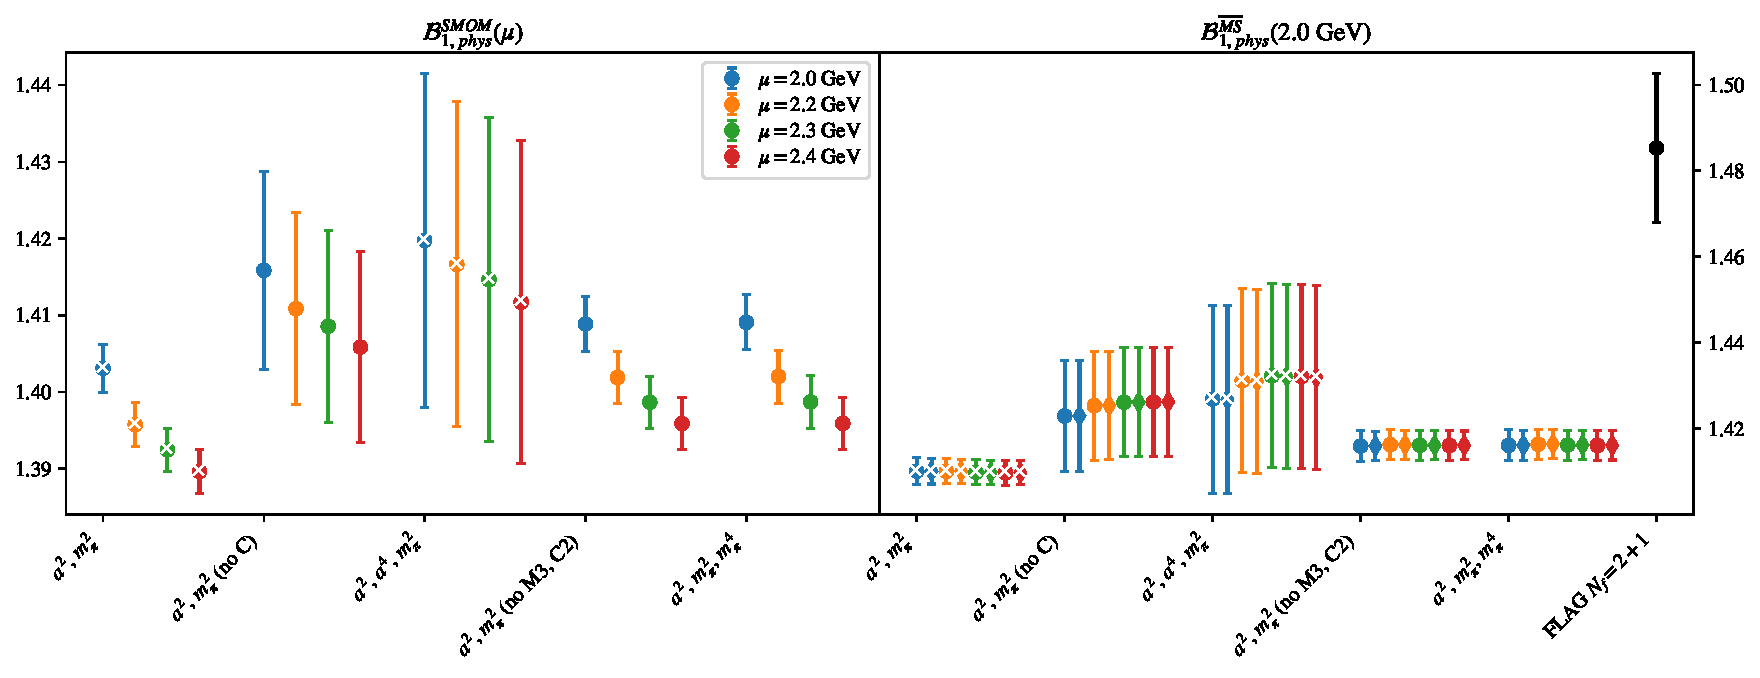
\includegraphics[page=1, width=1.1\textwidth]{VVpAA/SUSY/fit_summary_bag.pdf}
\caption{$\mathcal{B}_{1}$\\(left) $\mathcal{B}_{phys}$ in RI/SMOM scheme from fit variations (fits with $p$-value $<0.05$ marked with ``$\times$"). \\(right) $\mathcal{B}_{phys}$ in $\overline{MS}$ computed using $\mathcal{B}^{\overline{MS}} = R^{\overline{MS}\leftarrow SMOM}(2.0)\sigma_{npt}(2.0,\mu) \mathcal{B}^{SMOM}(\mu)$.}
\end{figure}
\clearpage
\begin{figure}
\centering
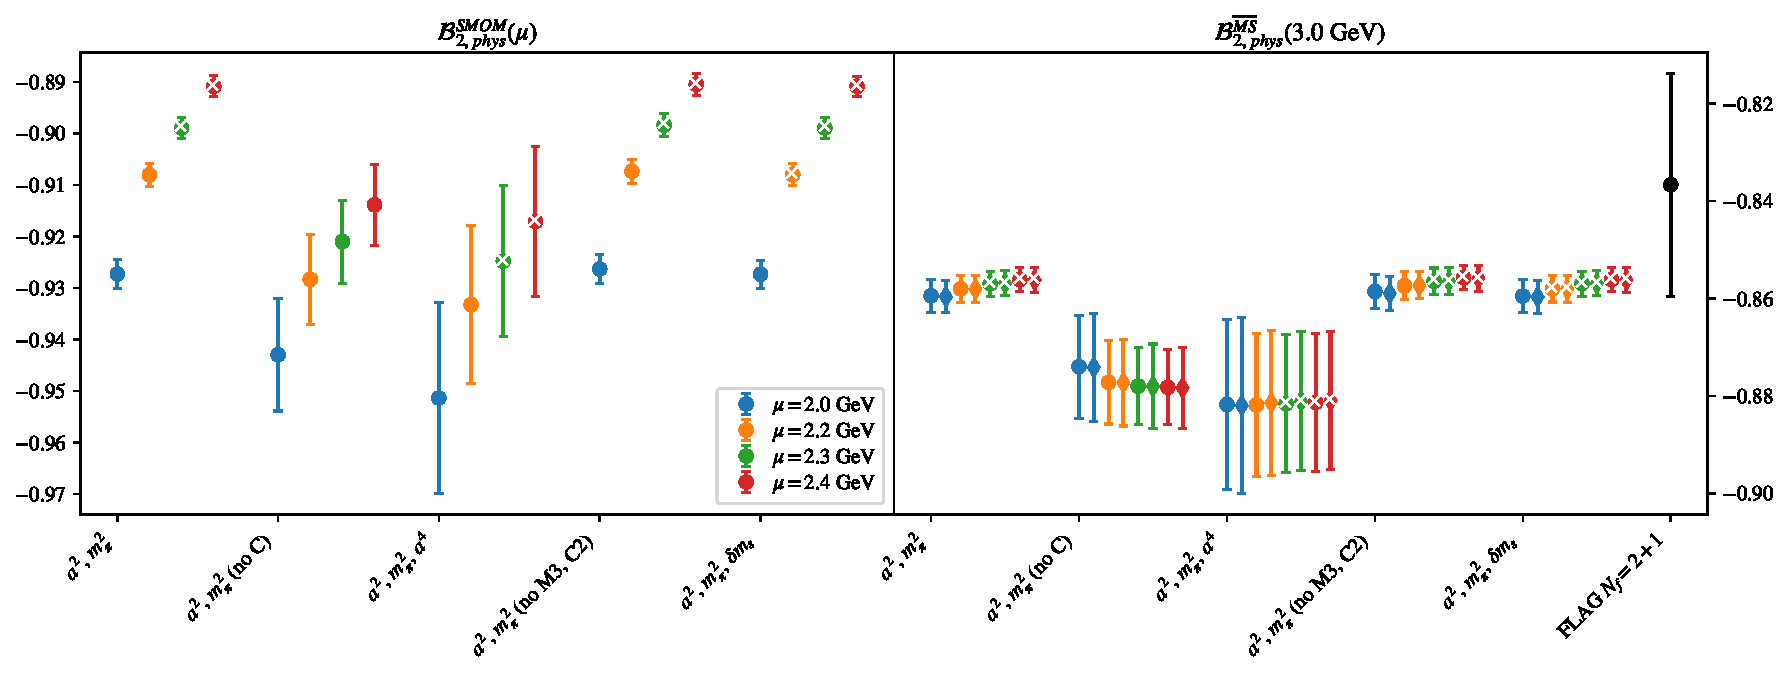
\includegraphics[page=1, width=1.1\textwidth]{VVmAA/SUSY/fit_summary_bag.pdf}
\caption{$\mathcal{B}_{2}$\\(left) $\mathcal{B}_{phys}$ in RI/SMOM scheme from fit variations (fits with $p$-value $<0.05$ marked with ``$\times$"). \\(right) $\mathcal{B}_{phys}$ in $\overline{MS}$ computed using $\mathcal{B}^{\overline{MS}} = R^{\overline{MS}\leftarrow SMOM}(3.0)\sigma_{npt}(3.0,\mu) \mathcal{B}^{SMOM}(\mu)$.}
\end{figure}
\clearpage
\begin{figure}
\centering
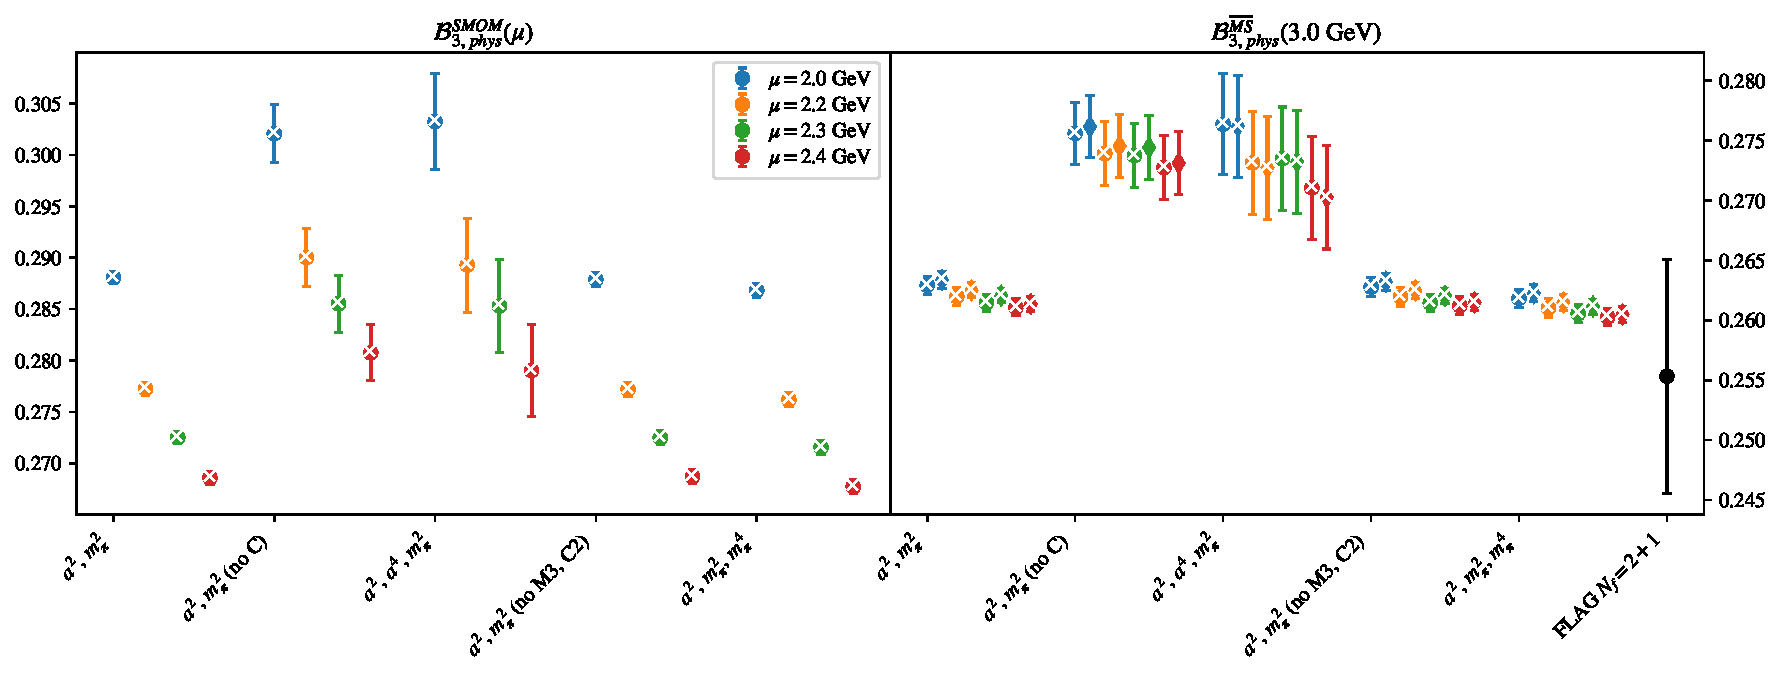
\includegraphics[page=1, width=1.1\textwidth]{SSmPP/SUSY/fit_summary_bag.pdf}
\caption{$\mathcal{B}_{3}$\\(left) $\mathcal{B}_{phys}$ in RI/SMOM scheme from fit variations (fits with $p$-value $<0.05$ marked with ``$\times$"). \\(right) $\mathcal{B}_{phys}$ in $\overline{MS}$ computed using $\mathcal{B}^{\overline{MS}} = R^{\overline{MS}\leftarrow SMOM}(3.0)\sigma_{npt}(3.0,\mu) \mathcal{B}^{SMOM}(\mu)$.}
\end{figure}
\clearpage
\begin{figure}
\centering
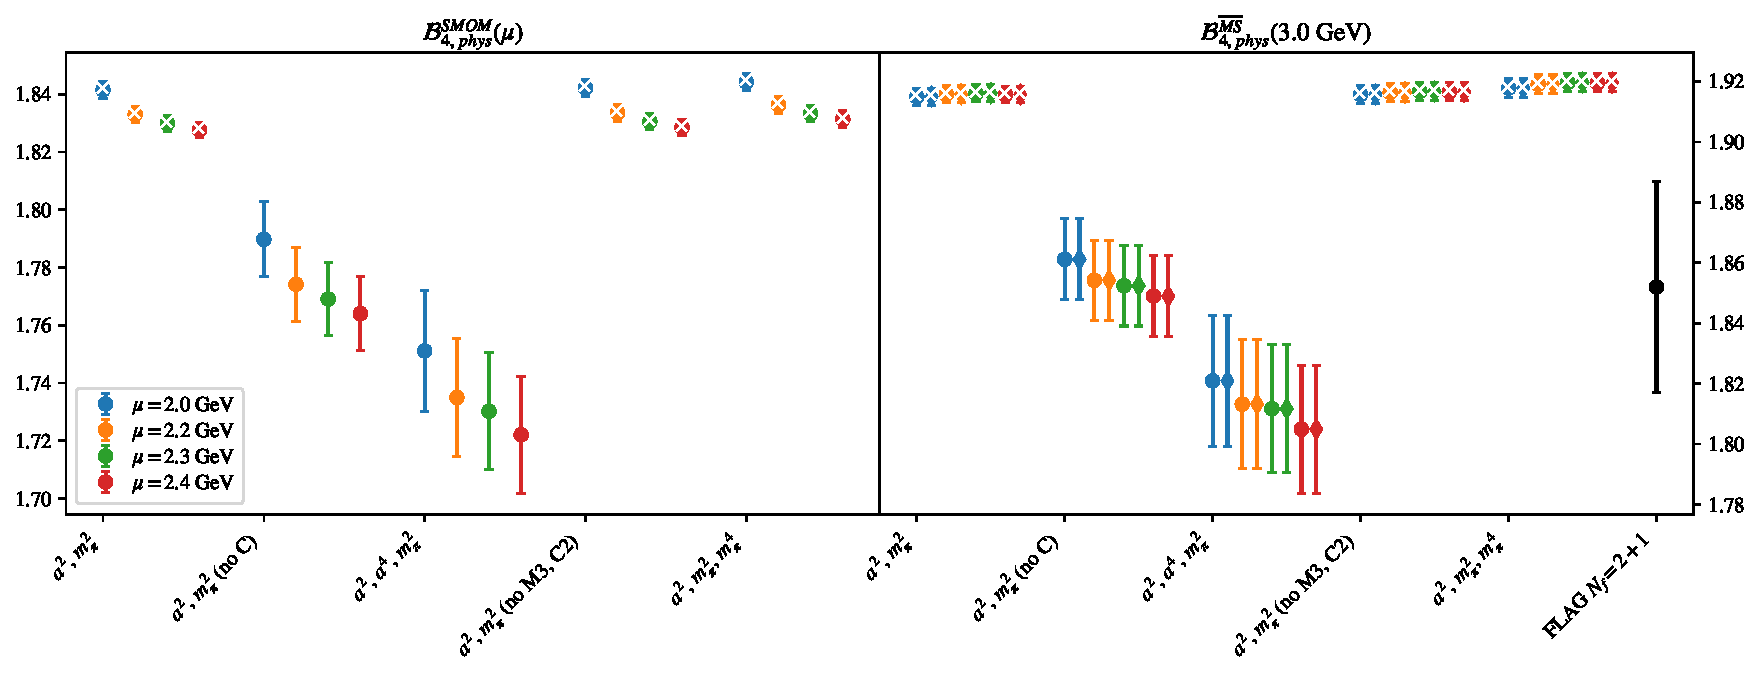
\includegraphics[page=1, width=1.1\textwidth]{SSpPP/SUSY/fit_summary_bag.pdf}
\caption{$\mathcal{B}_{4}$\\(left) $\mathcal{B}_{phys}$ in RI/SMOM scheme from fit variations (fits with $p$-value $<0.05$ marked with ``$\times$"). \\(right) $\mathcal{B}_{phys}$ in $\overline{MS}$ computed using $\mathcal{B}^{\overline{MS}} = R^{\overline{MS}\leftarrow SMOM}(3.0)\sigma_{npt}(3.0,\mu) \mathcal{B}^{SMOM}(\mu)$.}
\end{figure}
\clearpage
\begin{figure}
\centering
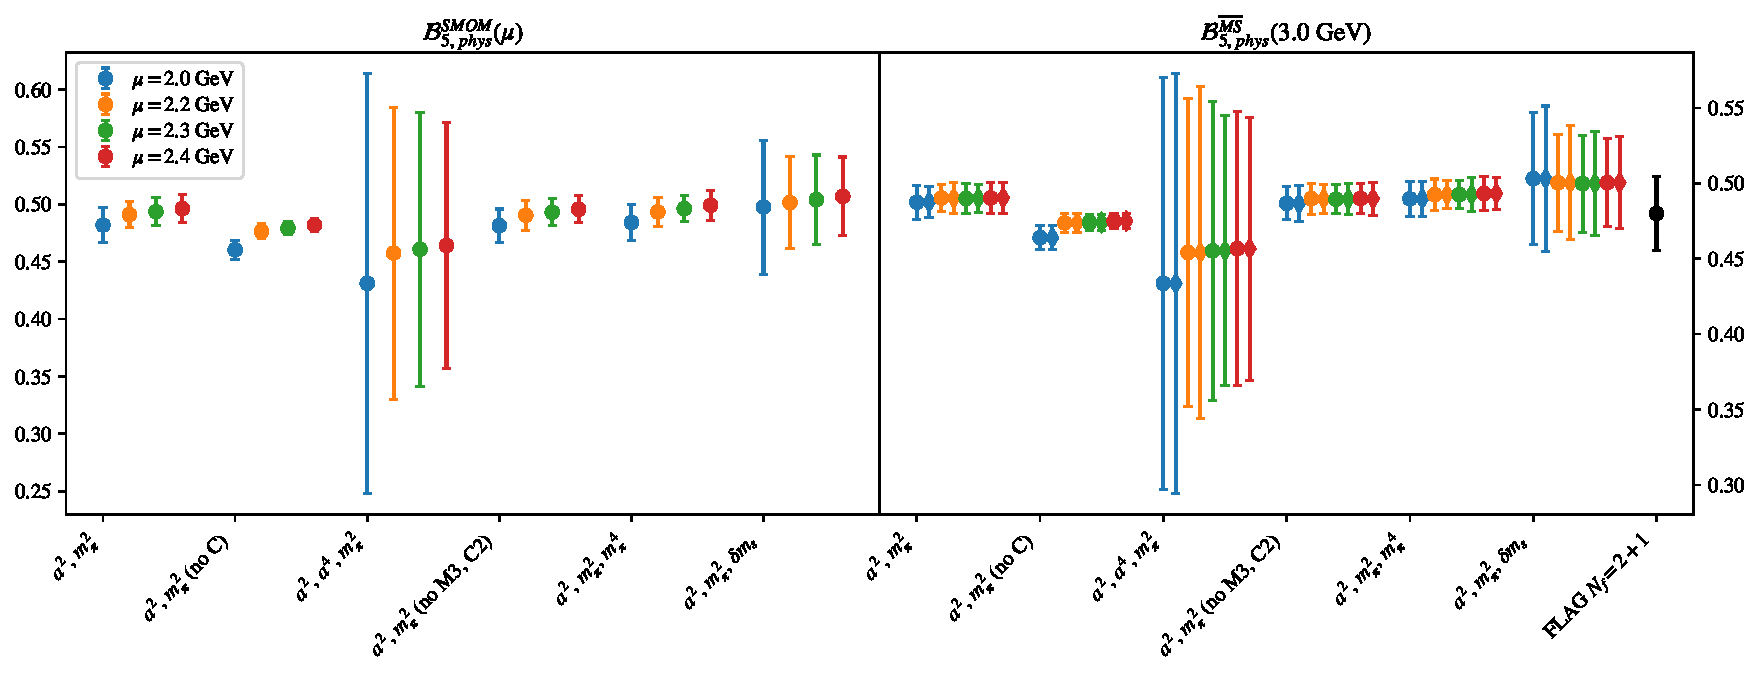
\includegraphics[page=1, width=1.1\textwidth]{TT/SUSY/fit_summary_bag.pdf}
\caption{$\mathcal{B}_{5}$\\(left) $\mathcal{B}_{phys}$ in RI/SMOM scheme from fit variations (fits with $p$-value $<0.05$ marked with ``$\times$"). \\(right) $\mathcal{B}_{phys}$ in $\overline{MS}$ computed using $\mathcal{B}^{\overline{MS}} = R^{\overline{MS}\leftarrow SMOM}(3.0)\sigma_{npt}(3.0,\mu) \mathcal{B}^{SMOM}(\mu)$.}
\end{figure}
\clearpage
\section{$\mathcal{B}_1$}
\begin{table}[h!]
\begin{center}
\begin{tabular}{|c|c|c|c|c|c|}
\hline
$\mu$ (GeV) & $a^2$, $m_\pi^2$& $a^2$, $m_\pi^2$ (no C)& $a^2$, $a^4$, $m_\pi^2$& $a^2$, $m_\pi^2$ (no M3, C2)& $a^2$, $m_\pi^2$, $m_\pi^4$\\
\hline
2.0& \hyperlink{VVpAA/SUSY/a2m2_20.pdf.1}{\textbf{1.4030(29)}: 2.3 (0.042)} & \hyperlink{VVpAA/SUSY/a2m2noC_20.pdf.1}{\textbf{1.415(12)}: 1.025 (0.359)} & \hyperlink{VVpAA/SUSY/a2a4m2_20.pdf.1}{\textbf{1.419(21)}: 2.737 (0.027)} & \hyperlink{VVpAA/SUSY/a2m2mcut_20.pdf.1}{\textbf{1.4088(34)}: 0.233 (0.873)} & \hyperlink{VVpAA/SUSY/a2m2m4_20.pdf.1}{\textbf{1.4090(34)}: 0.779 (0.539)}\\
2.2& \hyperlink{VVpAA/SUSY/a2m2_22.pdf.1}{\textbf{1.3957(27)}: 2.577 (0.024)} & \hyperlink{VVpAA/SUSY/a2m2noC_22.pdf.1}{\textbf{1.410(12)}: 1.152 (0.316)} & \hyperlink{VVpAA/SUSY/a2a4m2_22.pdf.1}{\textbf{1.416(21)}: 2.986 (0.018)} & \hyperlink{VVpAA/SUSY/a2m2mcut_22.pdf.1}{\textbf{1.4018(33)}: 0.348 (0.791)} & \hyperlink{VVpAA/SUSY/a2m2m4_22.pdf.1}{\textbf{1.4019(33)}: 1.025 (0.393)}\\
2.3& \hyperlink{VVpAA/SUSY/a2m2_23.pdf.1}{\textbf{1.3924(27)}: 2.685 (0.02)} & \hyperlink{VVpAA/SUSY/a2m2noC_23.pdf.1}{\textbf{1.408(12)}: 1.184 (0.306)} & \hyperlink{VVpAA/SUSY/a2a4m2_23.pdf.1}{\textbf{1.414(21)}: 3.086 (0.015)} & \hyperlink{VVpAA/SUSY/a2m2mcut_23.pdf.1}{\textbf{1.3986(33)}: 0.4 (0.753)} & \hyperlink{VVpAA/SUSY/a2m2m4_23.pdf.1}{\textbf{1.3987(33)}: 1.129 (0.341)}\\
2.4& \hyperlink{VVpAA/SUSY/a2m2_24.pdf.1}{\textbf{1.3896(27)}: 2.716 (0.019)} & \hyperlink{VVpAA/SUSY/a2m2noC_24.pdf.1}{\textbf{1.405(12)}: 1.192 (0.304)} & \hyperlink{VVpAA/SUSY/a2a4m2_24.pdf.1}{\textbf{1.411(21)}: 3.126 (0.014)} & \hyperlink{VVpAA/SUSY/a2m2mcut_24.pdf.1}{\textbf{1.3958(32)}: 0.401 (0.752)} & \hyperlink{VVpAA/SUSY/a2m2m4_24.pdf.1}{\textbf{1.3958(33)}: 1.147 (0.332)}\\
\hline
\end{tabular}
\caption{Physical point value from chiral and continuum extrapolation at renormalisation scale $\mu$. Entries are \textbf{value(error)}: $\chi^2/\text{DOF}$ ($p$-value).}
\end{center}
\end{table}
\begin{table}[h!]
\begin{center}
\begin{tabular}{|c c|c|c|c|c|c|}
\hline
$\mu$ (GeV) &  & $a^2$, $m_\pi^2$& $a^2$, $m_\pi^2$ (no C)& $a^2$, $a^4$, $m_\pi^2$& $a^2$, $m_\pi^2$ (no M3, C2)& $a^2$, $m_\pi^2$, $m_\pi^4$\\
\hline
\multirow{2}{0.5in}{2.0} & $\alpha$ & 0.0954(73)& 0.048(53)& -0.013& 0.0816(84)& 0.0816(83)\\
 & $\beta$ & 0.00270(14)& 0.00225(27)& 0.00272(15)& 0.00188(28)& 0.0\\
\hline
\multirow{2}{0.5in}{2.2} & $\alpha$ & 0.0994(70)& 0.042(52)& -0.037& 0.0846(83)& 0.0849(82)\\
 & $\beta$ & 0.00268(14)& 0.00221(27)& 0.00271(14)& 0.00184(28)& 0.0\\
\hline
\multirow{2}{0.5in}{2.3} & $\alpha$ & 0.1009(70)& 0.039(52)& -0.044& 0.0859(83)& 0.0864(82)\\
 & $\beta$ & 0.00268(14)& 0.00220(27)& 0.00271(14)& 0.00183(28)& 0.0\\
\hline
\multirow{2}{0.5in}{2.4} & $\alpha$ & 0.1016(70)& 0.039(52)& -0.043& 0.0864(83)& 0.0870(82)\\
 & $\beta$ & 0.00269(14)& 0.00219(27)& 0.00272(14)& 0.00183(28)& 0.0\\
\hline
\end{tabular}
\caption{Fit values of coefficients in $Q = Q_{phys} + \mathbf{\alpha} a^2 + \mathbf{\beta}\left(\frac{m_\pi^2}{f_\pi^2}-\frac{m_{\pi,PDG}^2}{f_\pi^2}\right) + \ldots$.}
\end{center}
\end{table}
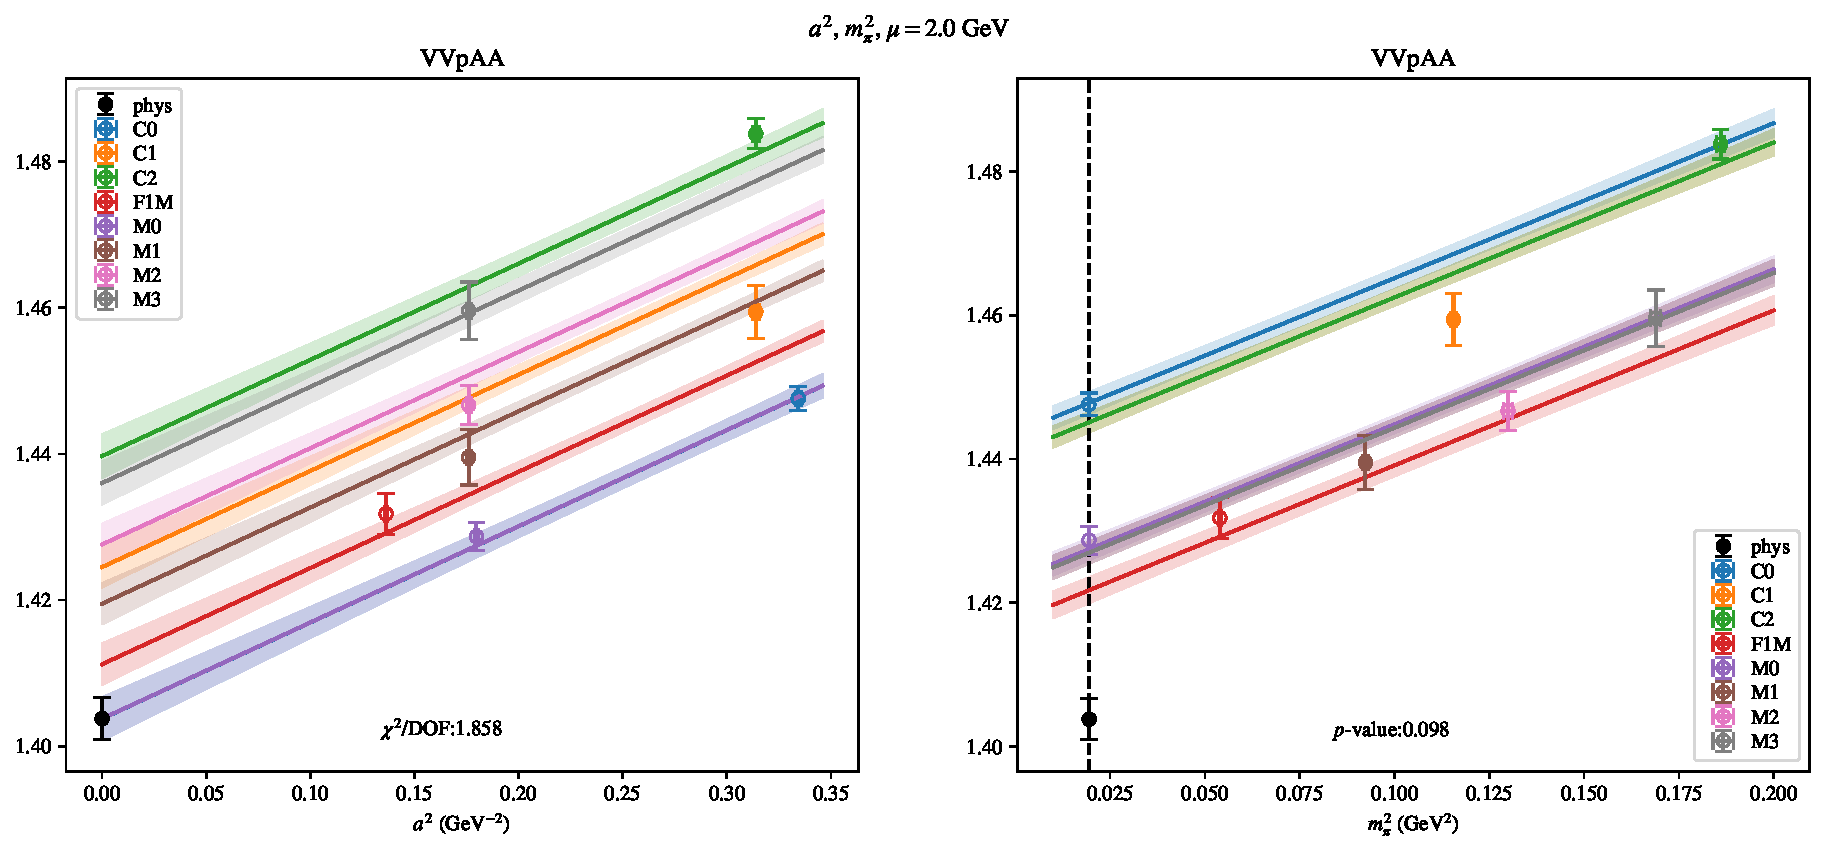
\includepdf[link, pages=-]{VVpAA/SUSY/a2m2_20.pdf}
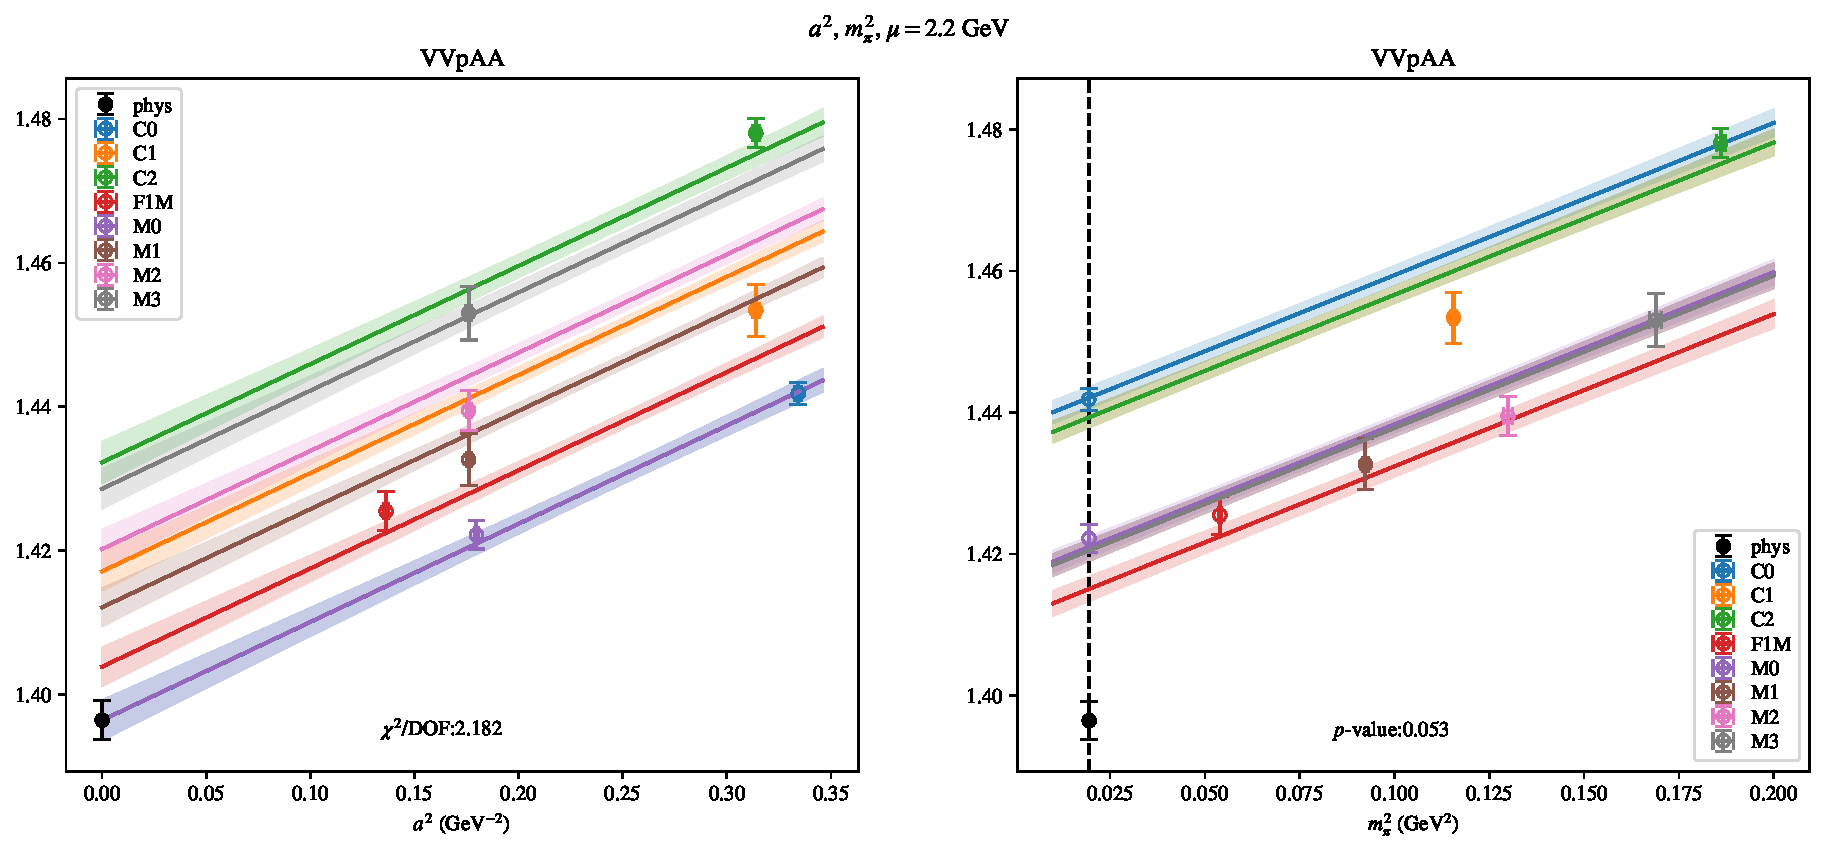
\includepdf[link, pages=-]{VVpAA/SUSY/a2m2_22.pdf}
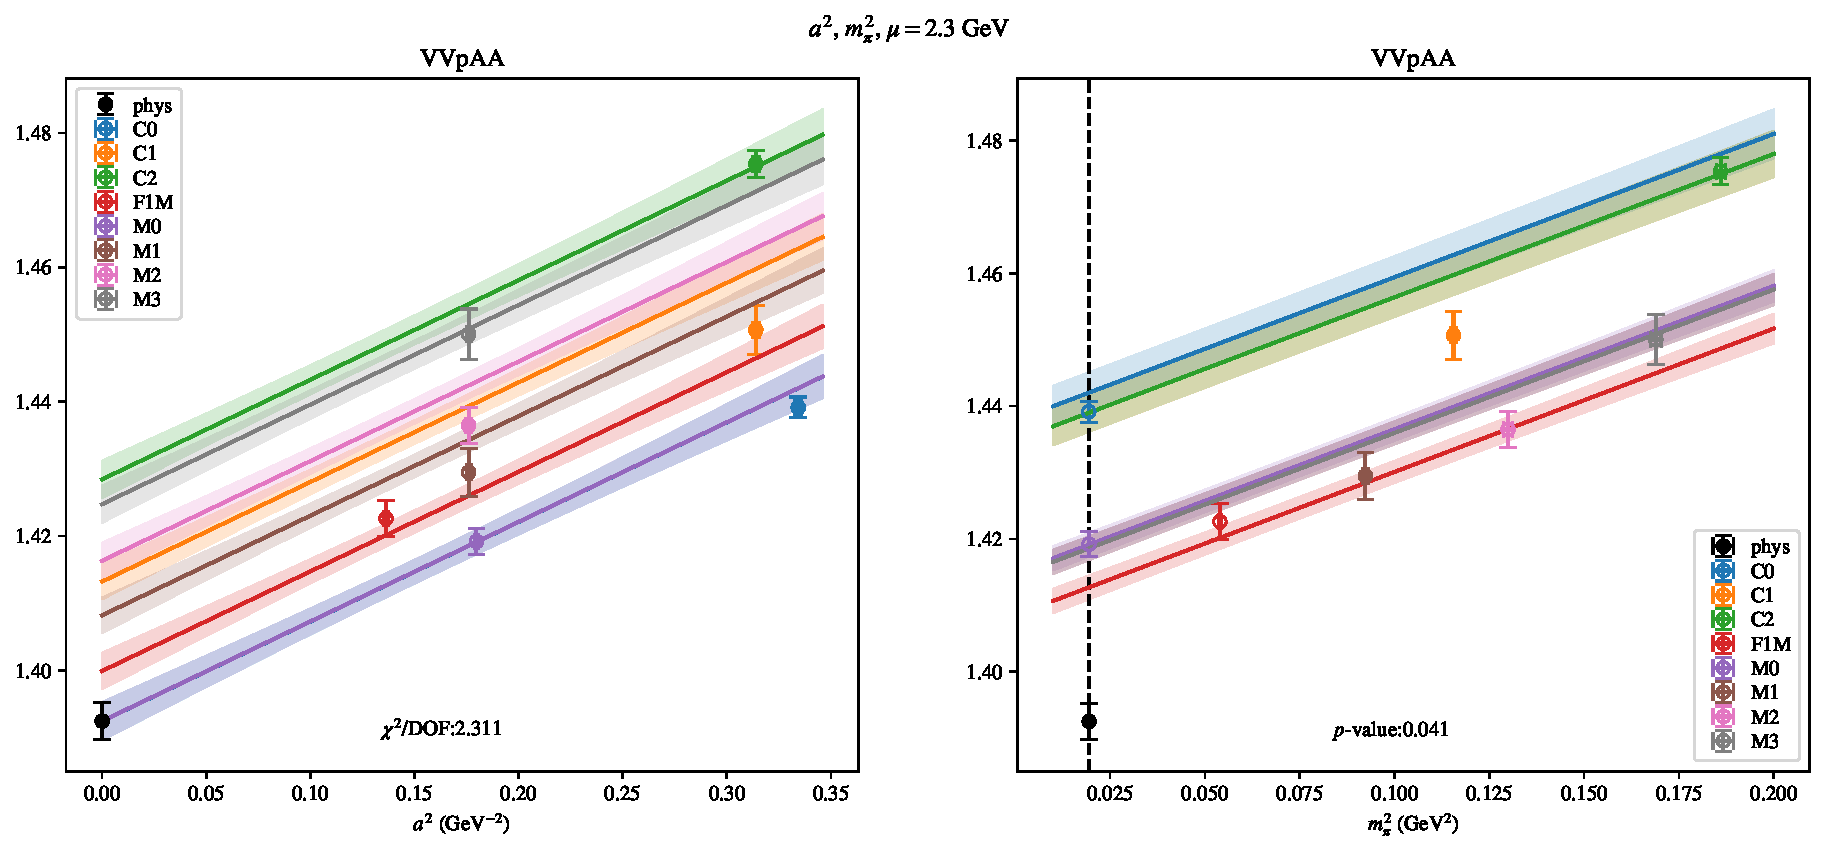
\includepdf[link, pages=-]{VVpAA/SUSY/a2m2_23.pdf}
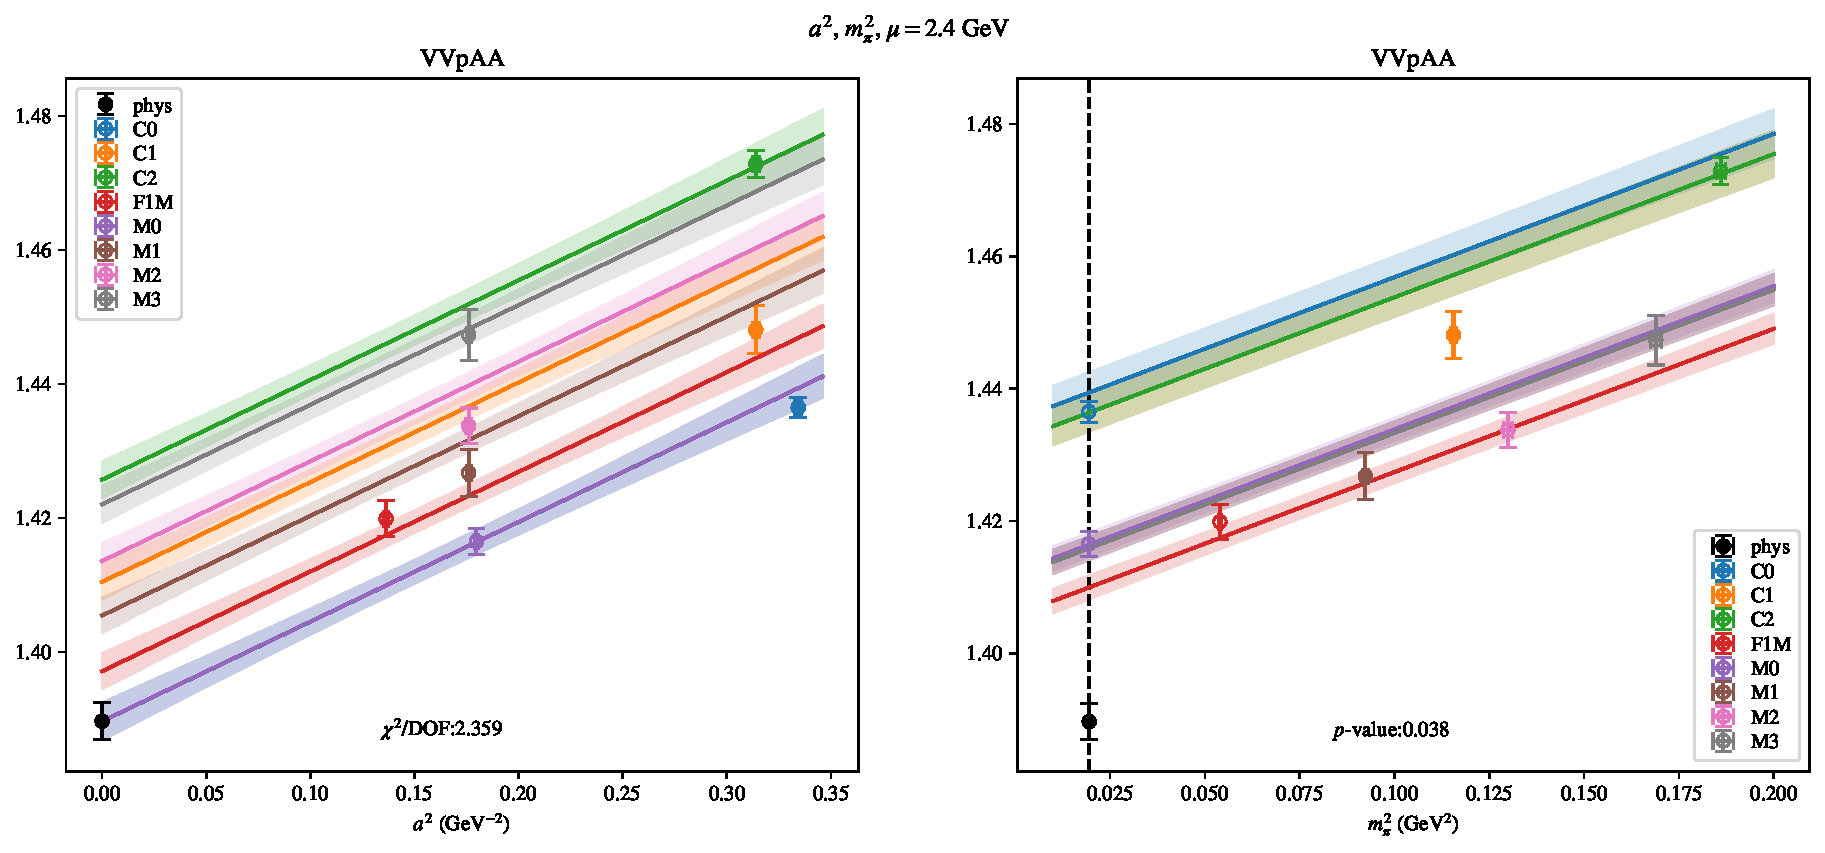
\includepdf[link, pages=-]{VVpAA/SUSY/a2m2_24.pdf}
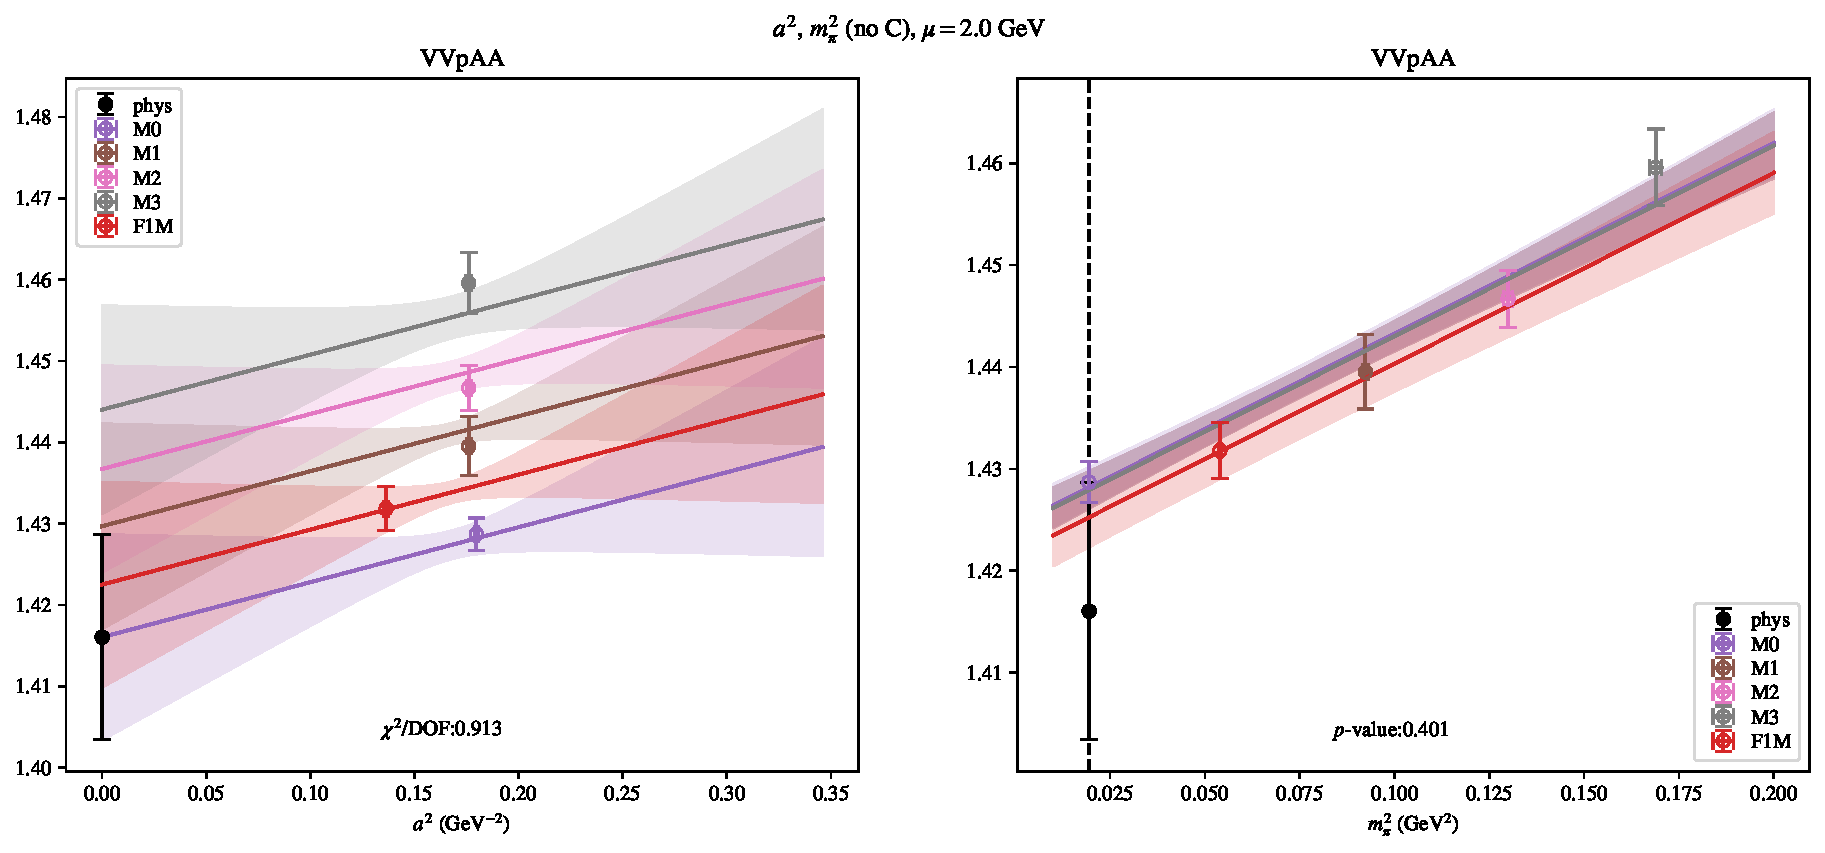
\includepdf[link, pages=-]{VVpAA/SUSY/a2m2noC_20.pdf}
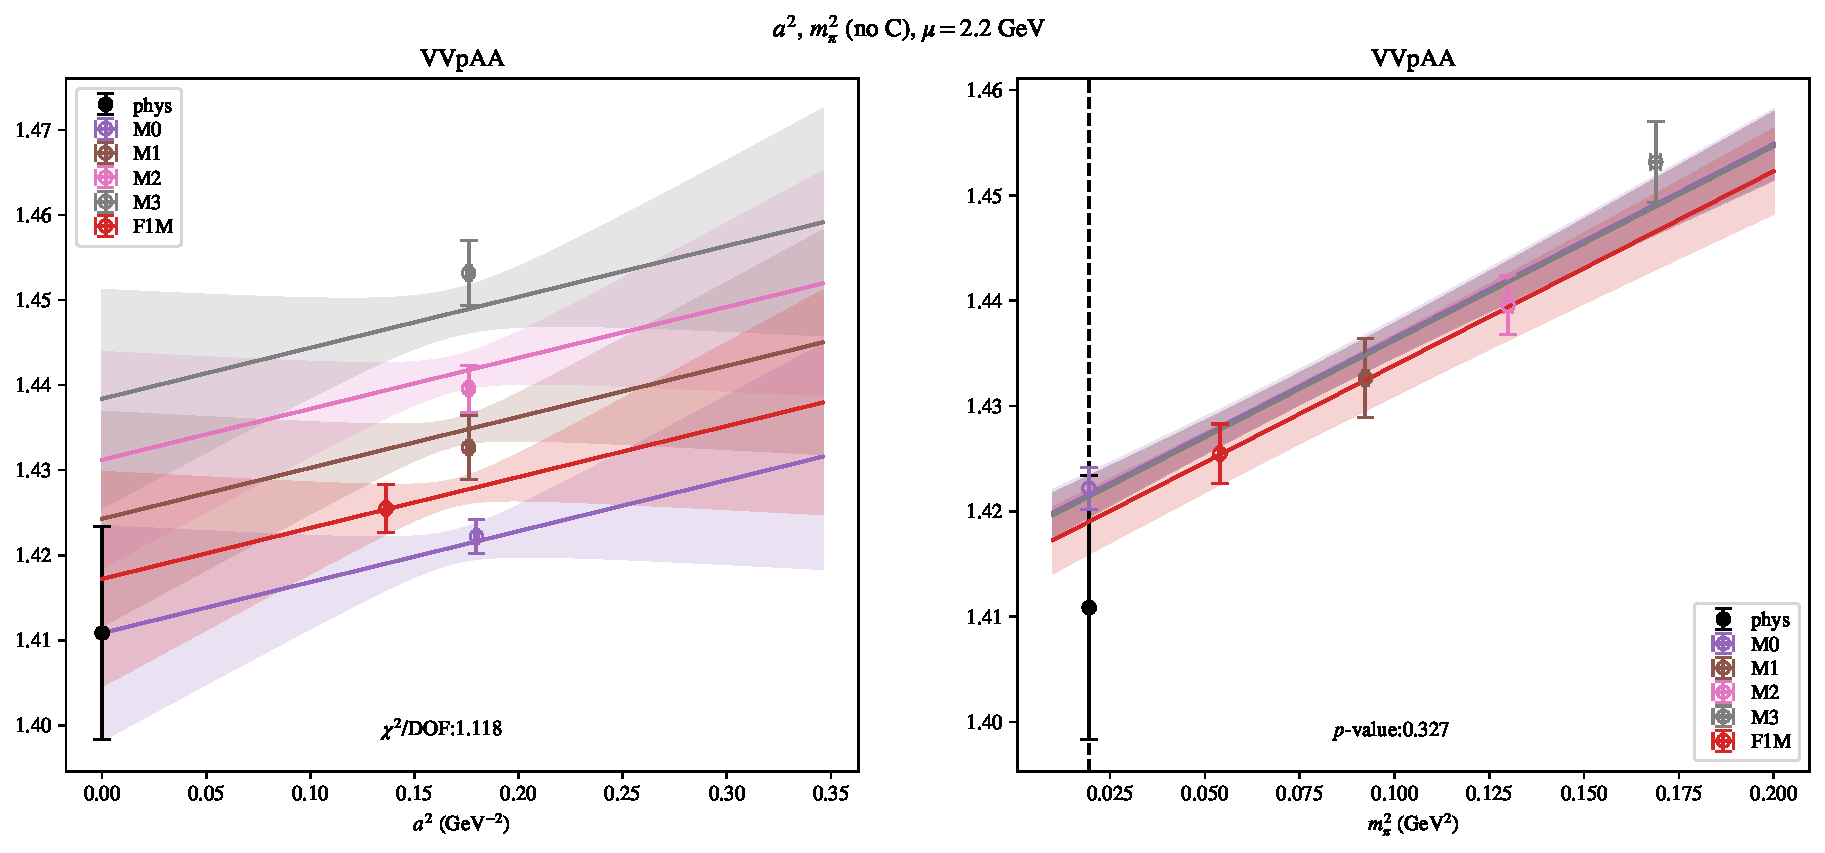
\includepdf[link, pages=-]{VVpAA/SUSY/a2m2noC_22.pdf}
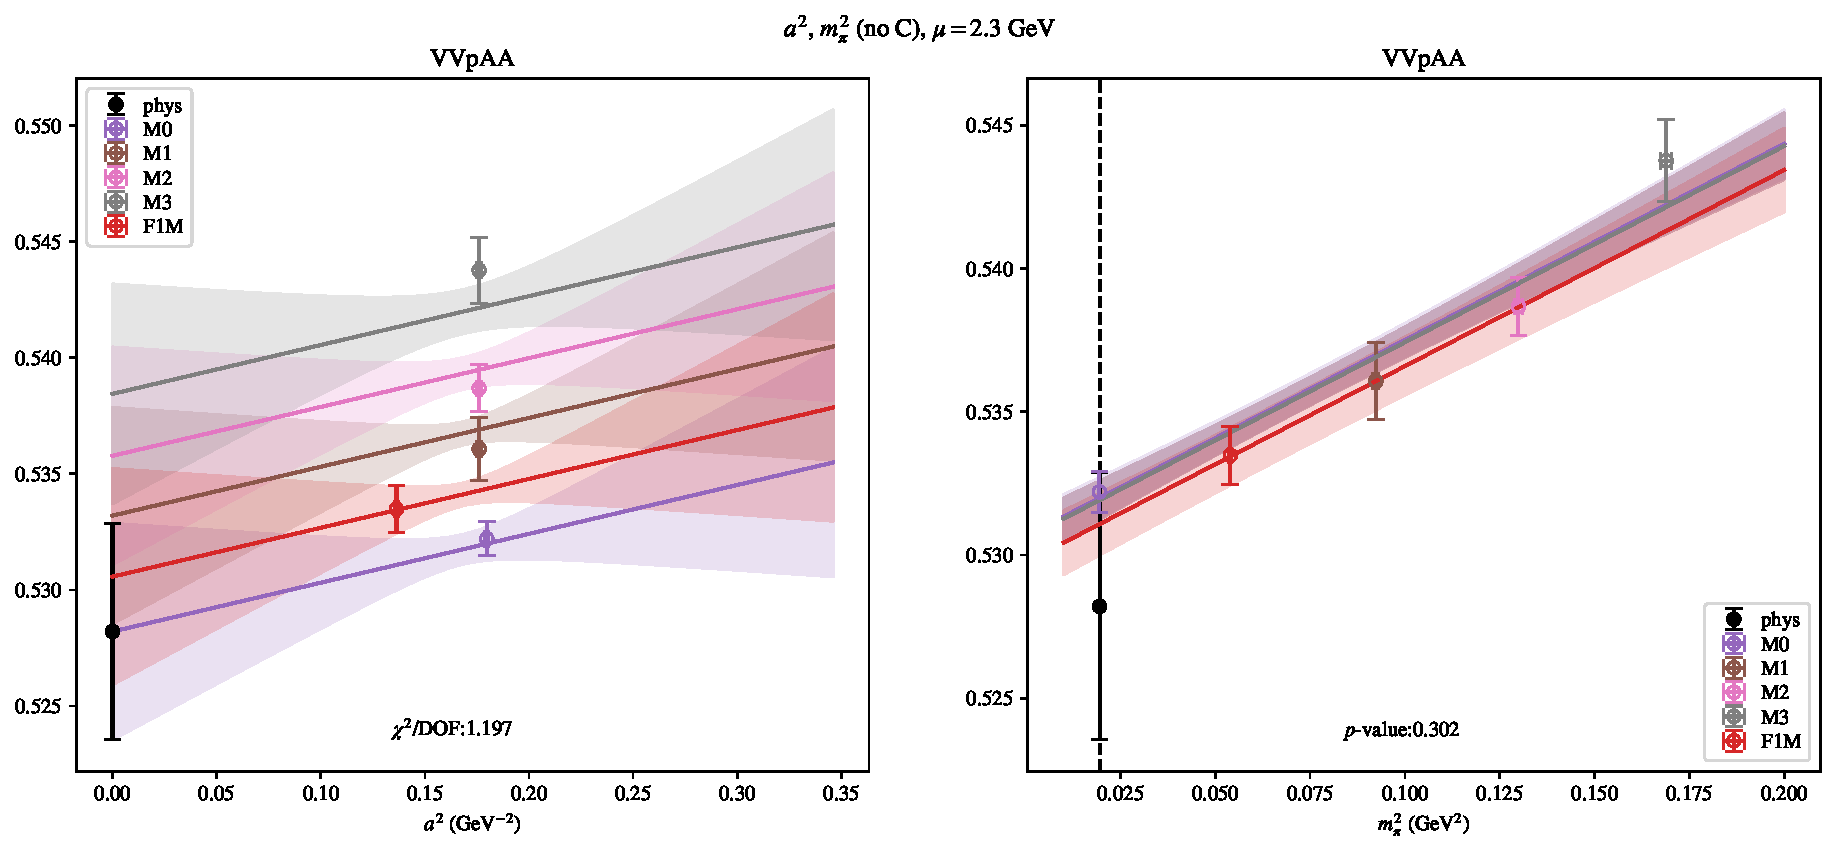
\includepdf[link, pages=-]{VVpAA/SUSY/a2m2noC_23.pdf}
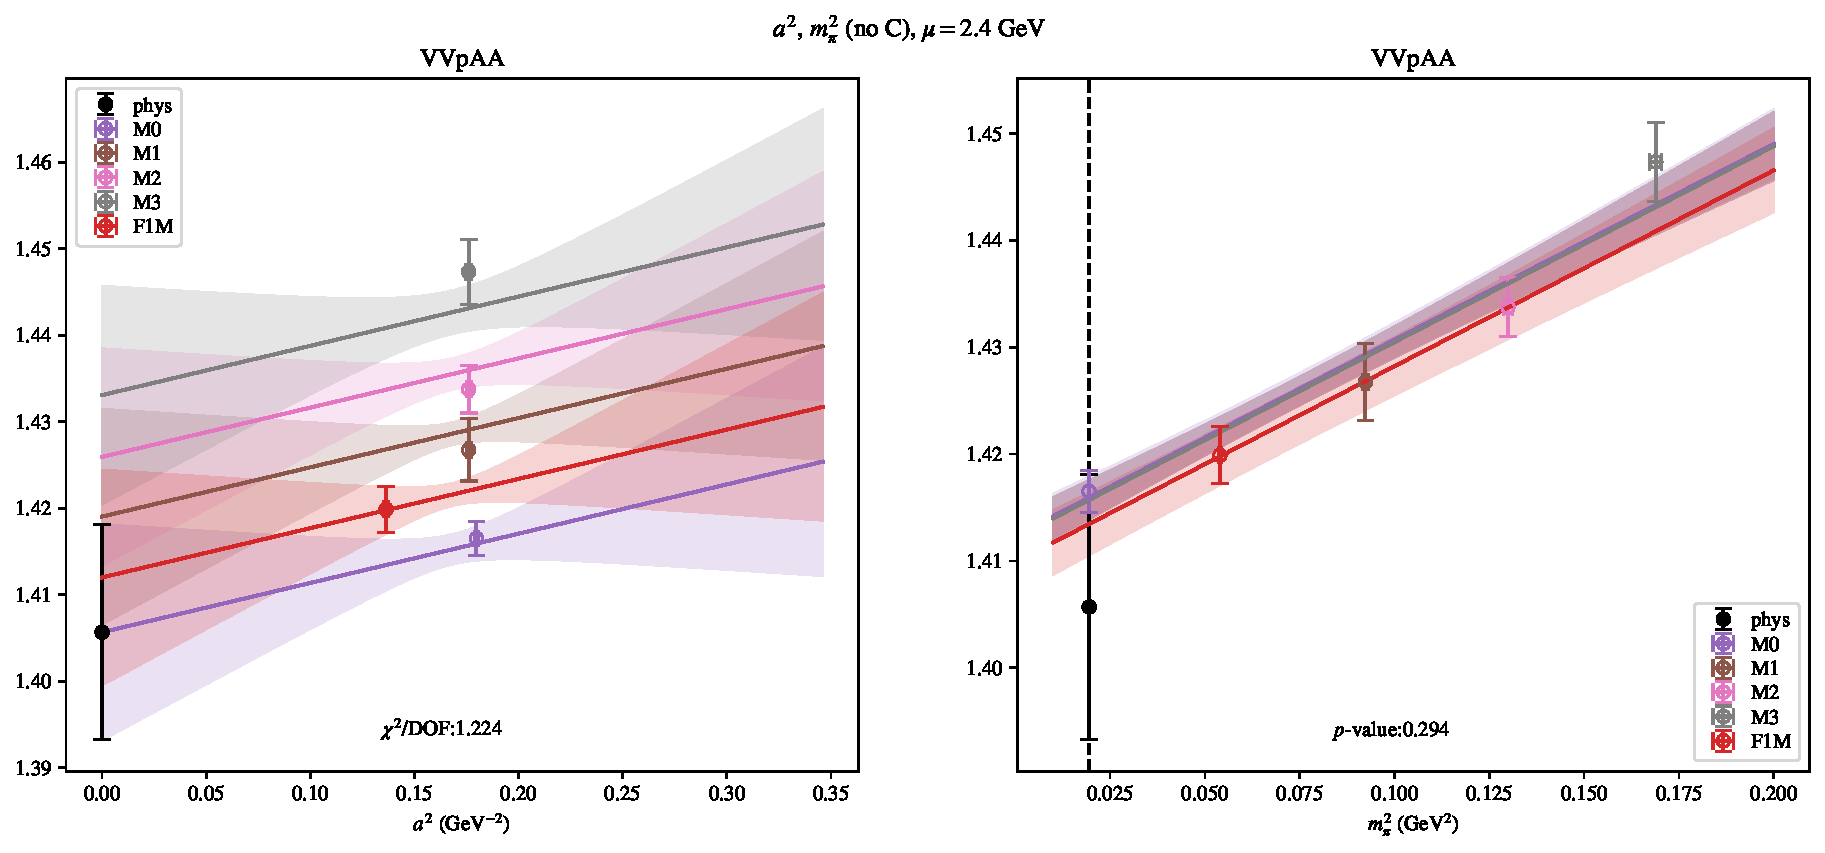
\includepdf[link, pages=-]{VVpAA/SUSY/a2m2noC_24.pdf}
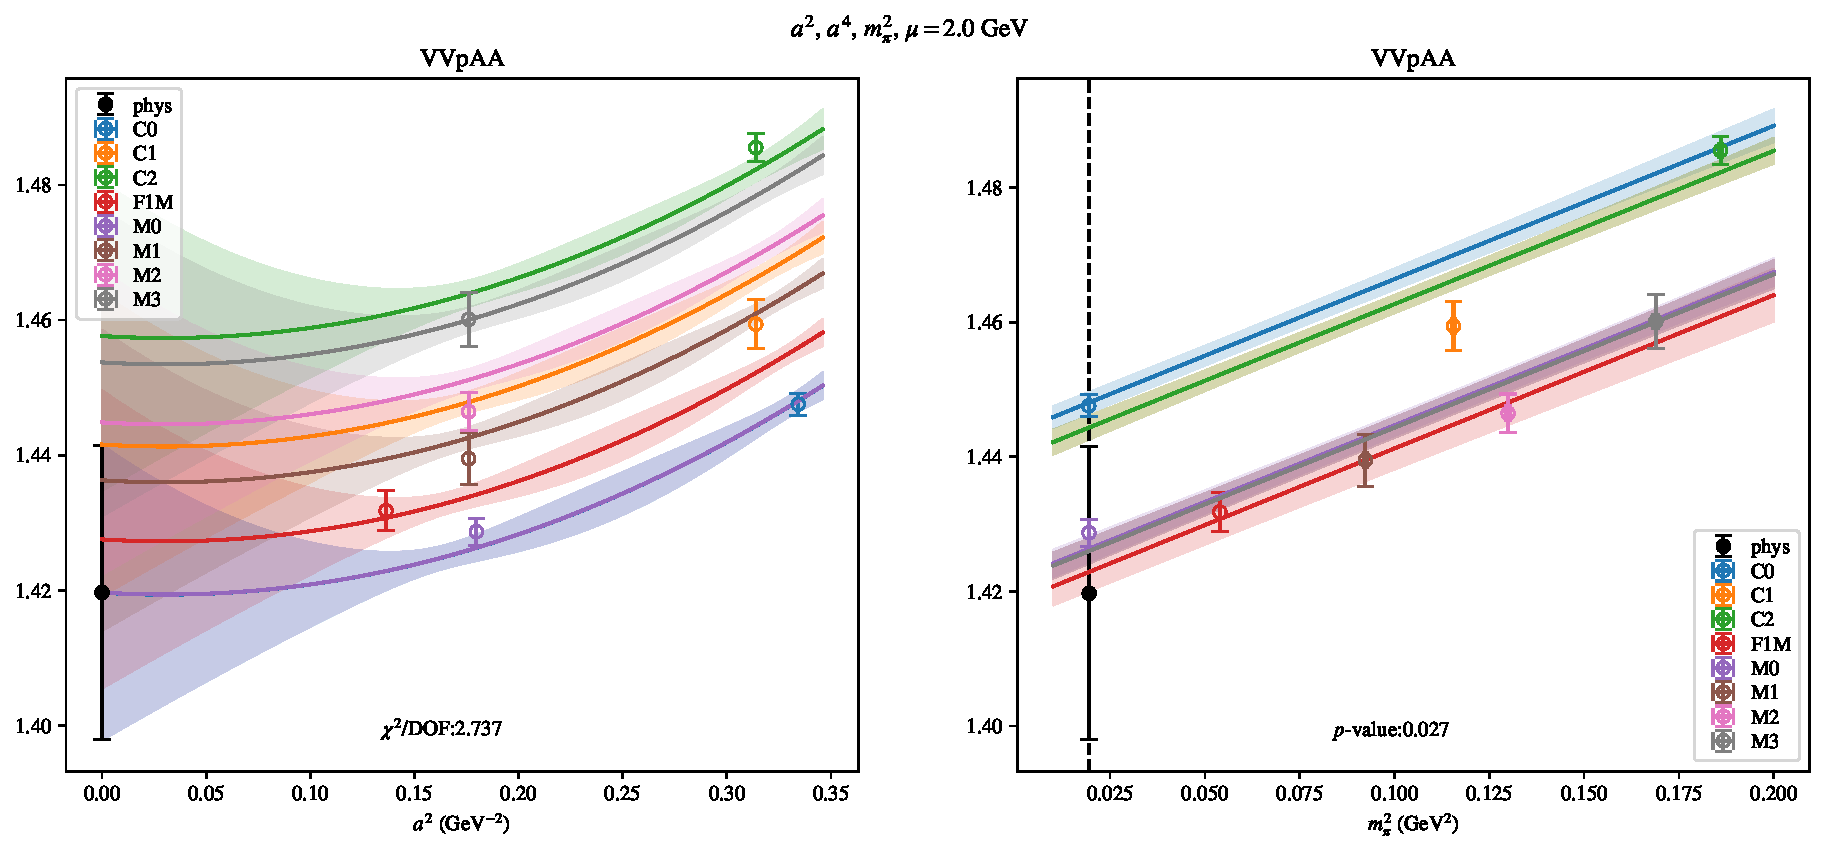
\includepdf[link, pages=-]{VVpAA/SUSY/a2a4m2_20.pdf}
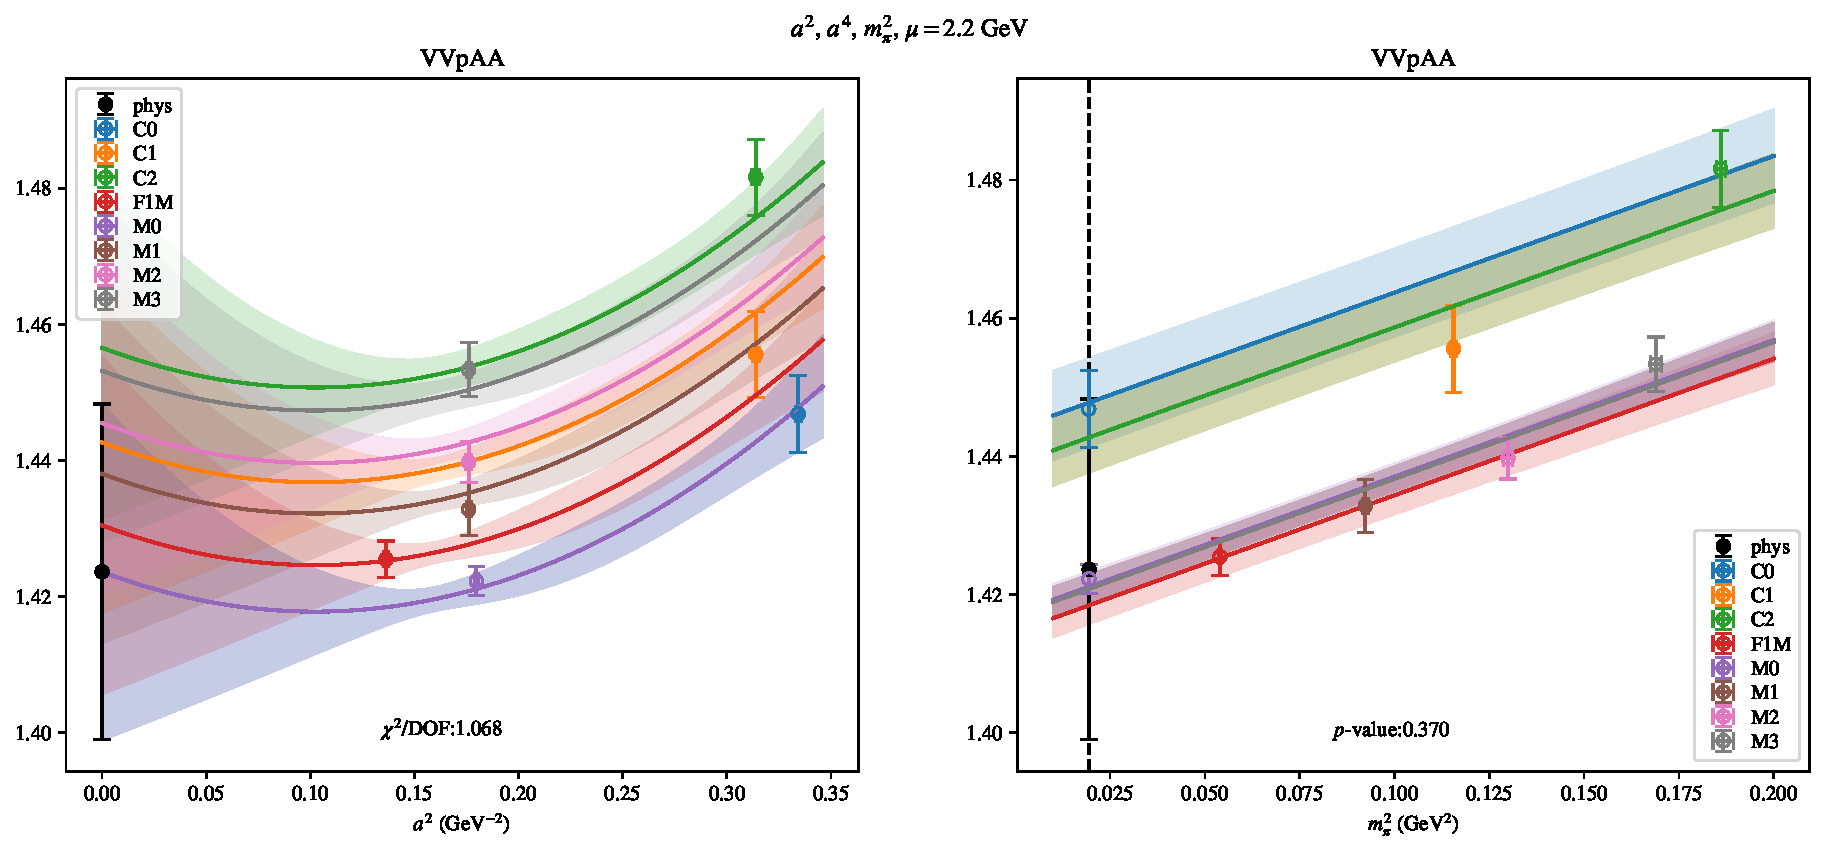
\includepdf[link, pages=-]{VVpAA/SUSY/a2a4m2_22.pdf}
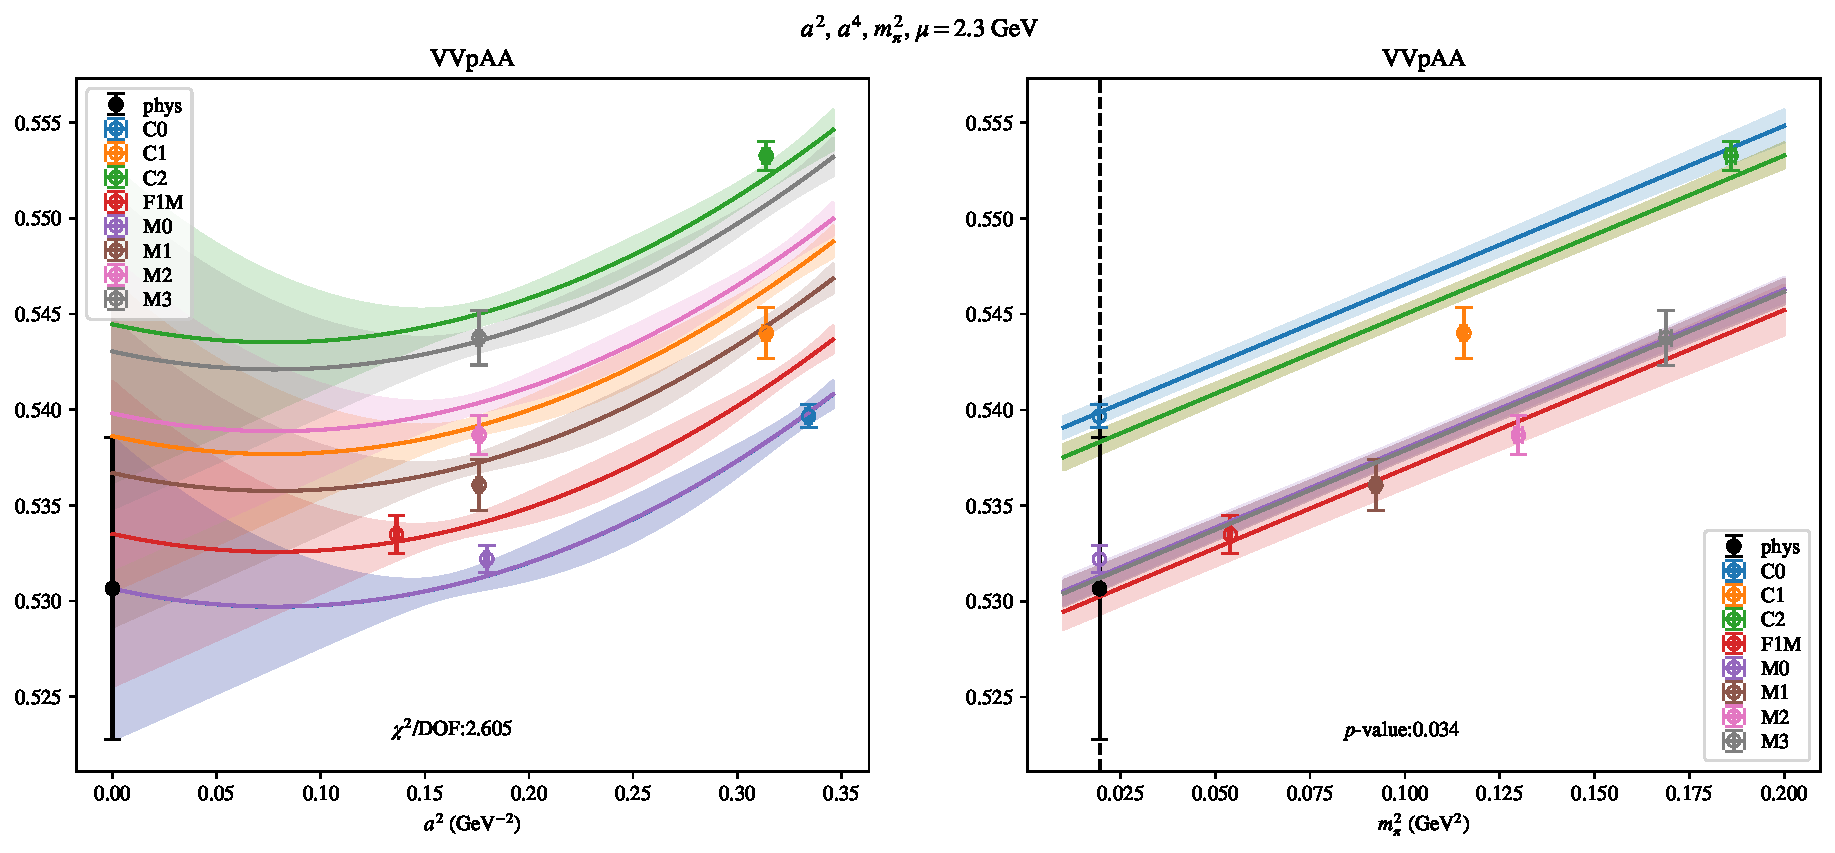
\includepdf[link, pages=-]{VVpAA/SUSY/a2a4m2_23.pdf}
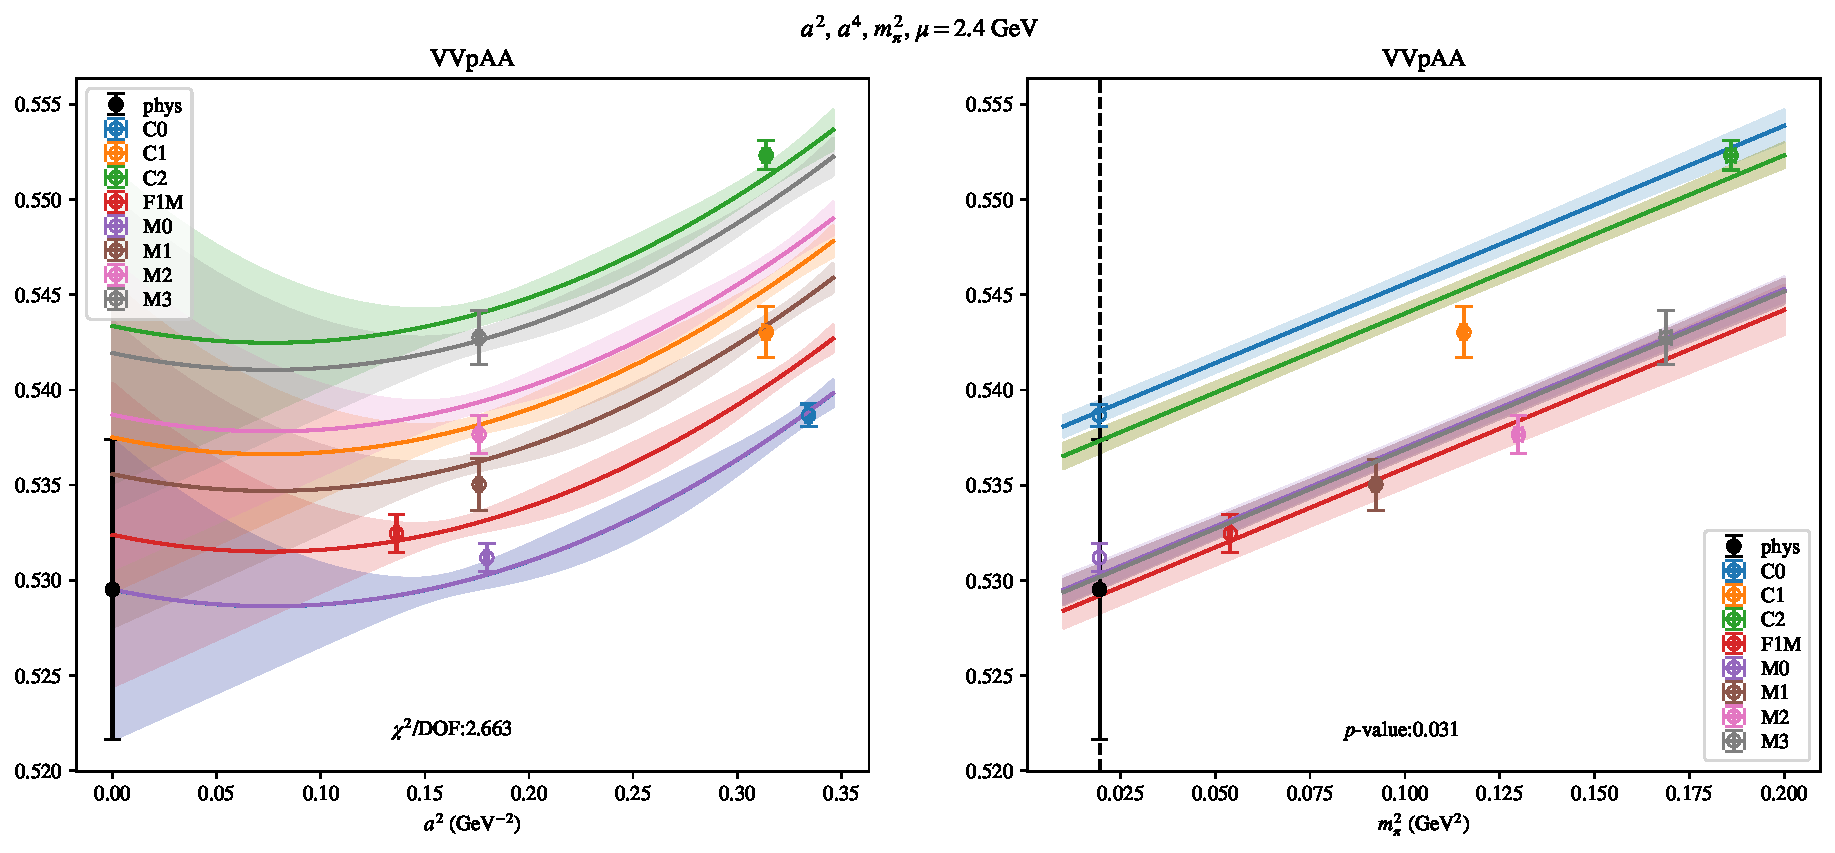
\includepdf[link, pages=-]{VVpAA/SUSY/a2a4m2_24.pdf}
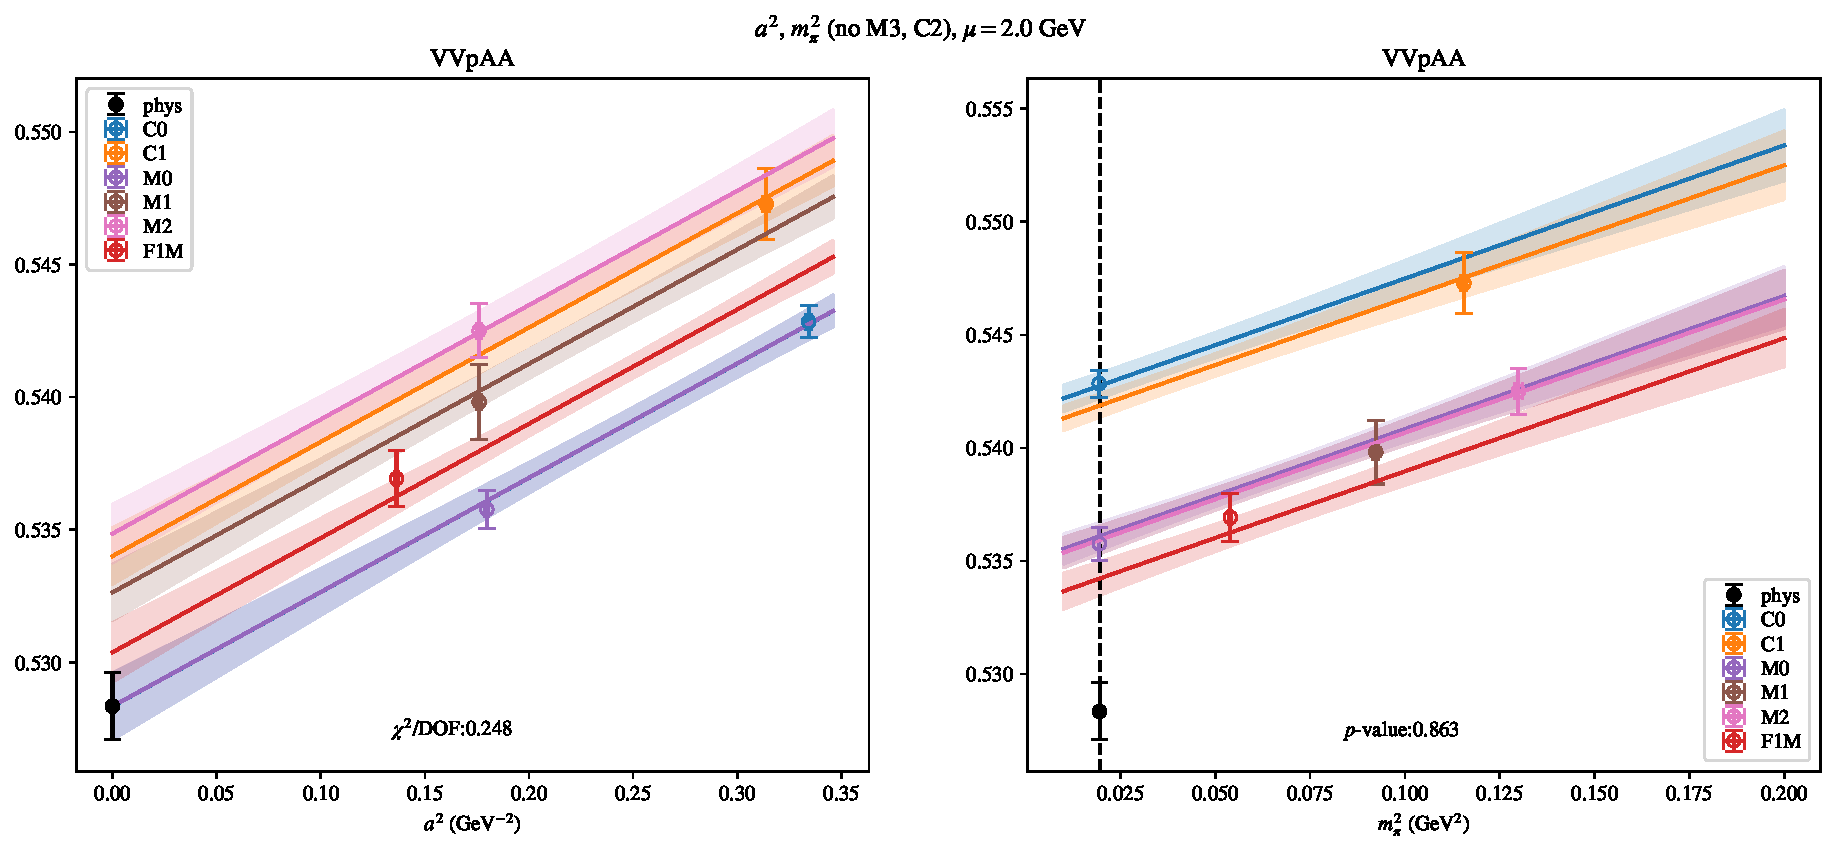
\includepdf[link, pages=-]{VVpAA/SUSY/a2m2mcut_20.pdf}
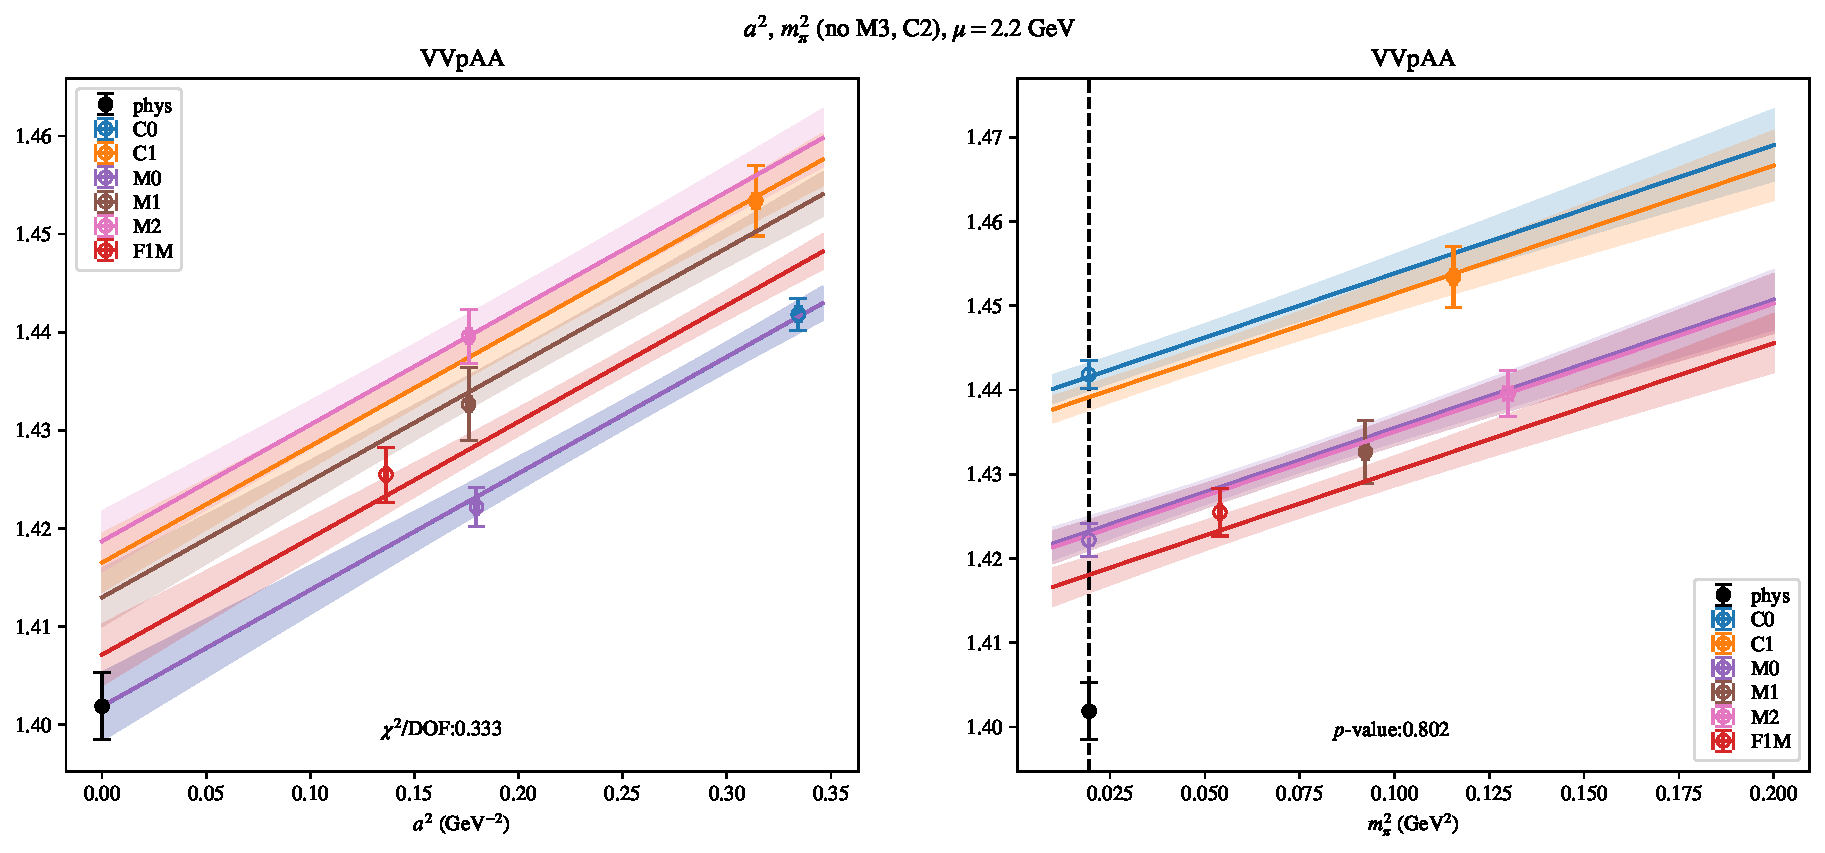
\includepdf[link, pages=-]{VVpAA/SUSY/a2m2mcut_22.pdf}
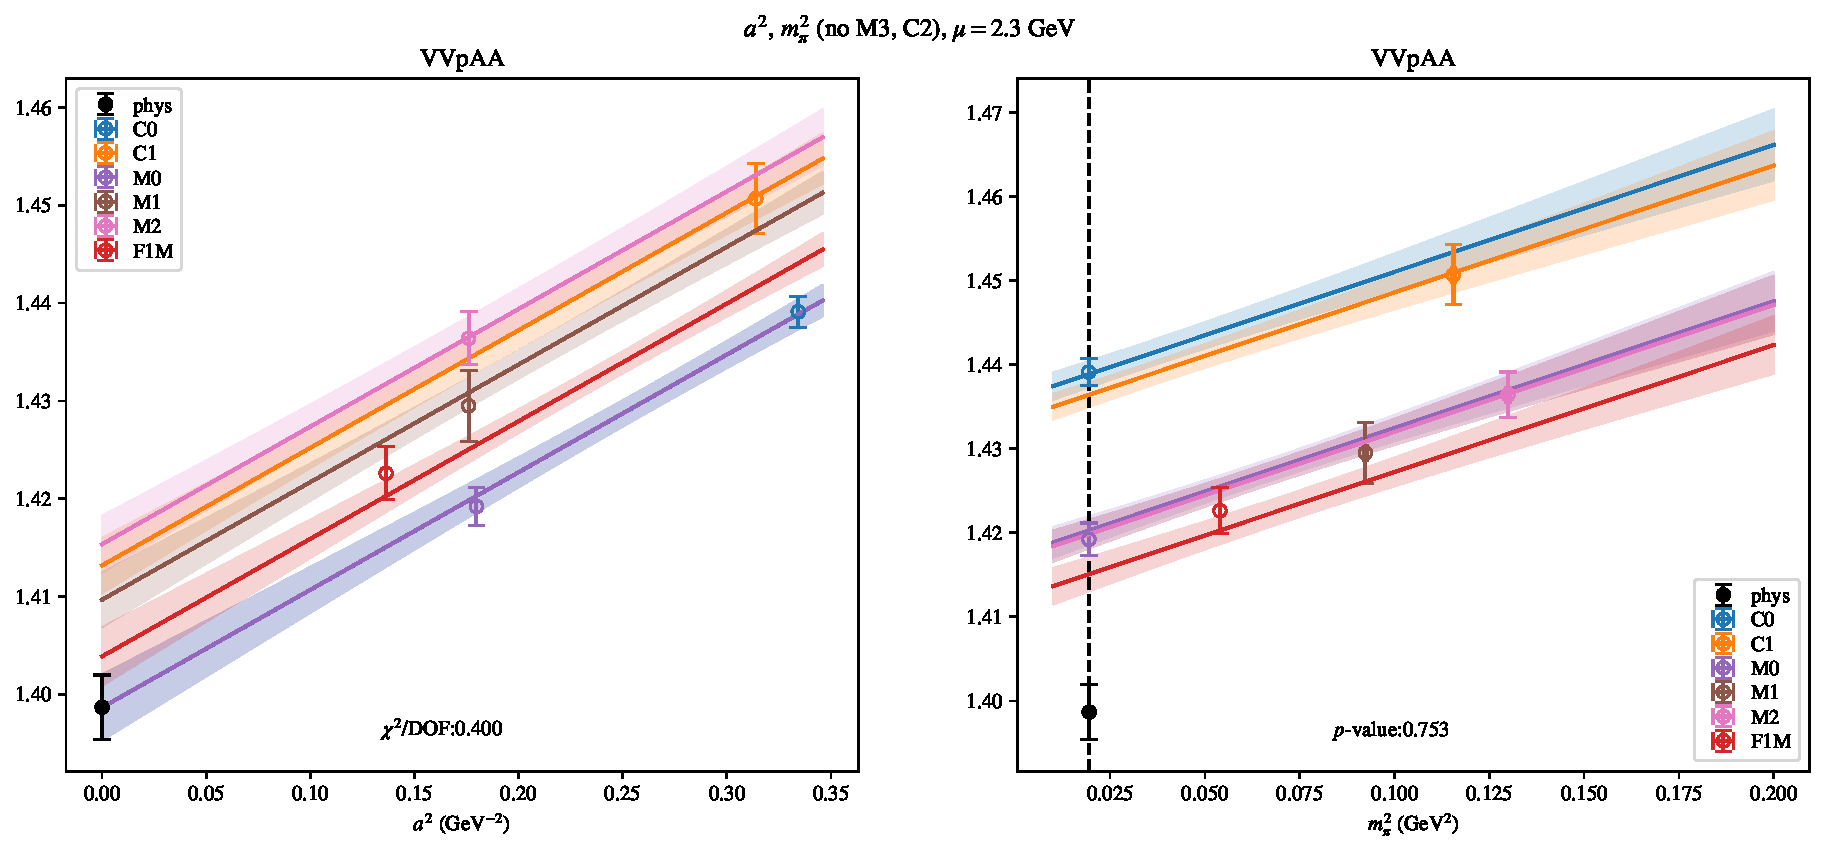
\includepdf[link, pages=-]{VVpAA/SUSY/a2m2mcut_23.pdf}
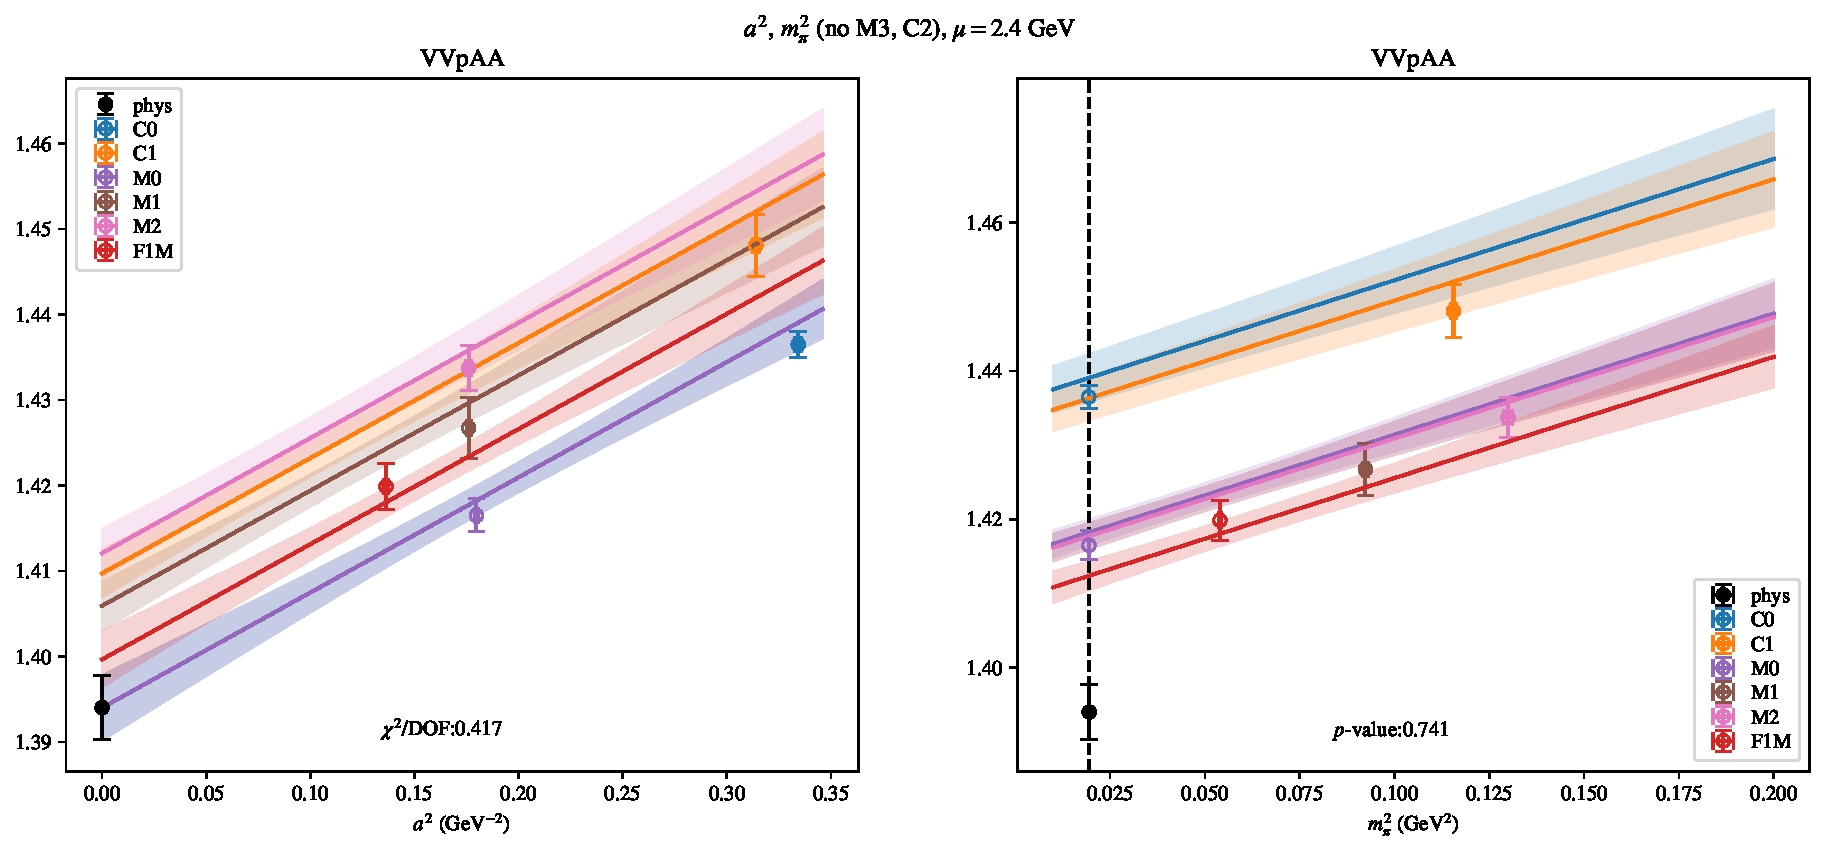
\includepdf[link, pages=-]{VVpAA/SUSY/a2m2mcut_24.pdf}
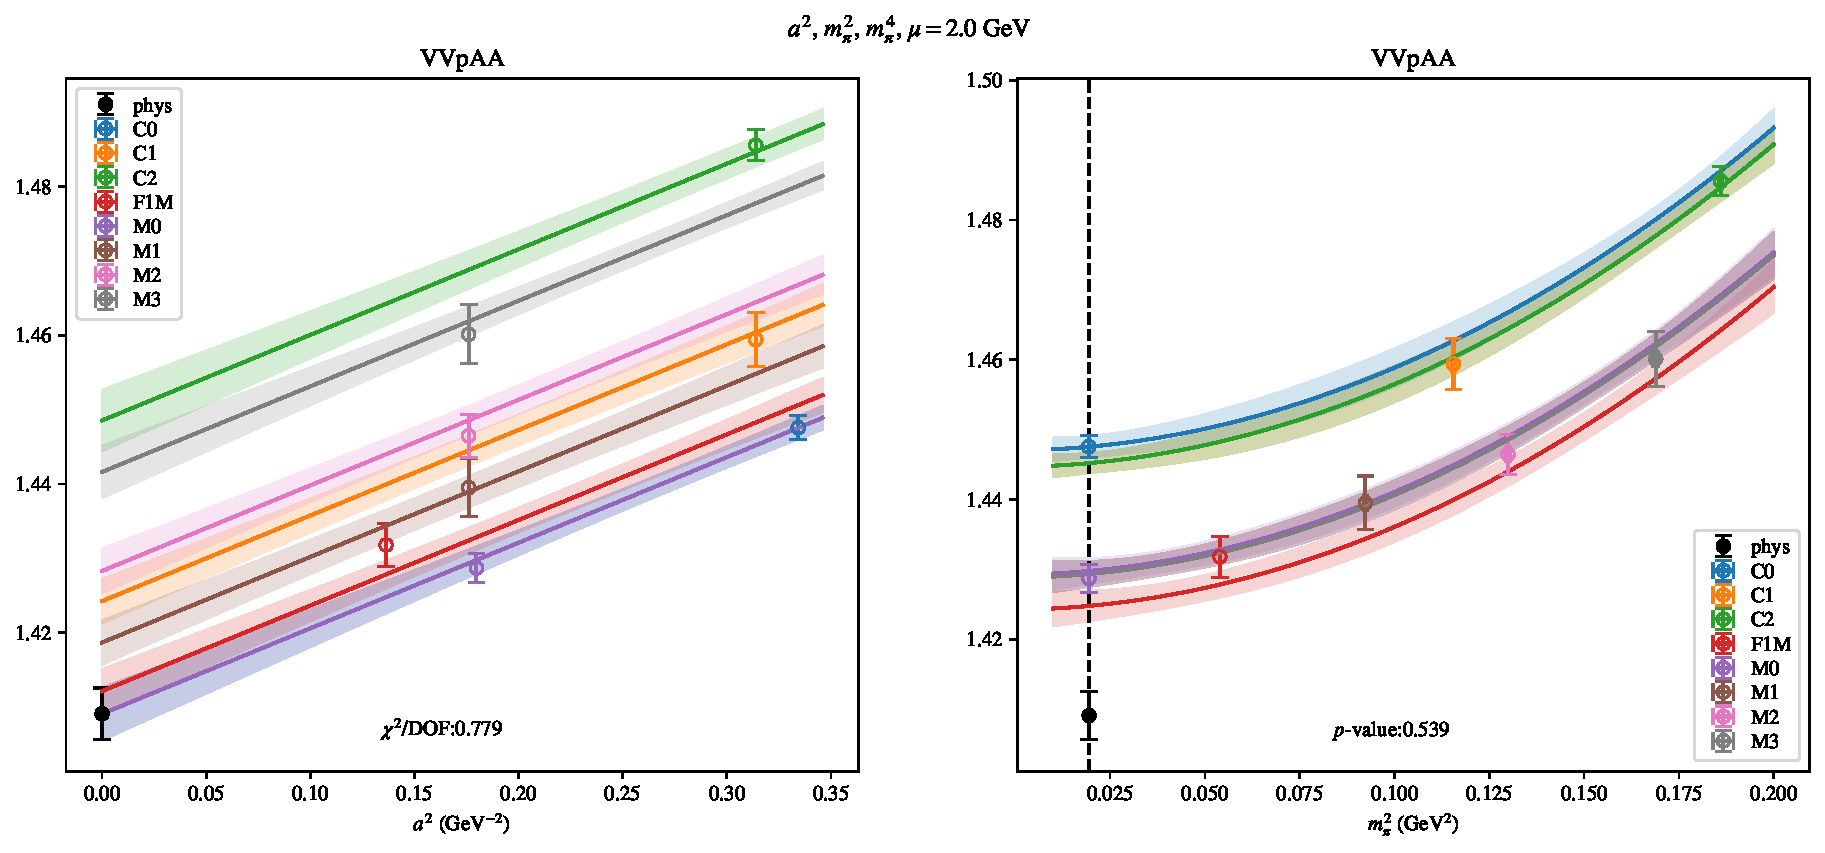
\includepdf[link, pages=-]{VVpAA/SUSY/a2m2m4_20.pdf}
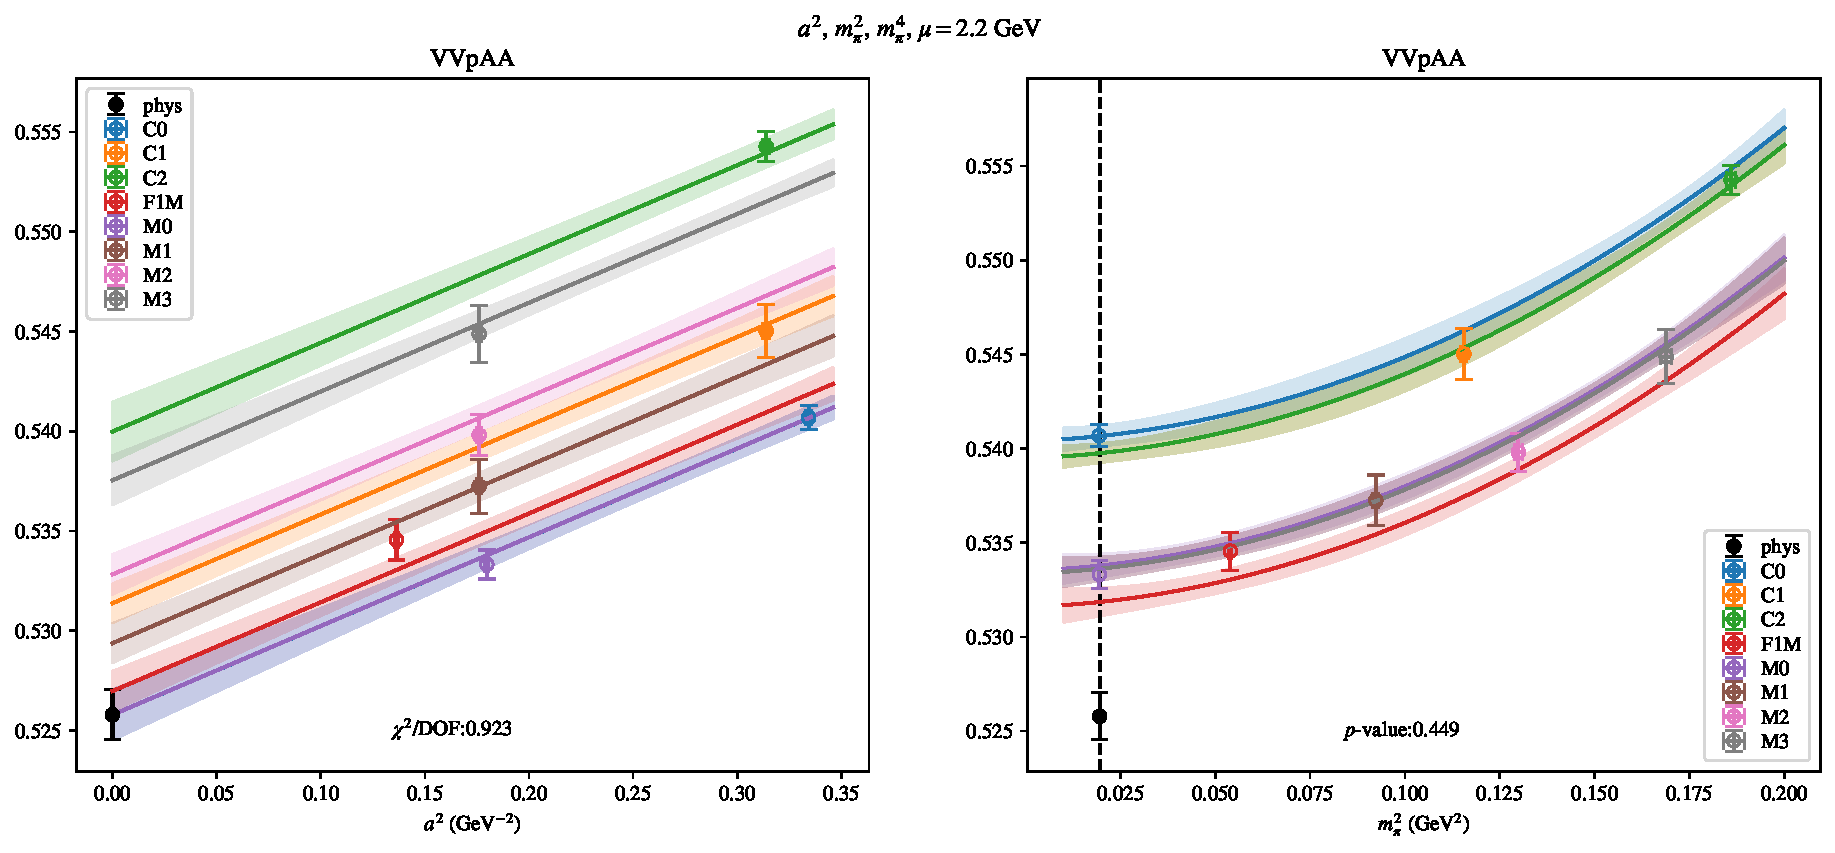
\includepdf[link, pages=-]{VVpAA/SUSY/a2m2m4_22.pdf}
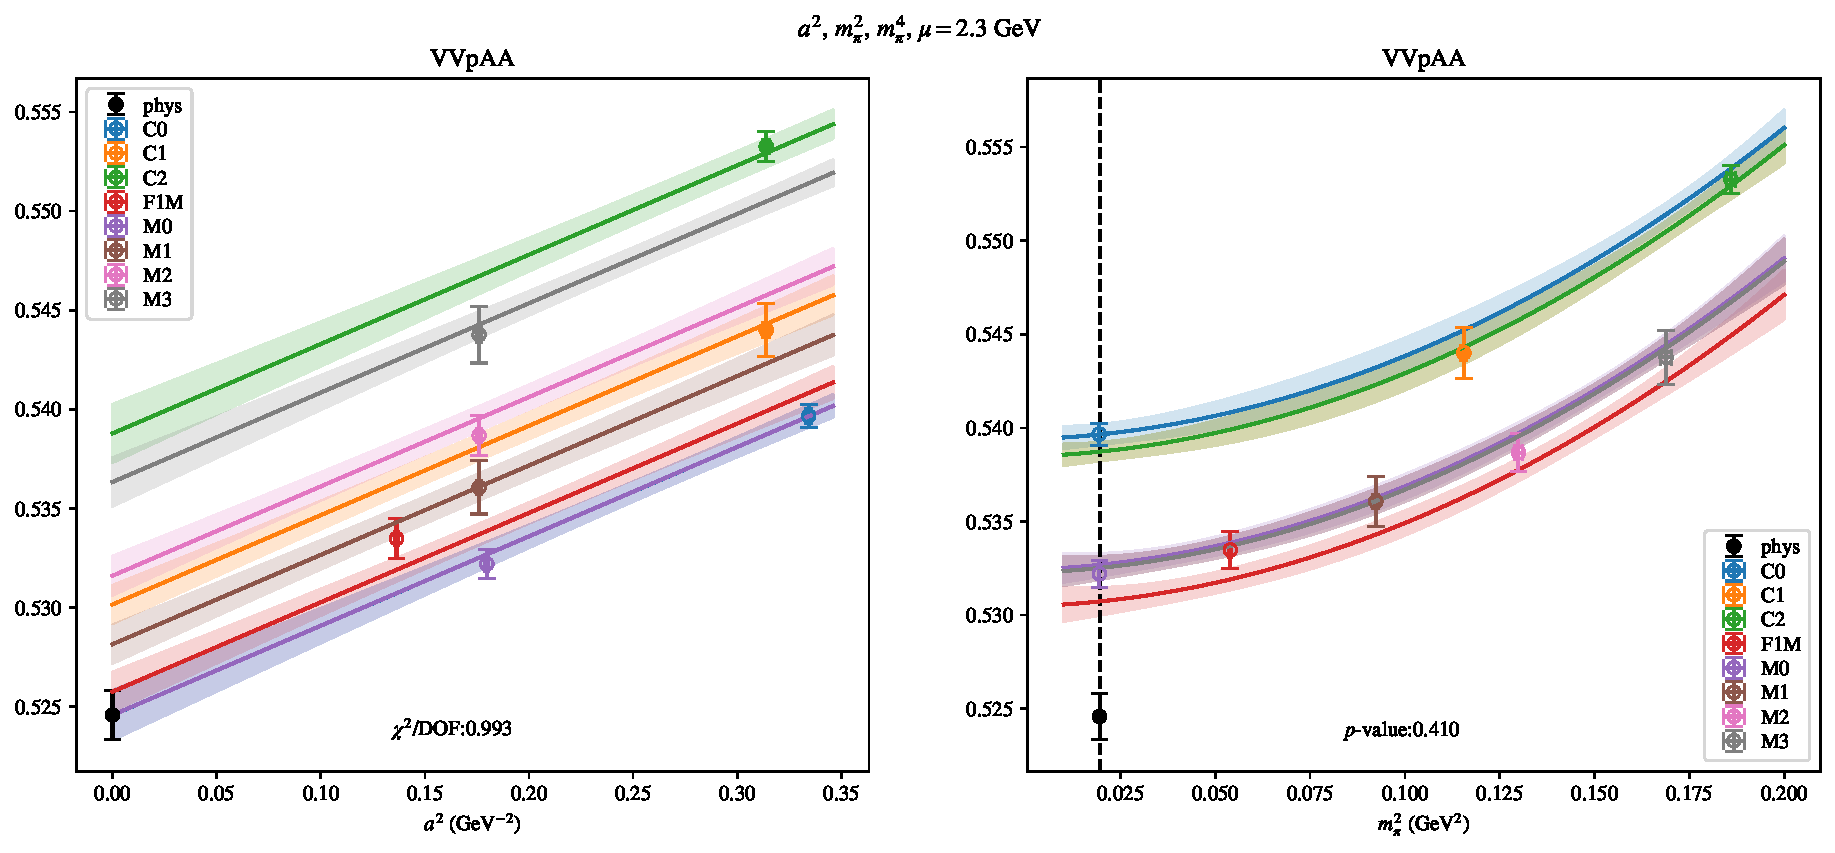
\includepdf[link, pages=-]{VVpAA/SUSY/a2m2m4_23.pdf}
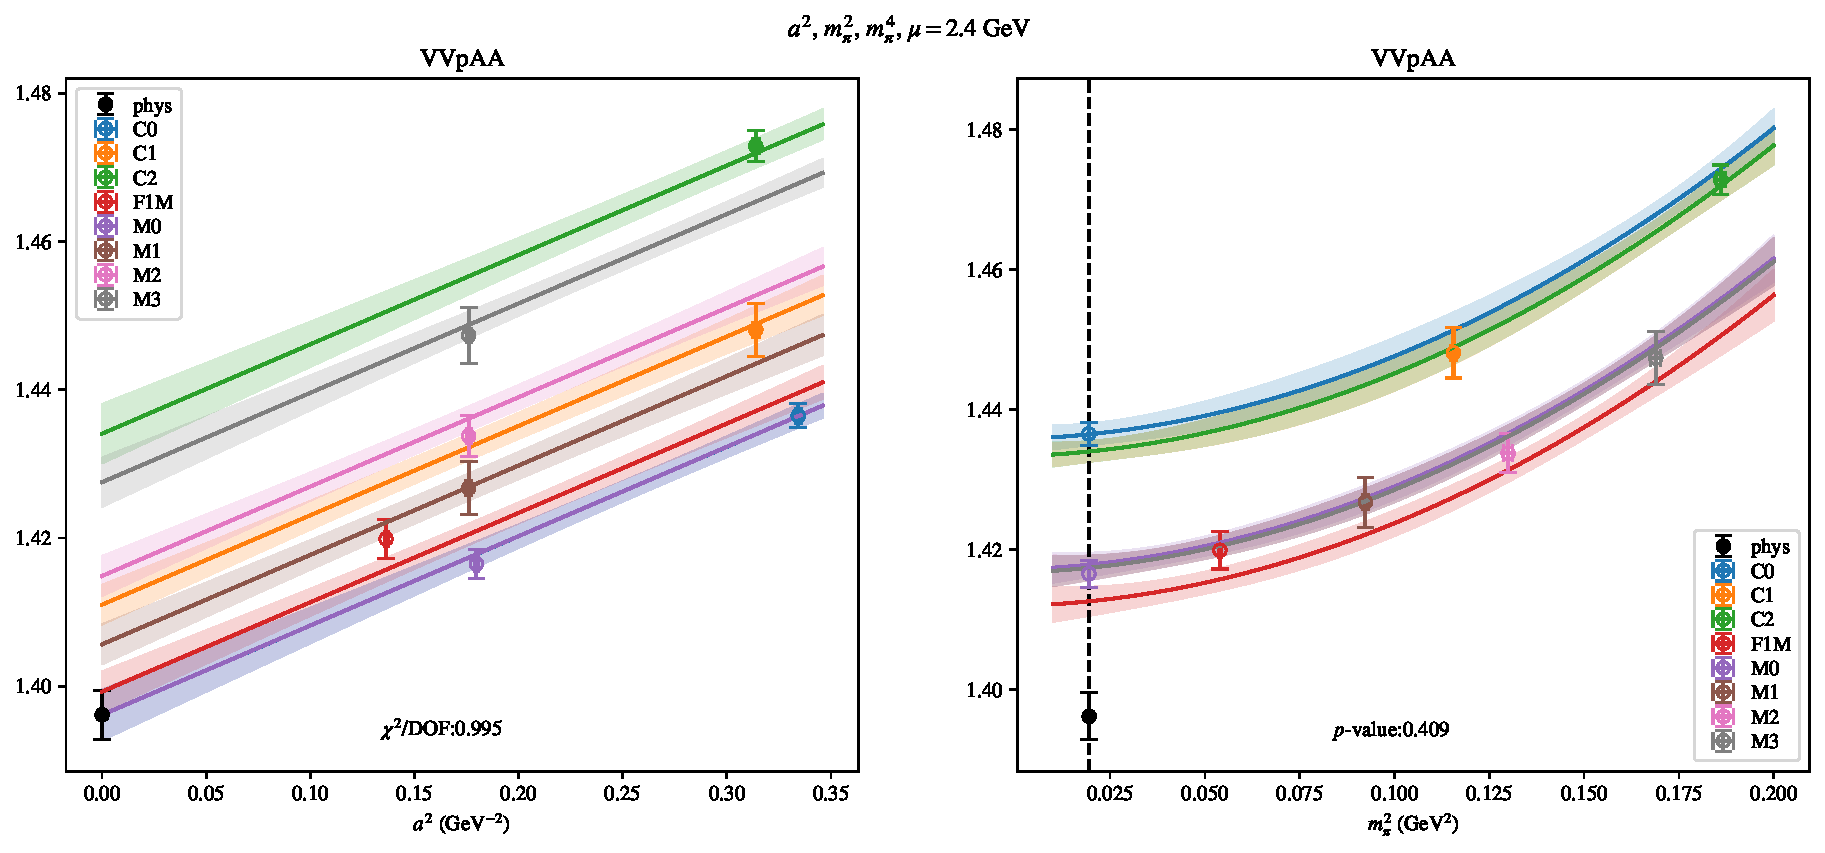
\includepdf[link, pages=-]{VVpAA/SUSY/a2m2m4_24.pdf}
\clearpage
\section{$\mathcal{B}_2$}
\begin{table}[h!]
\begin{center}
\begin{tabular}{|c|c|c|c|c|c|}
\hline
$\mu$ (GeV) & $a^2$, $m_\pi^2$& $a^2$, $m_\pi^2$ (no C)& $a^2$, $a^4$, $m_\pi^2$& $a^2$, $m_\pi^2$ (no M3, C2)& $a^2$, $m_\pi^2$, $m_\pi^4$\\
\hline
2.0& \hyperlink{VVmAA/SUSY/a2m2_20.pdf.1}{\textbf{-0.945(16)}: 8.034 (0.0)} & \hyperlink{VVmAA/SUSY/a2m2noC_20.pdf.1}{\textbf{-0.990(92)}: 2.564 (0.077)} & \hyperlink{VVmAA/SUSY/a2a4m2_20.pdf.1}{\textbf{-0.98(15)}: 7.916 (0.0)} & \hyperlink{VVmAA/SUSY/a2m2mcut_20.pdf.1}{\textbf{-0.945(17)}: 10.158 (0.0)} & \hyperlink{VVmAA/SUSY/a2m2m4_20.pdf.1}{\textbf{-0.943(17)}: 7.375 (0.0)}\\
2.2& \hyperlink{VVmAA/SUSY/a2m2_22.pdf.1}{\textbf{-0.918(15)}: 7.565 (0.0)} & \hyperlink{VVmAA/SUSY/a2m2noC_22.pdf.1}{\textbf{-0.957(89)}: 2.536 (0.079)} & \hyperlink{VVmAA/SUSY/a2a4m2_22.pdf.1}{\textbf{-0.95(14)}: 7.908 (0.0)} & \hyperlink{VVmAA/SUSY/a2m2mcut_22.pdf.1}{\textbf{-0.919(16)}: 9.497 (0.0)} & \hyperlink{VVmAA/SUSY/a2m2m4_22.pdf.1}{\textbf{-0.916(16)}: 7.328 (0.0)}\\
2.3& \hyperlink{VVmAA/SUSY/a2m2_23.pdf.1}{\textbf{-0.907(14)}: 7.131 (0.0)} & \hyperlink{VVmAA/SUSY/a2m2noC_23.pdf.1}{\textbf{-0.945(88)}: 2.476 (0.084)} & \hyperlink{VVmAA/SUSY/a2a4m2_23.pdf.1}{\textbf{-0.94(14)}: 7.297 (0.0)} & \hyperlink{VVmAA/SUSY/a2m2mcut_23.pdf.1}{\textbf{-0.907(16)}: 9.052 (0.0)} & \hyperlink{VVmAA/SUSY/a2m2m4_23.pdf.1}{\textbf{-0.905(16)}: 6.883 (0.0)}\\
2.4& \hyperlink{VVmAA/SUSY/a2m2_24.pdf.1}{\textbf{-0.897(14)}: 7.036 (0.0)} & \hyperlink{VVmAA/SUSY/a2m2noC_24.pdf.1}{\textbf{-0.932(87)}: 2.249 (0.105)} & \hyperlink{VVmAA/SUSY/a2a4m2_24.pdf.1}{\textbf{-0.92(14)}: 7.778 (0.0)} & \hyperlink{VVmAA/SUSY/a2m2mcut_24.pdf.1}{\textbf{-0.898(16)}: 8.752 (0.0)} & \hyperlink{VVmAA/SUSY/a2m2m4_24.pdf.1}{\textbf{-0.896(16)}: 7.226 (0.0)}\\
\hline
\end{tabular}
\caption{Physical point value from chiral and continuum extrapolation at renormalisation scale $\mu$. Entries are \textbf{value(error)}: $\chi^2/\text{DOF}$ ($p$-value).}
\end{center}
\end{table}
\begin{table}[h!]
\begin{center}
\begin{tabular}{|c c|c|c|c|c|c|}
\hline
$\mu$ (GeV) &  & $a^2$, $m_\pi^2$& $a^2$, $m_\pi^2$ (no C)& $a^2$, $a^4$, $m_\pi^2$& $a^2$, $m_\pi^2$ (no M3, C2)& $a^2$, $m_\pi^2$, $m_\pi^4$\\
\hline
\multirow{2}{0.5in}{2.0} & $\alpha$ & 0.3828(67)& 0.110(54)& -0.029& 0.3814(73)& 0.3917(73)\\
 & $\beta$ & 0.00764(13)& 0.00678(21)& 0.00744(14)& 0.00812(23)& 0.01013(70)\\
\hline
\multirow{2}{0.5in}{2.2} & $\alpha$ & 0.4217(67)& 0.176(55)& 0.075& 0.4194(74)& 0.4299(74)\\
 & $\beta$ & 0.00760(13)& 0.00675(20)& 0.00743(14)& 0.00800(23)& 0.00978(69)\\
\hline
\multirow{2}{0.5in}{2.3} & $\alpha$ & 0.4432(68)& 0.199(55)& 0.089& 0.4410(75)& 0.4512(75)\\
 & $\beta$ & 0.00756(13)& 0.00675(20)& 0.00739(14)& 0.00795(23)& 0.00969(70)\\
\hline
\multirow{2}{0.5in}{2.4} & $\alpha$ & 0.4607(68)& 0.236(56)& 0.17(14)& 0.4573(75)& 0.4677(75)\\
 & $\beta$ & 0.00757(13)& 0.00670(20)& 0.00744(14)& 0.00791(23)& 0.00945(70)\\
\hline
\end{tabular}
\caption{Fit values of coefficients in $Q = Q_{phys} + \mathbf{\alpha} a^2 + \mathbf{\beta}\left(\frac{m_\pi^2}{f_\pi^2}-\frac{m_{\pi,PDG}^2}{f_\pi^2}\right) + \ldots$.}
\end{center}
\end{table}
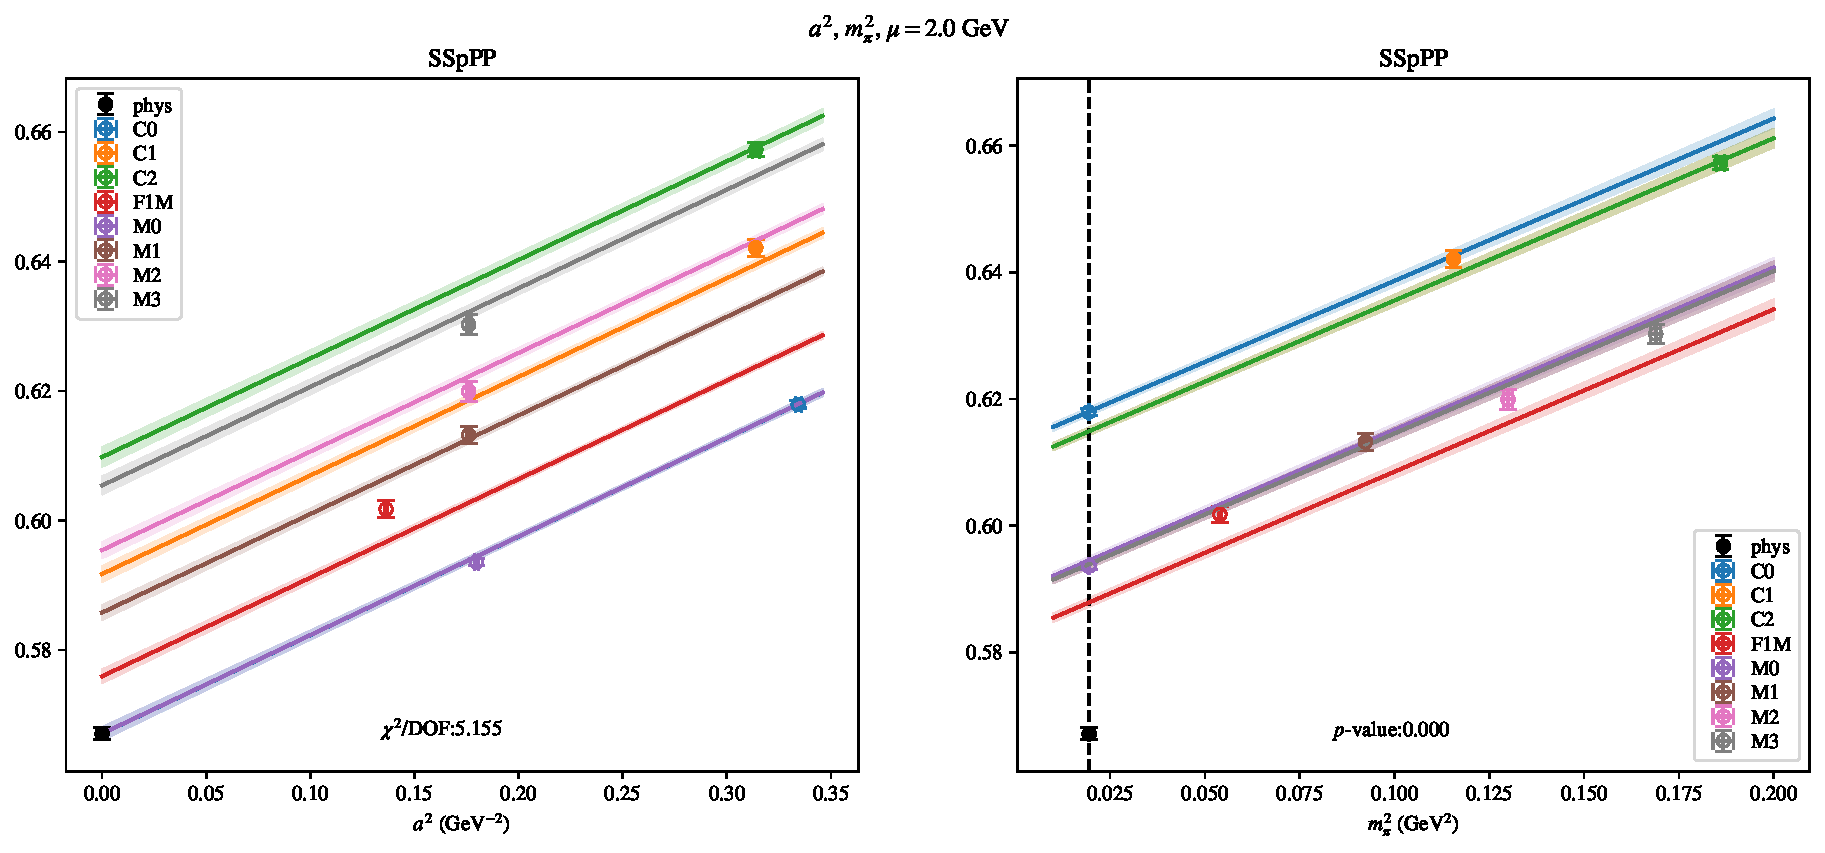
\includepdf[link, pages=-]{VVmAA/SUSY/a2m2_20.pdf}
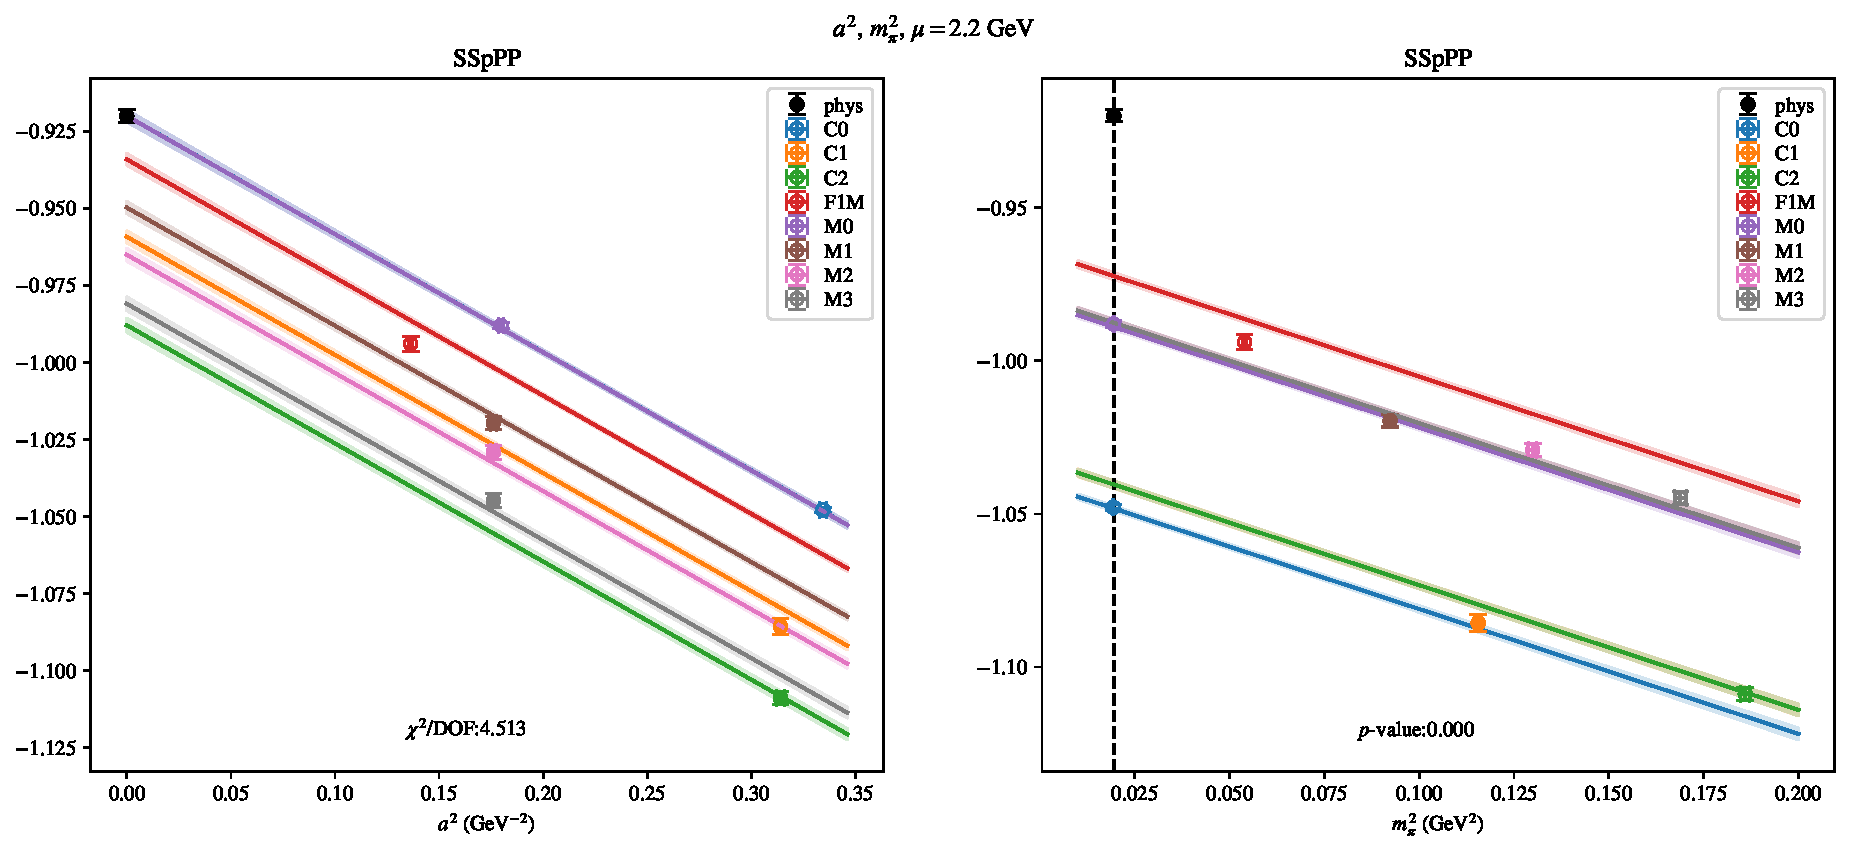
\includepdf[link, pages=-]{VVmAA/SUSY/a2m2_22.pdf}
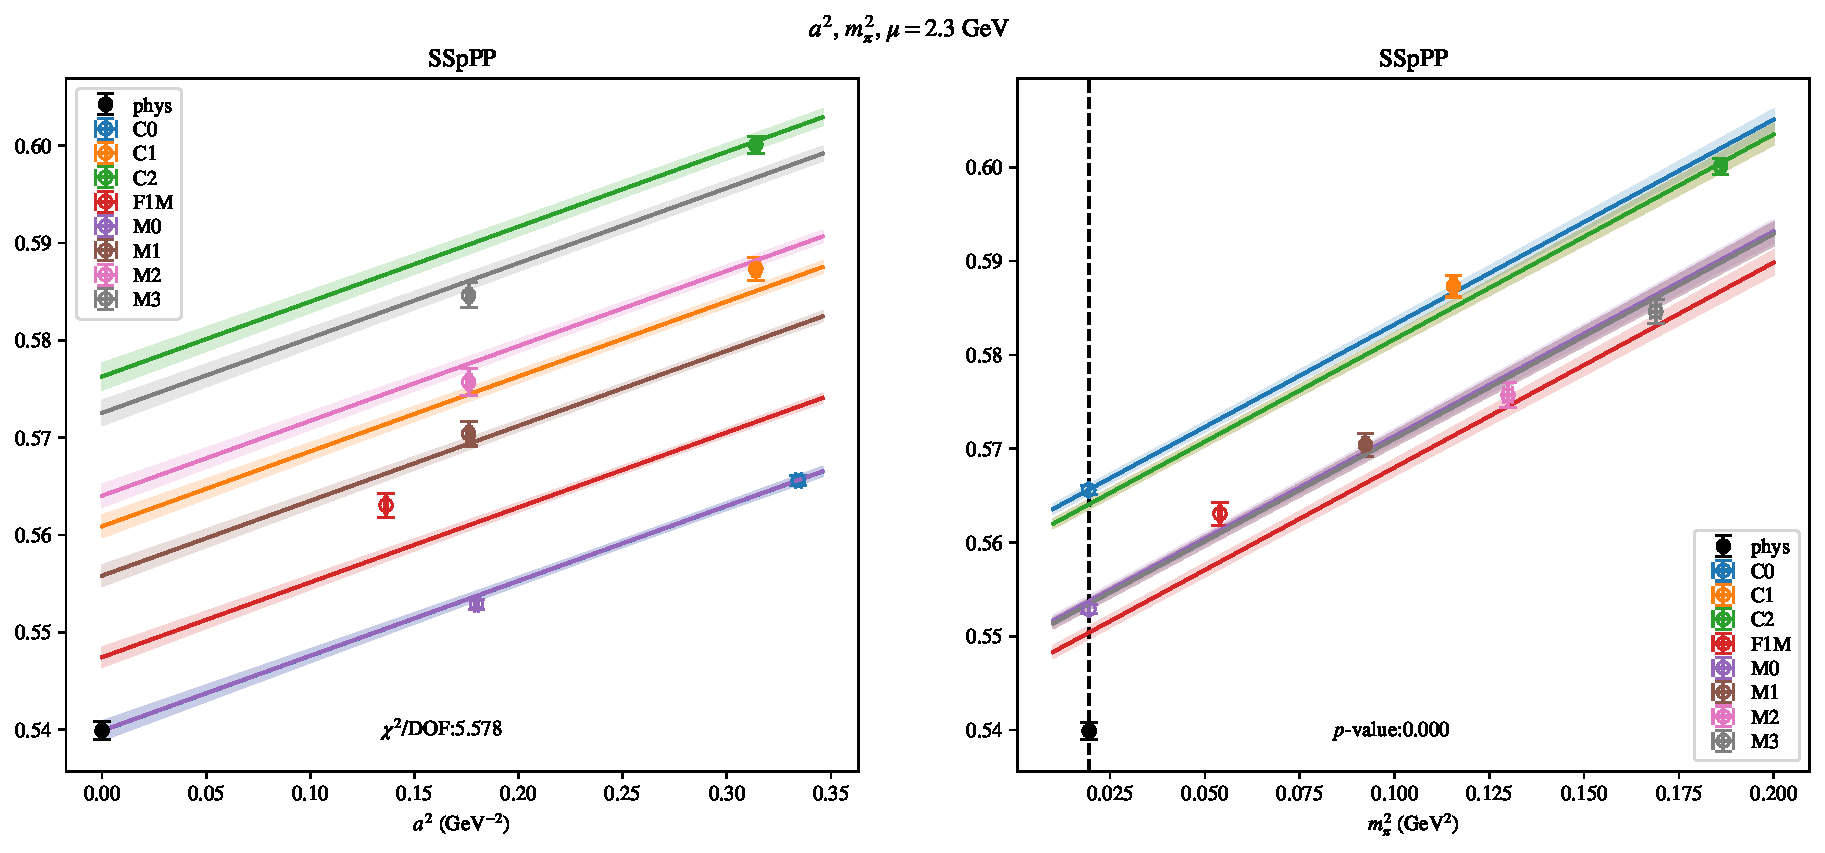
\includepdf[link, pages=-]{VVmAA/SUSY/a2m2_23.pdf}
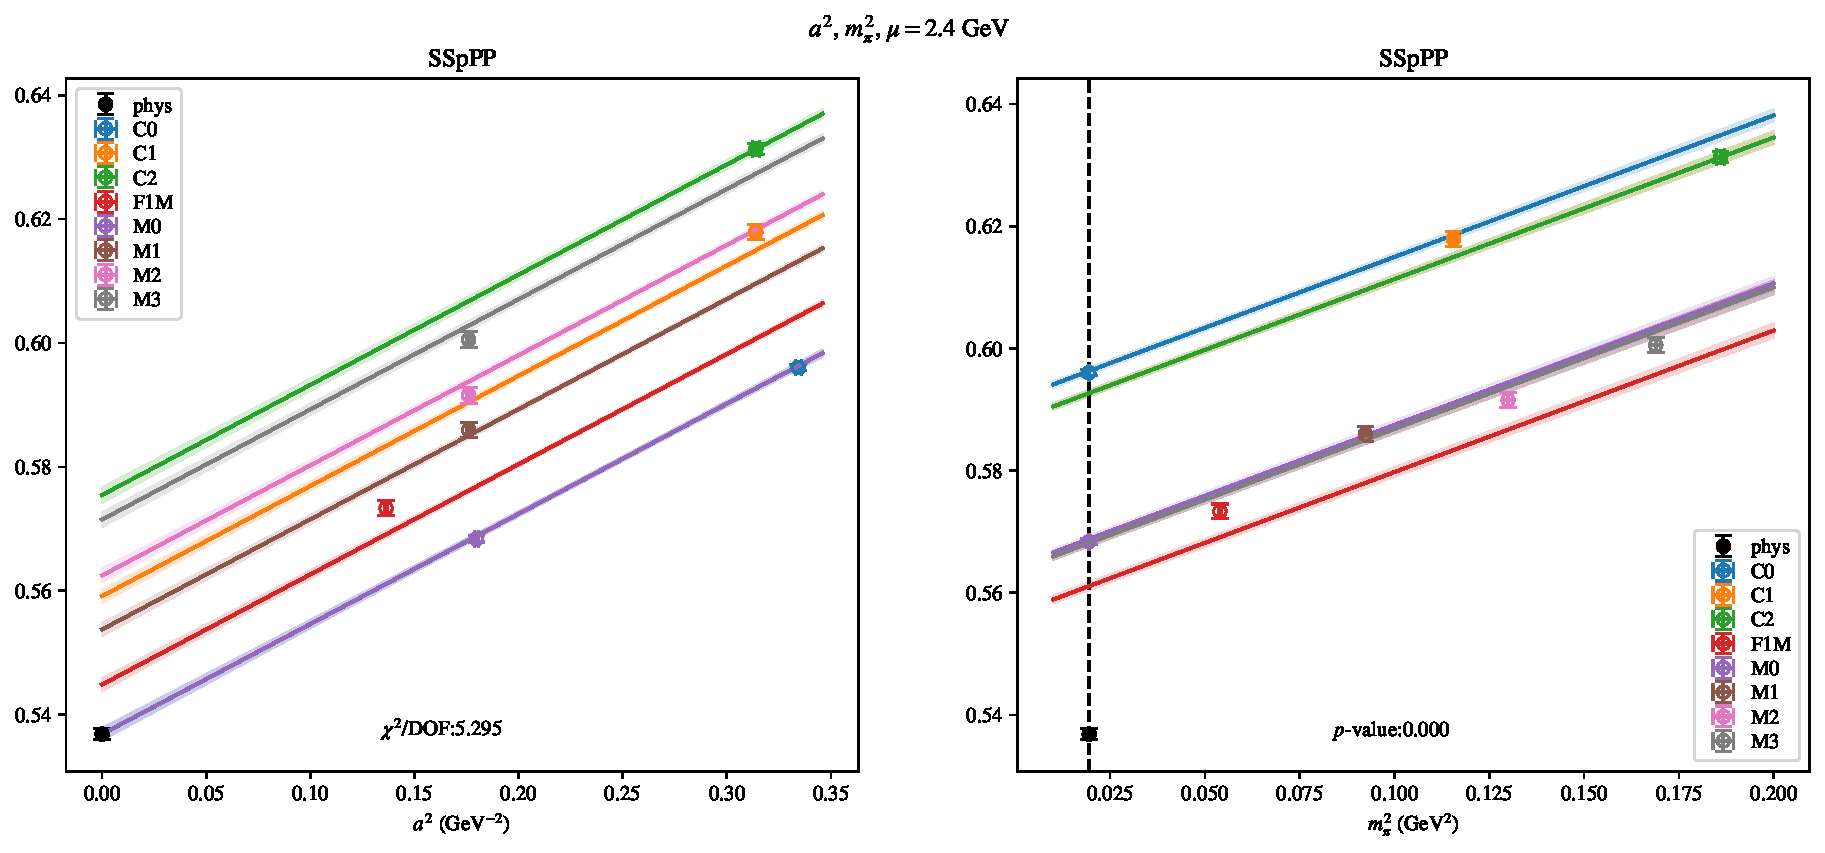
\includepdf[link, pages=-]{VVmAA/SUSY/a2m2_24.pdf}
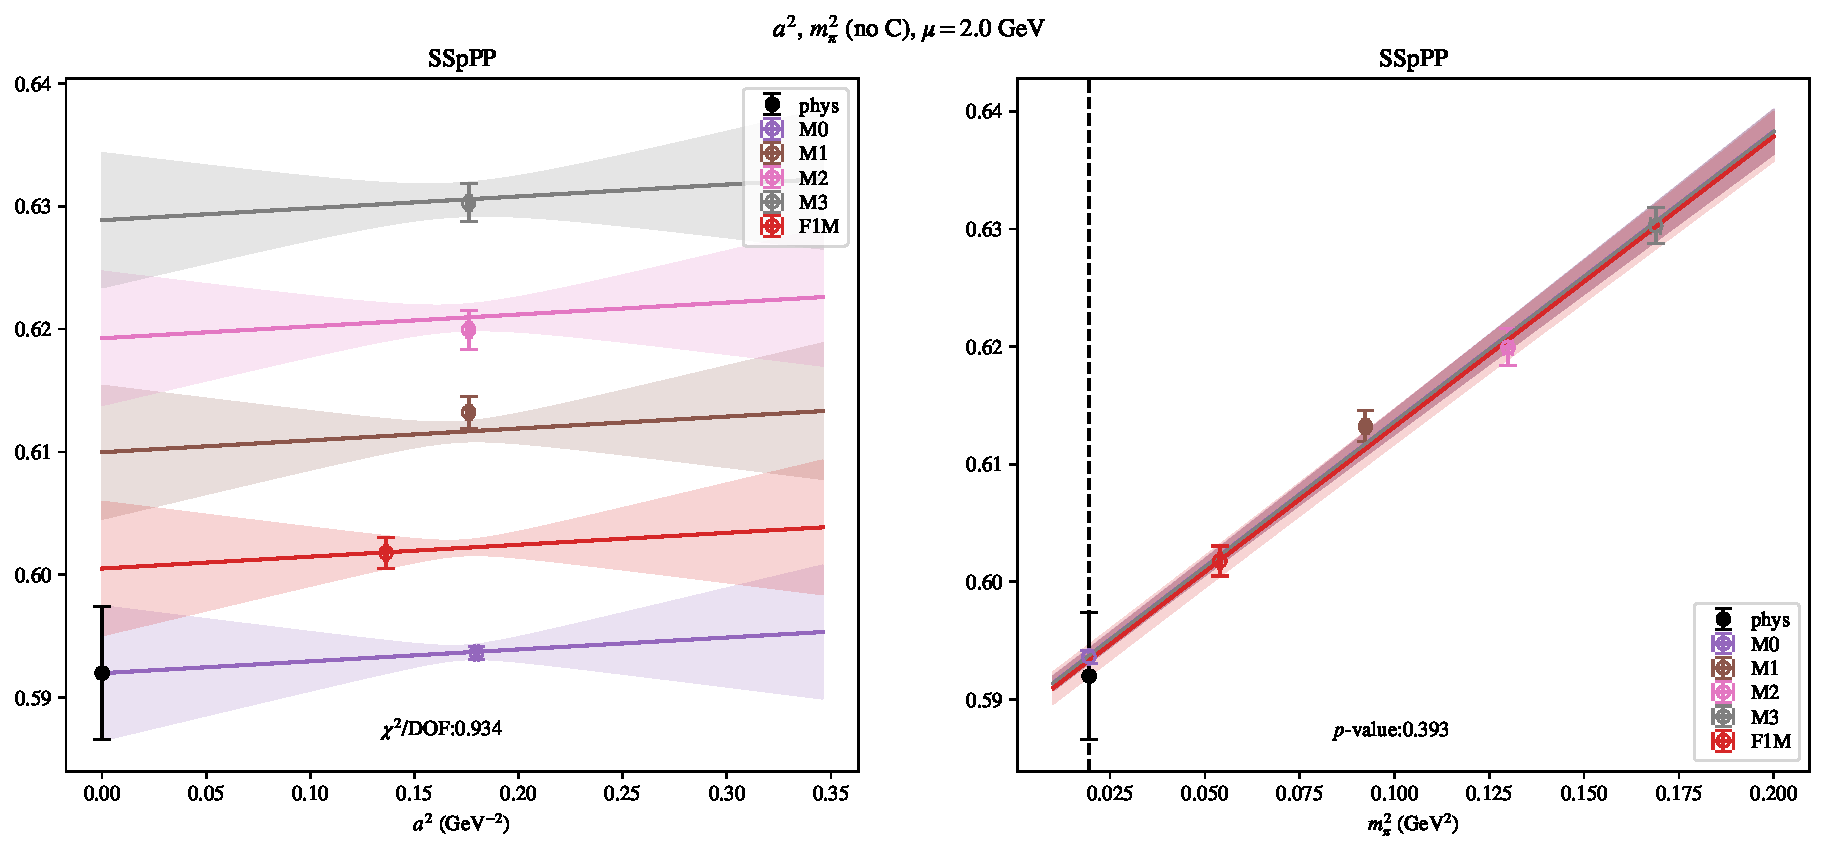
\includepdf[link, pages=-]{VVmAA/SUSY/a2m2noC_20.pdf}
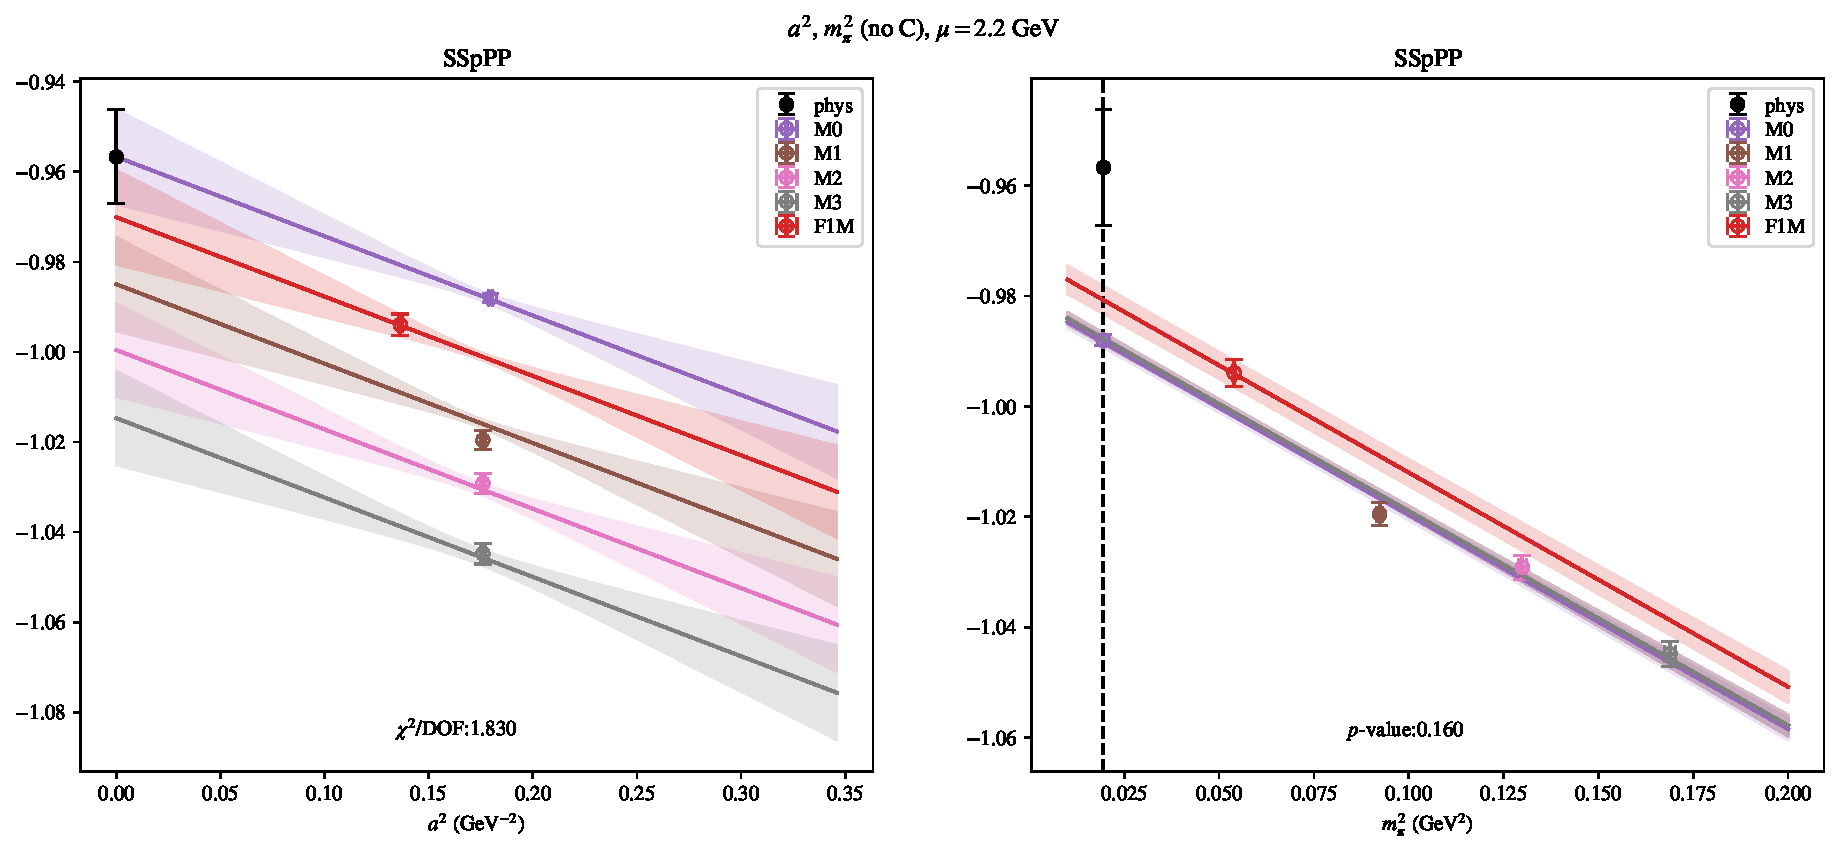
\includepdf[link, pages=-]{VVmAA/SUSY/a2m2noC_22.pdf}
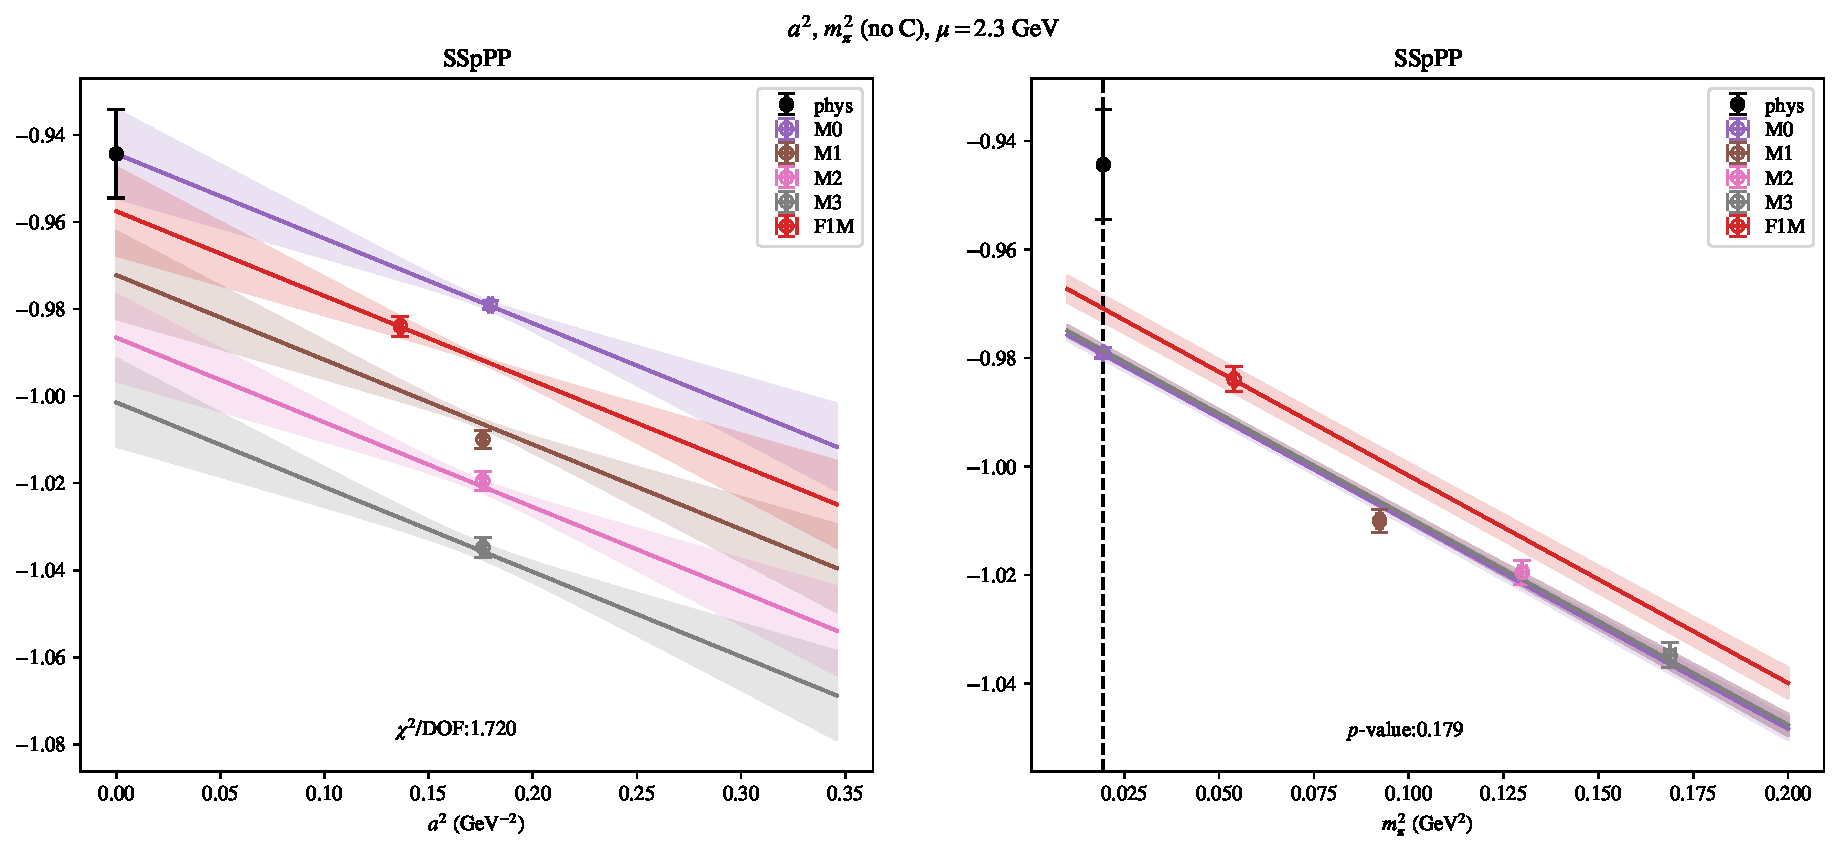
\includepdf[link, pages=-]{VVmAA/SUSY/a2m2noC_23.pdf}
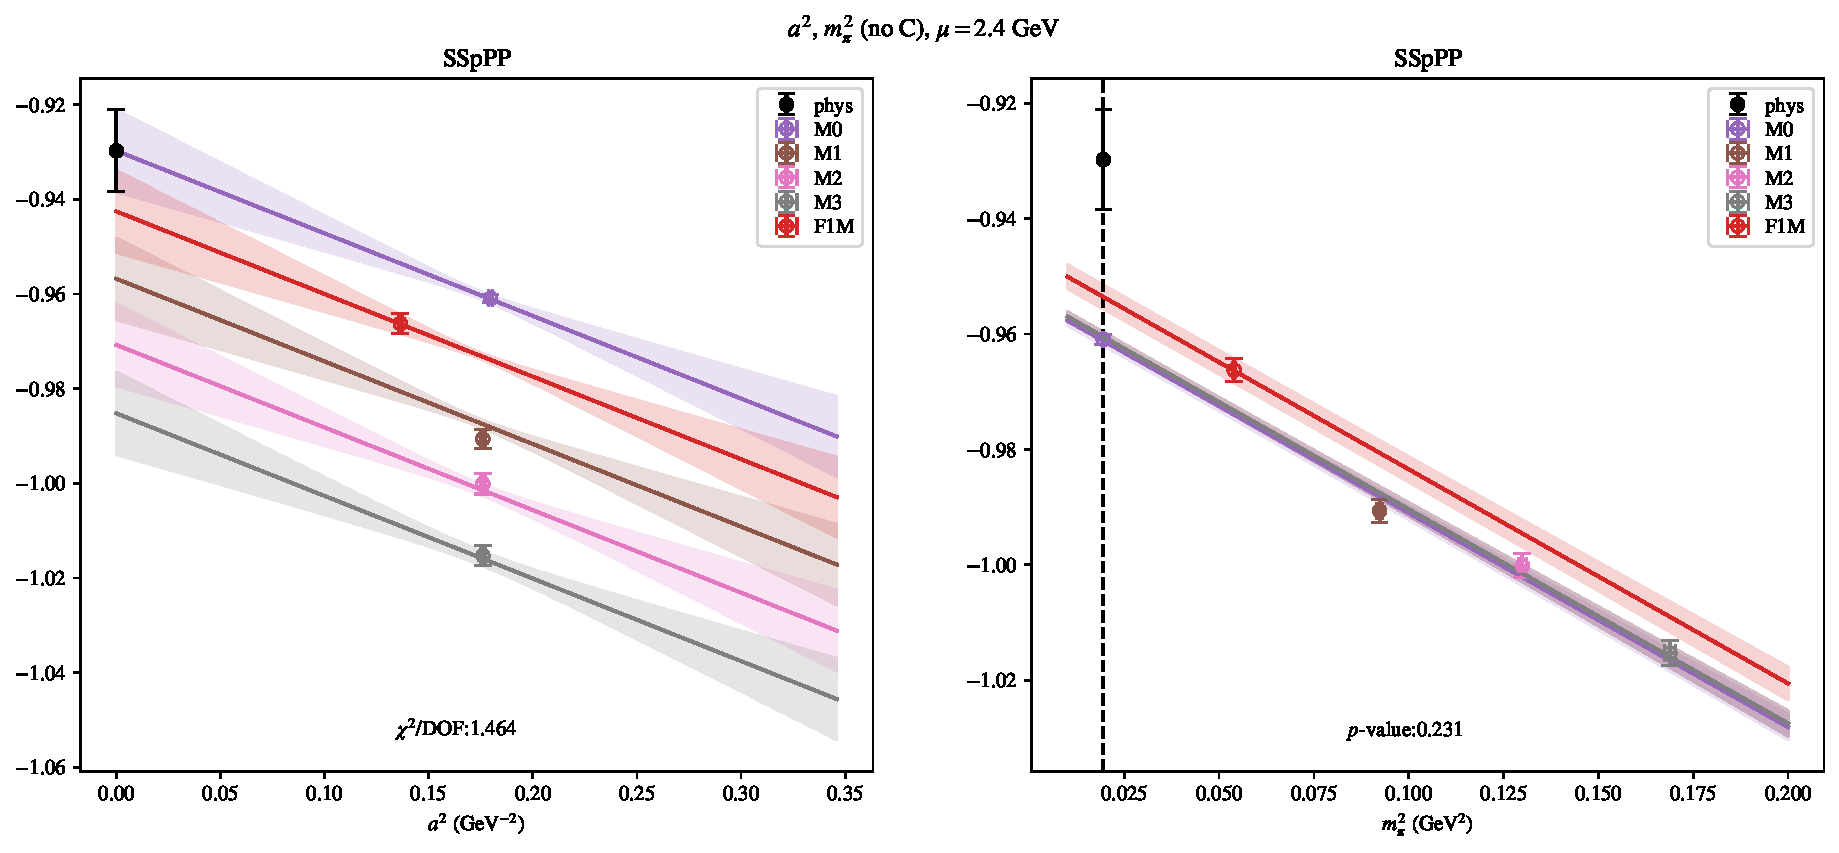
\includepdf[link, pages=-]{VVmAA/SUSY/a2m2noC_24.pdf}
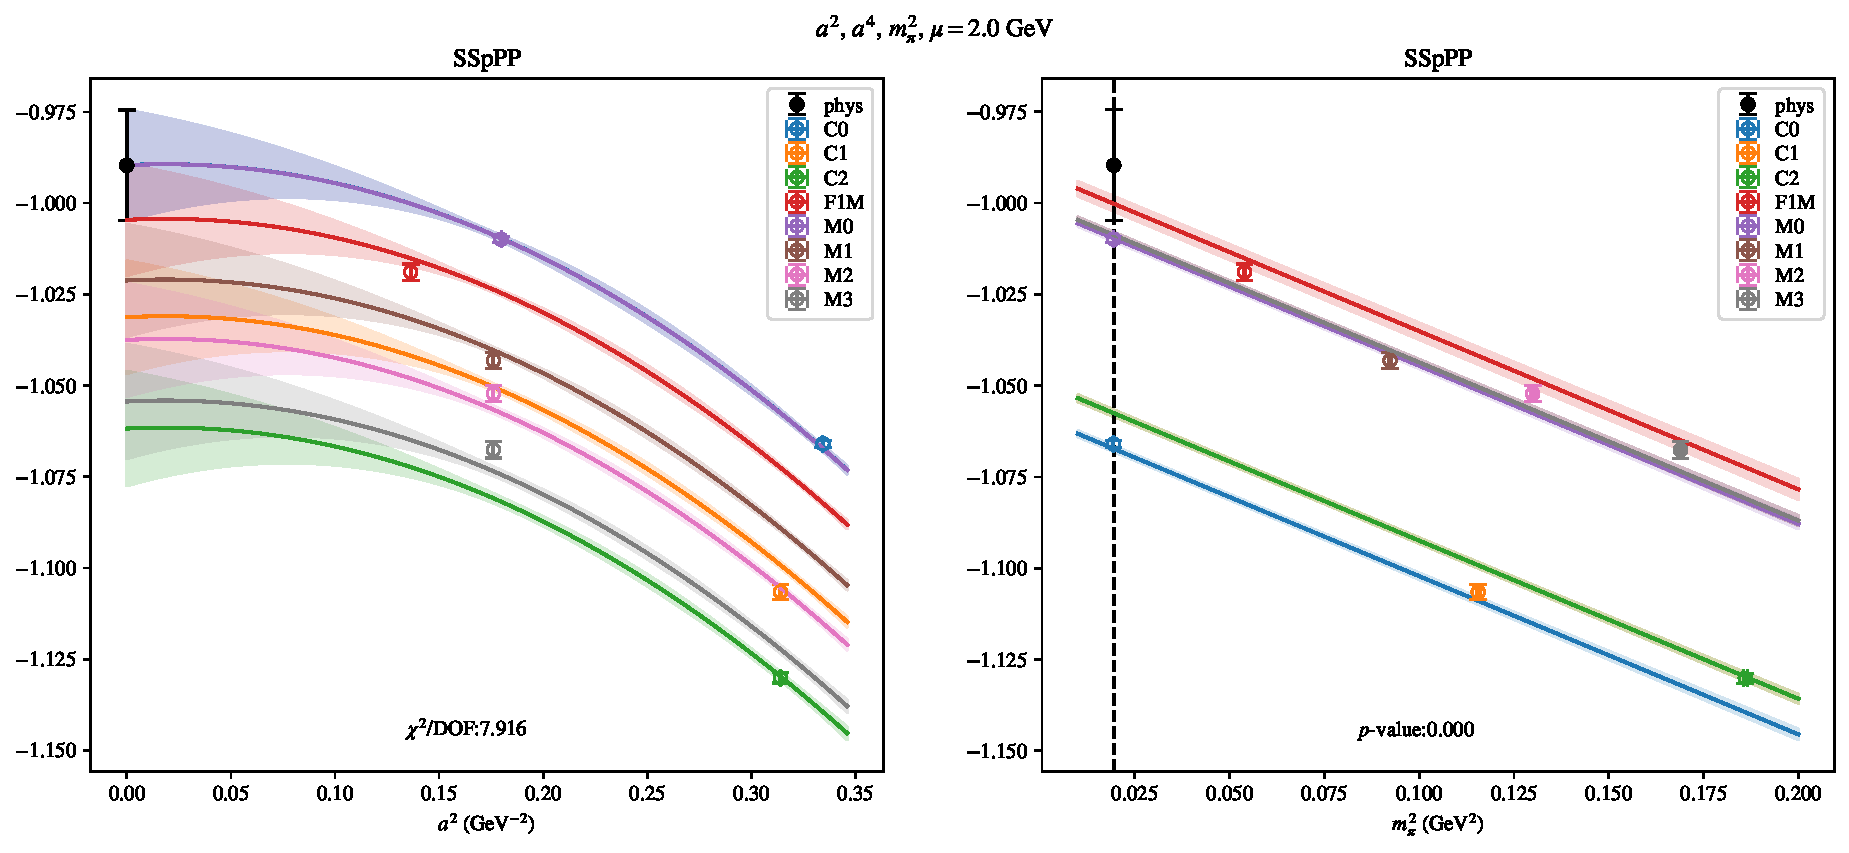
\includepdf[link, pages=-]{VVmAA/SUSY/a2a4m2_20.pdf}
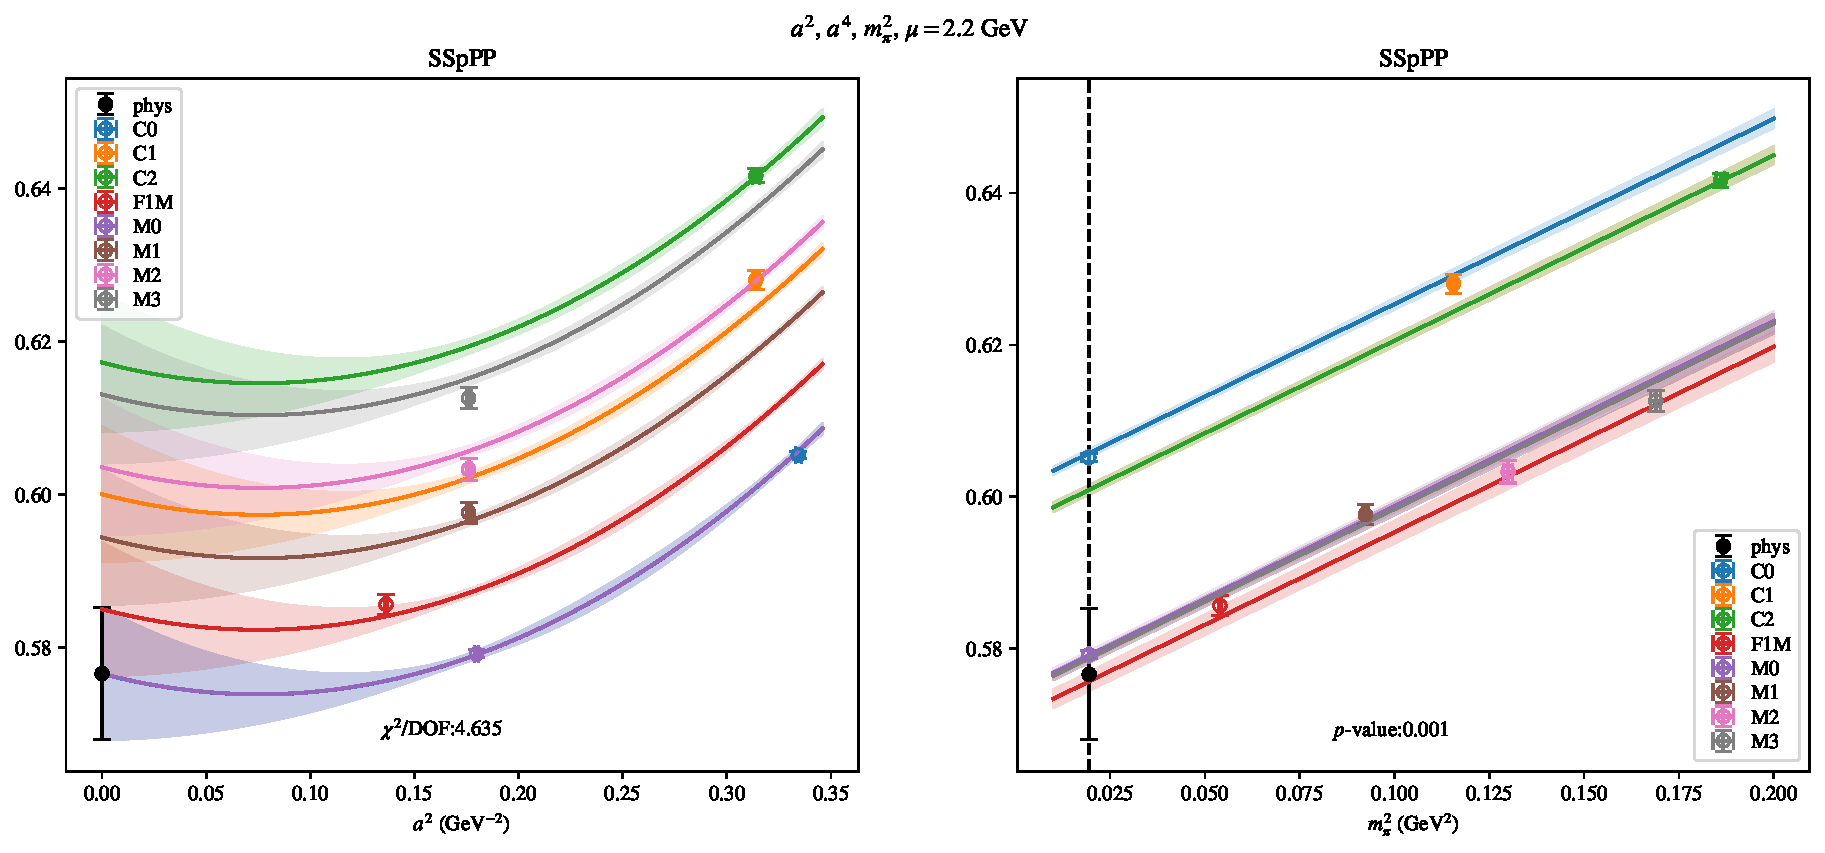
\includepdf[link, pages=-]{VVmAA/SUSY/a2a4m2_22.pdf}
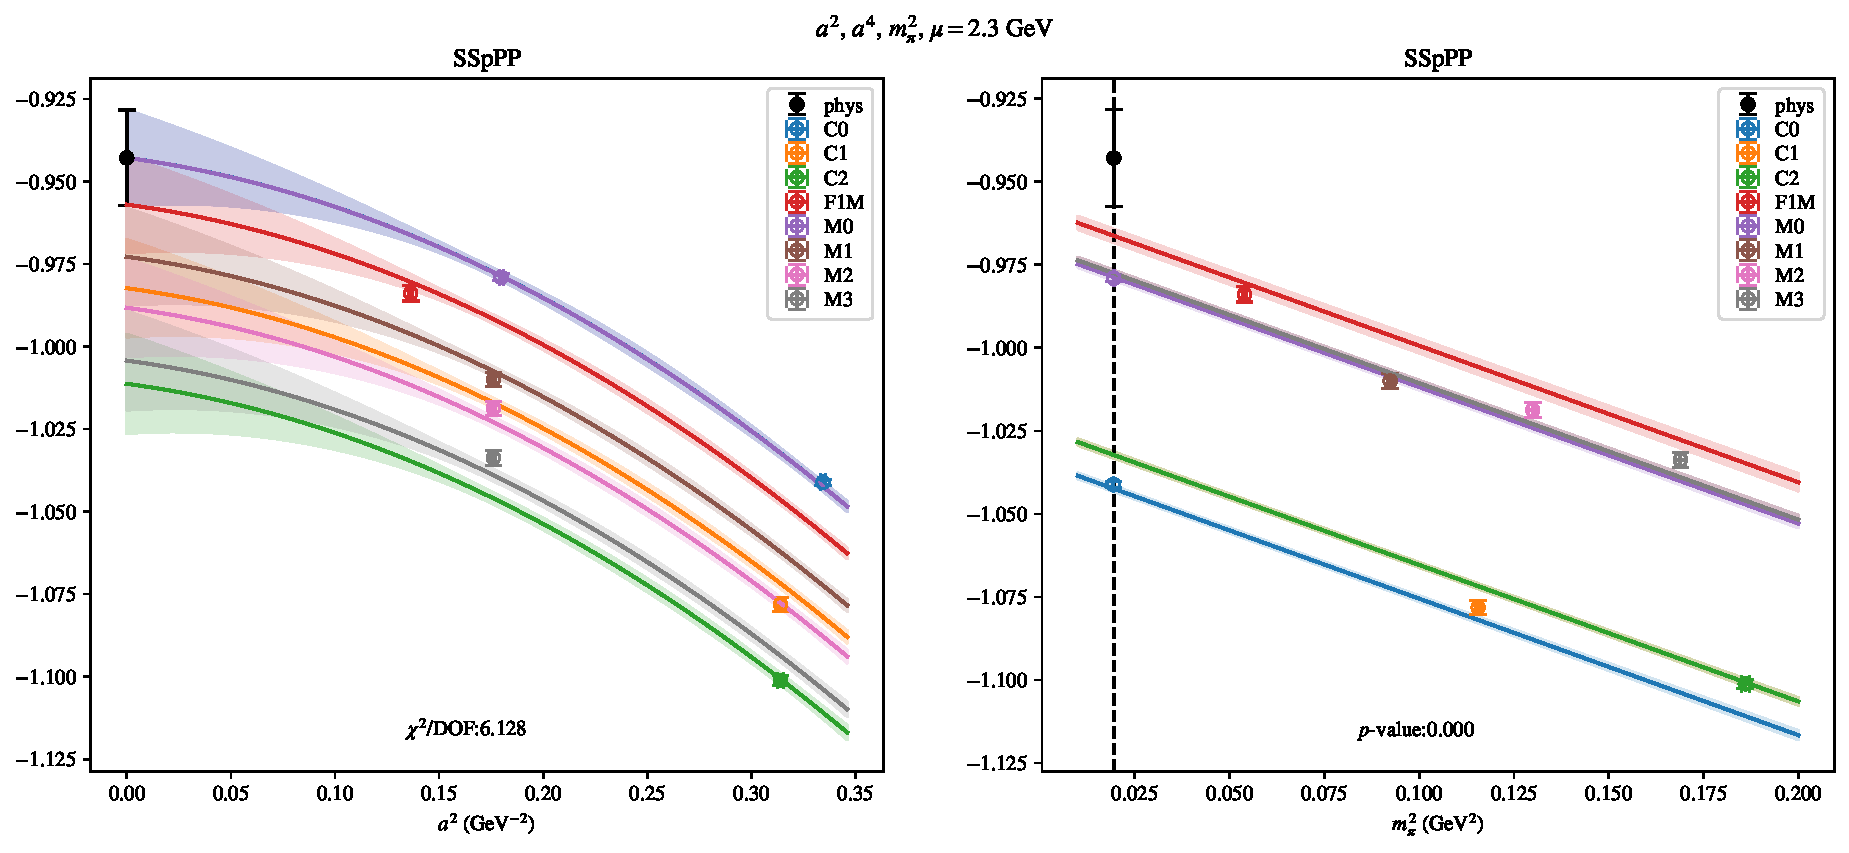
\includepdf[link, pages=-]{VVmAA/SUSY/a2a4m2_23.pdf}
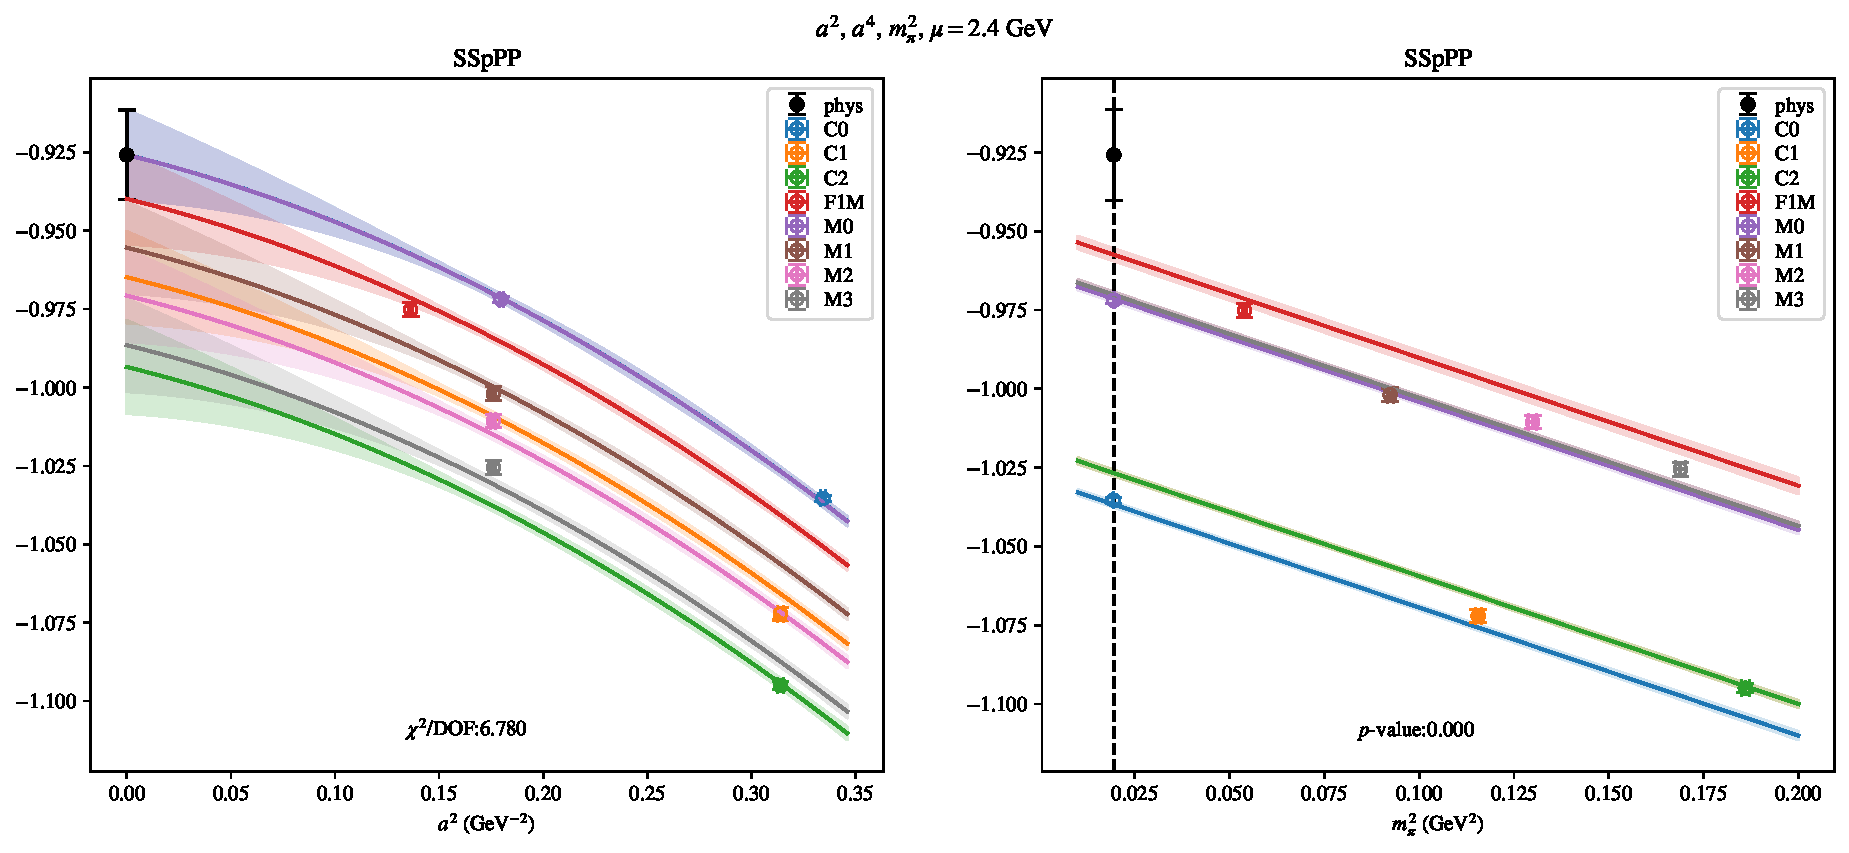
\includepdf[link, pages=-]{VVmAA/SUSY/a2a4m2_24.pdf}
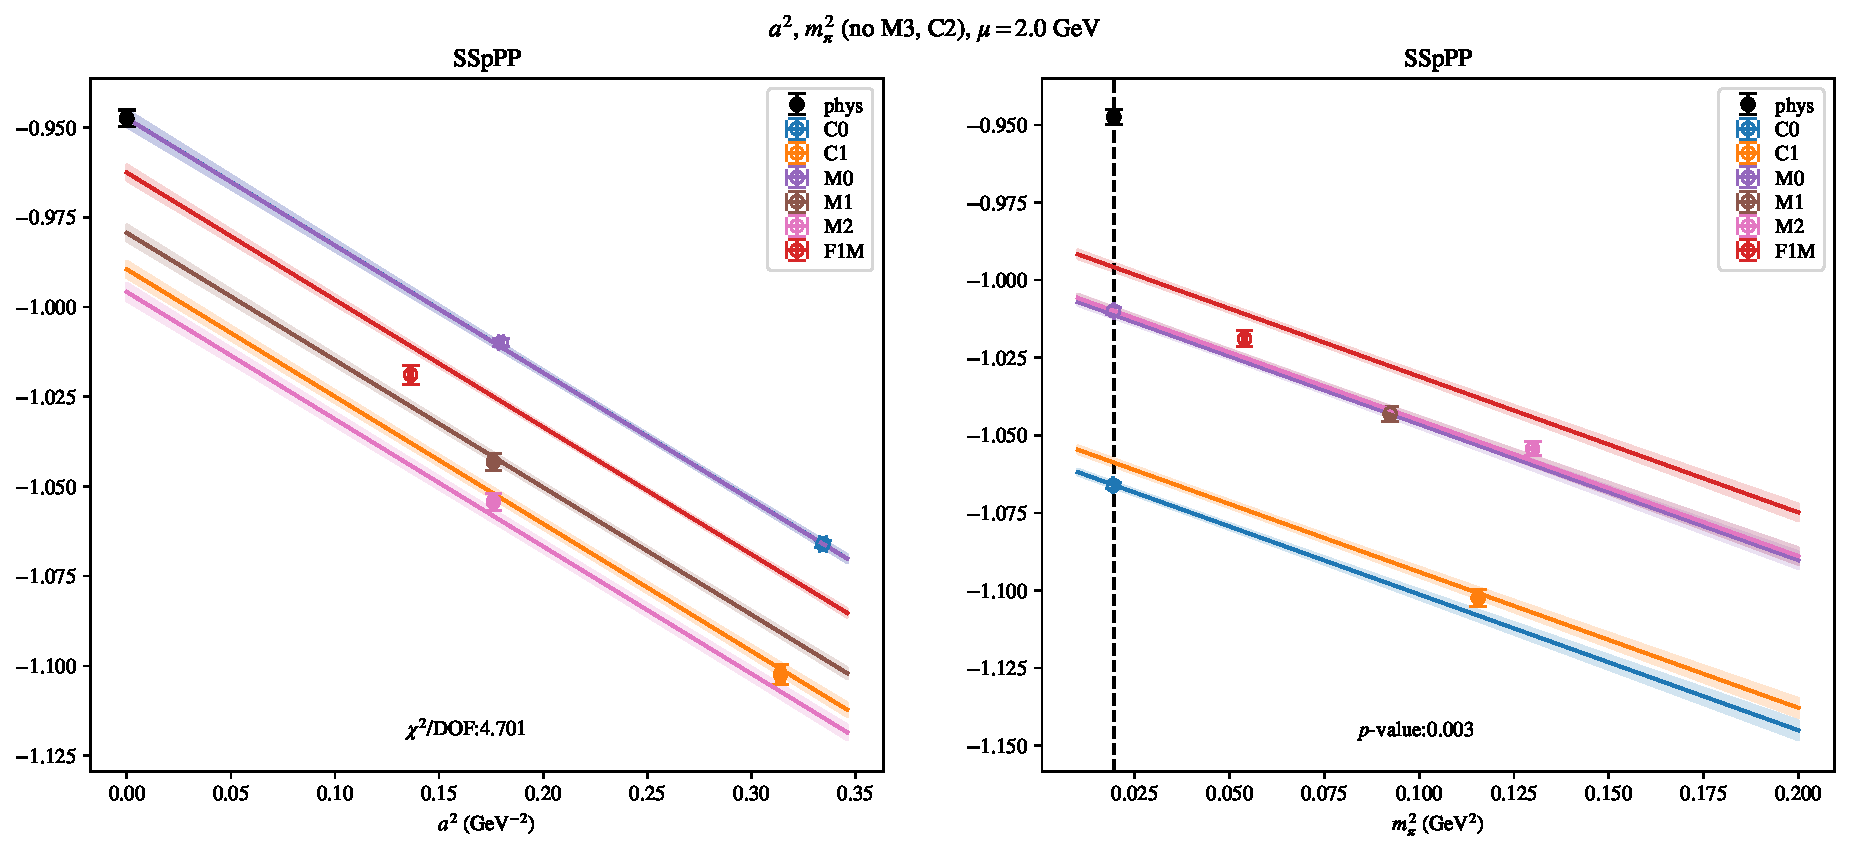
\includepdf[link, pages=-]{VVmAA/SUSY/a2m2mcut_20.pdf}
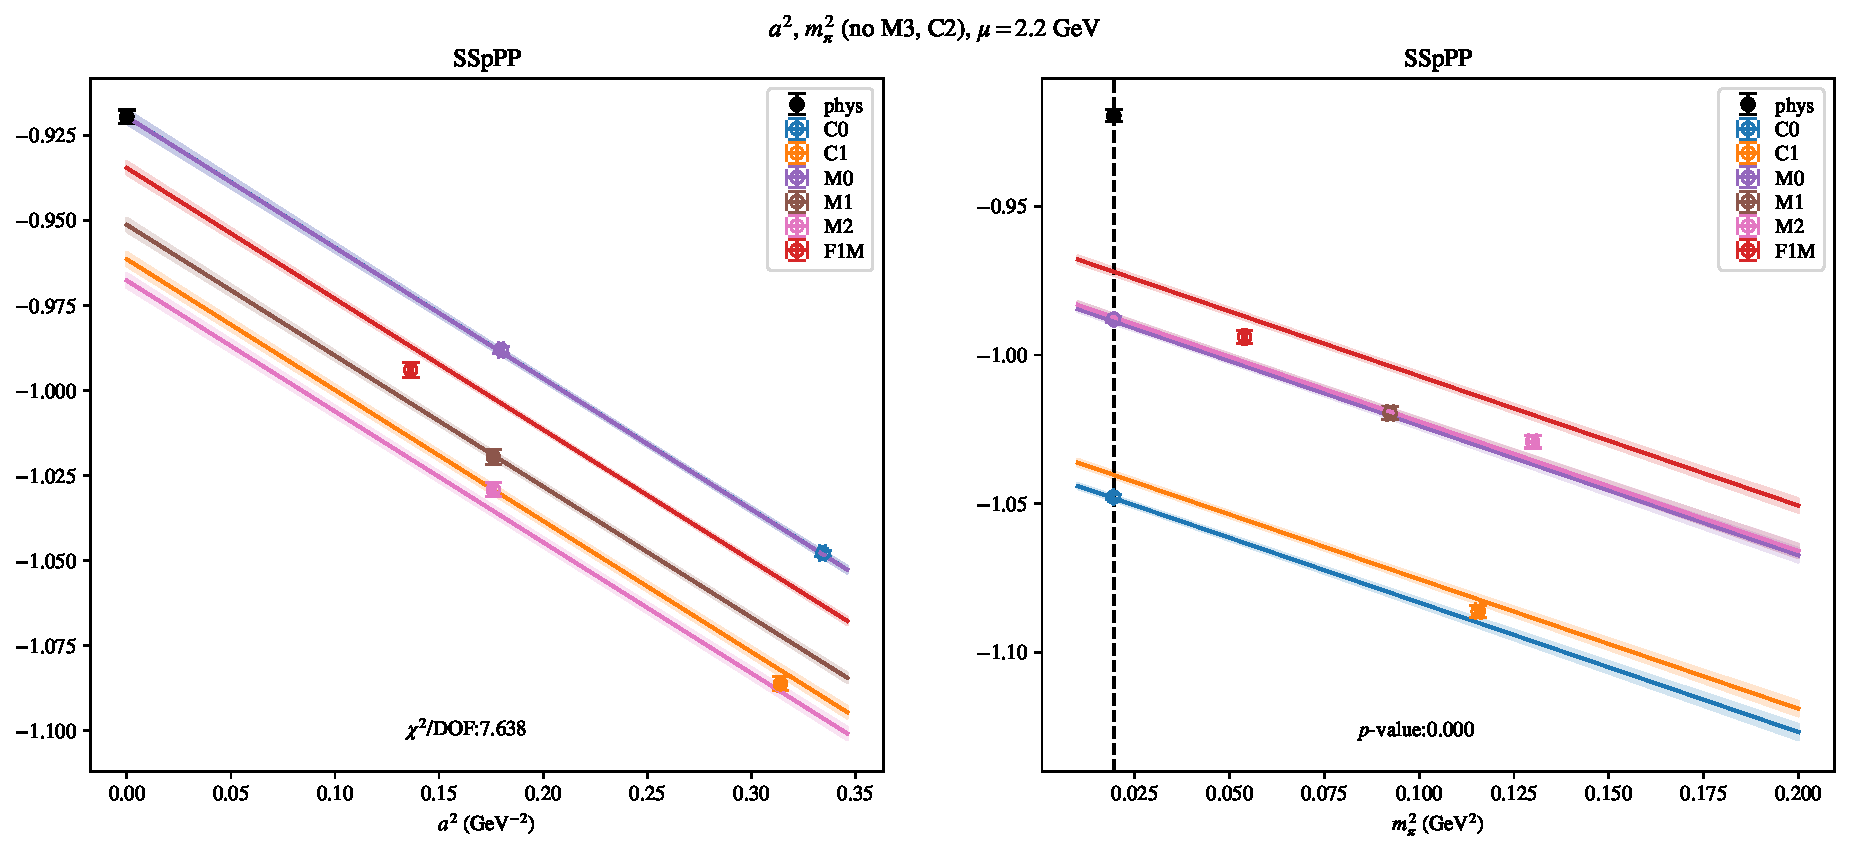
\includepdf[link, pages=-]{VVmAA/SUSY/a2m2mcut_22.pdf}
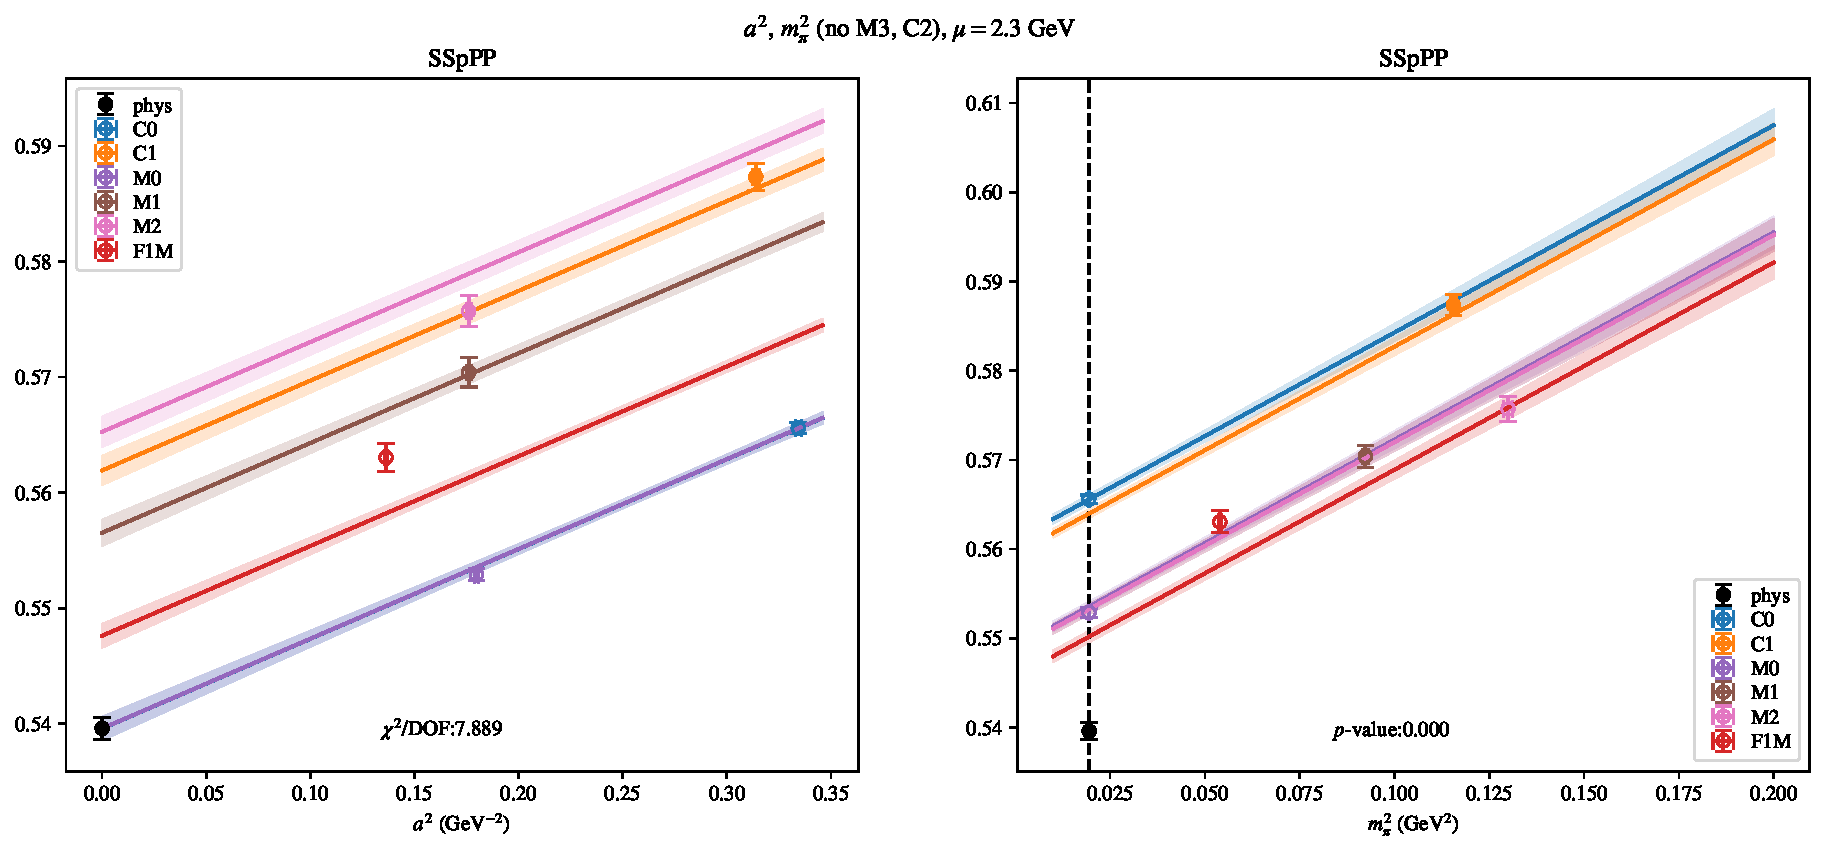
\includepdf[link, pages=-]{VVmAA/SUSY/a2m2mcut_23.pdf}
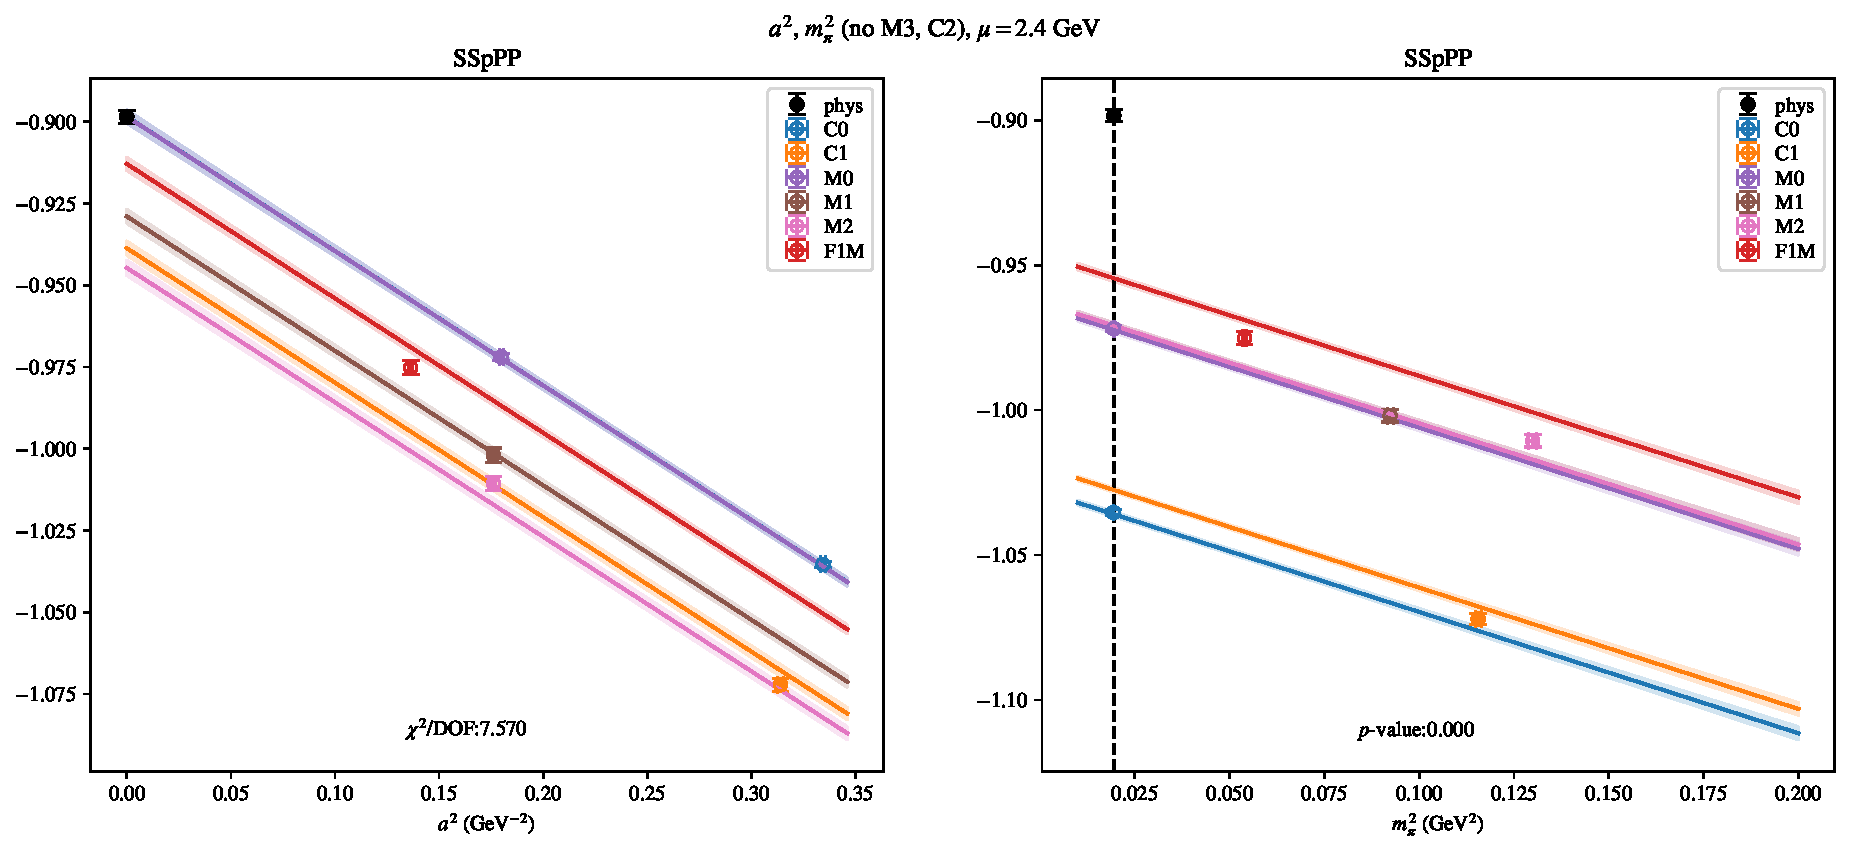
\includepdf[link, pages=-]{VVmAA/SUSY/a2m2mcut_24.pdf}
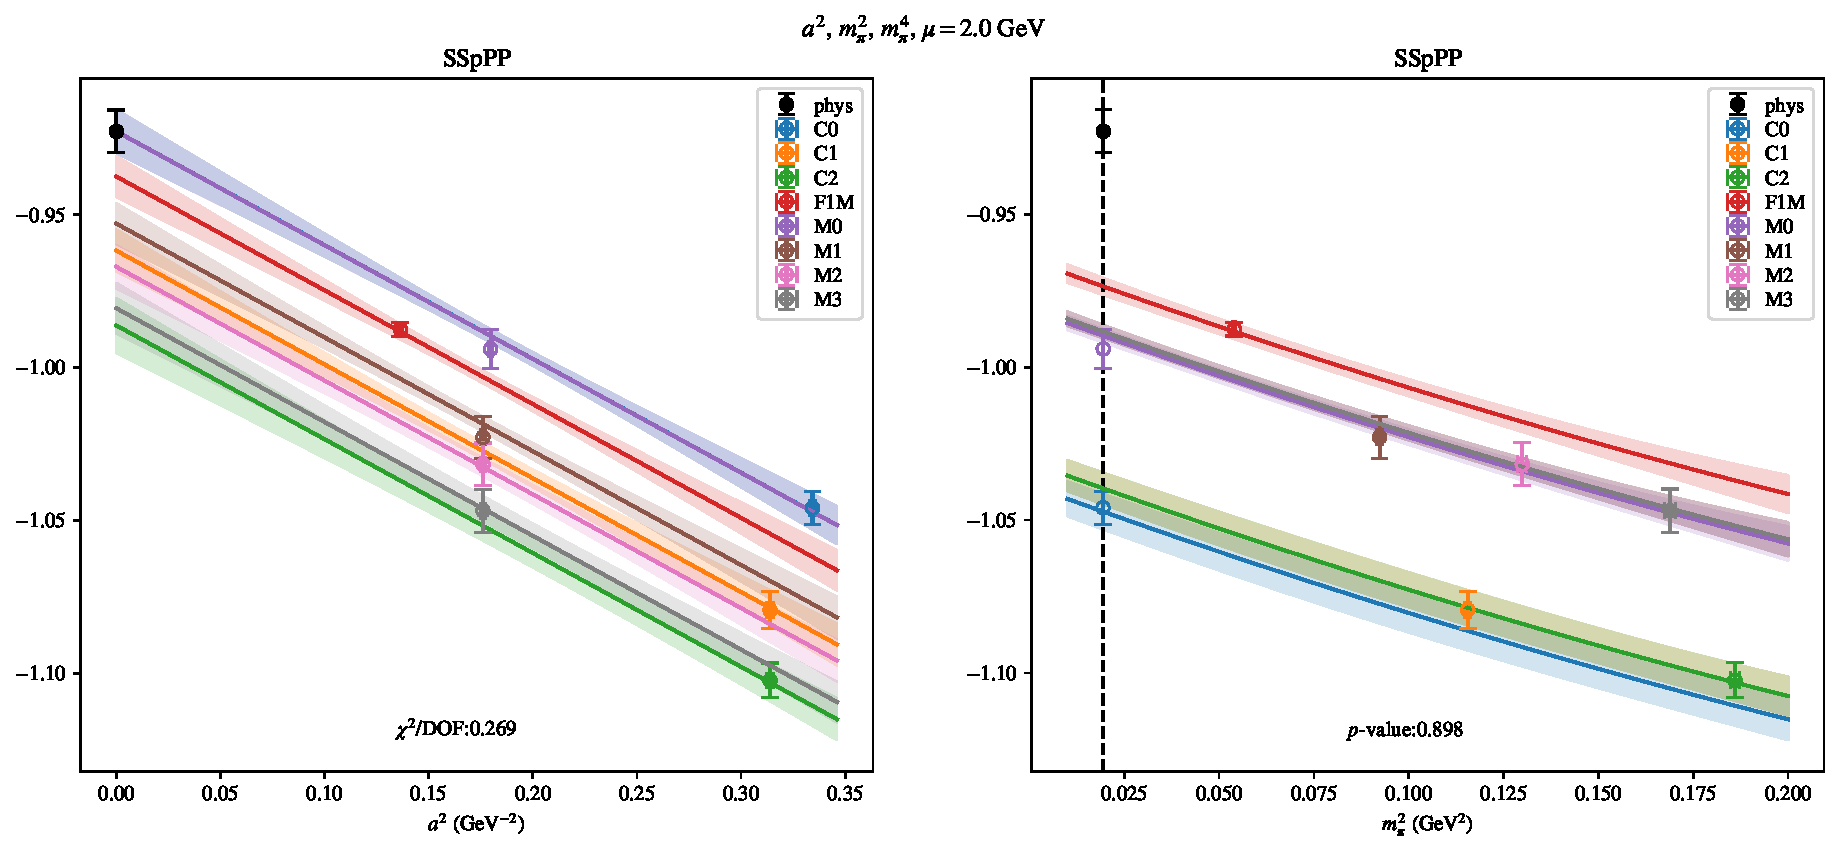
\includepdf[link, pages=-]{VVmAA/SUSY/a2m2m4_20.pdf}
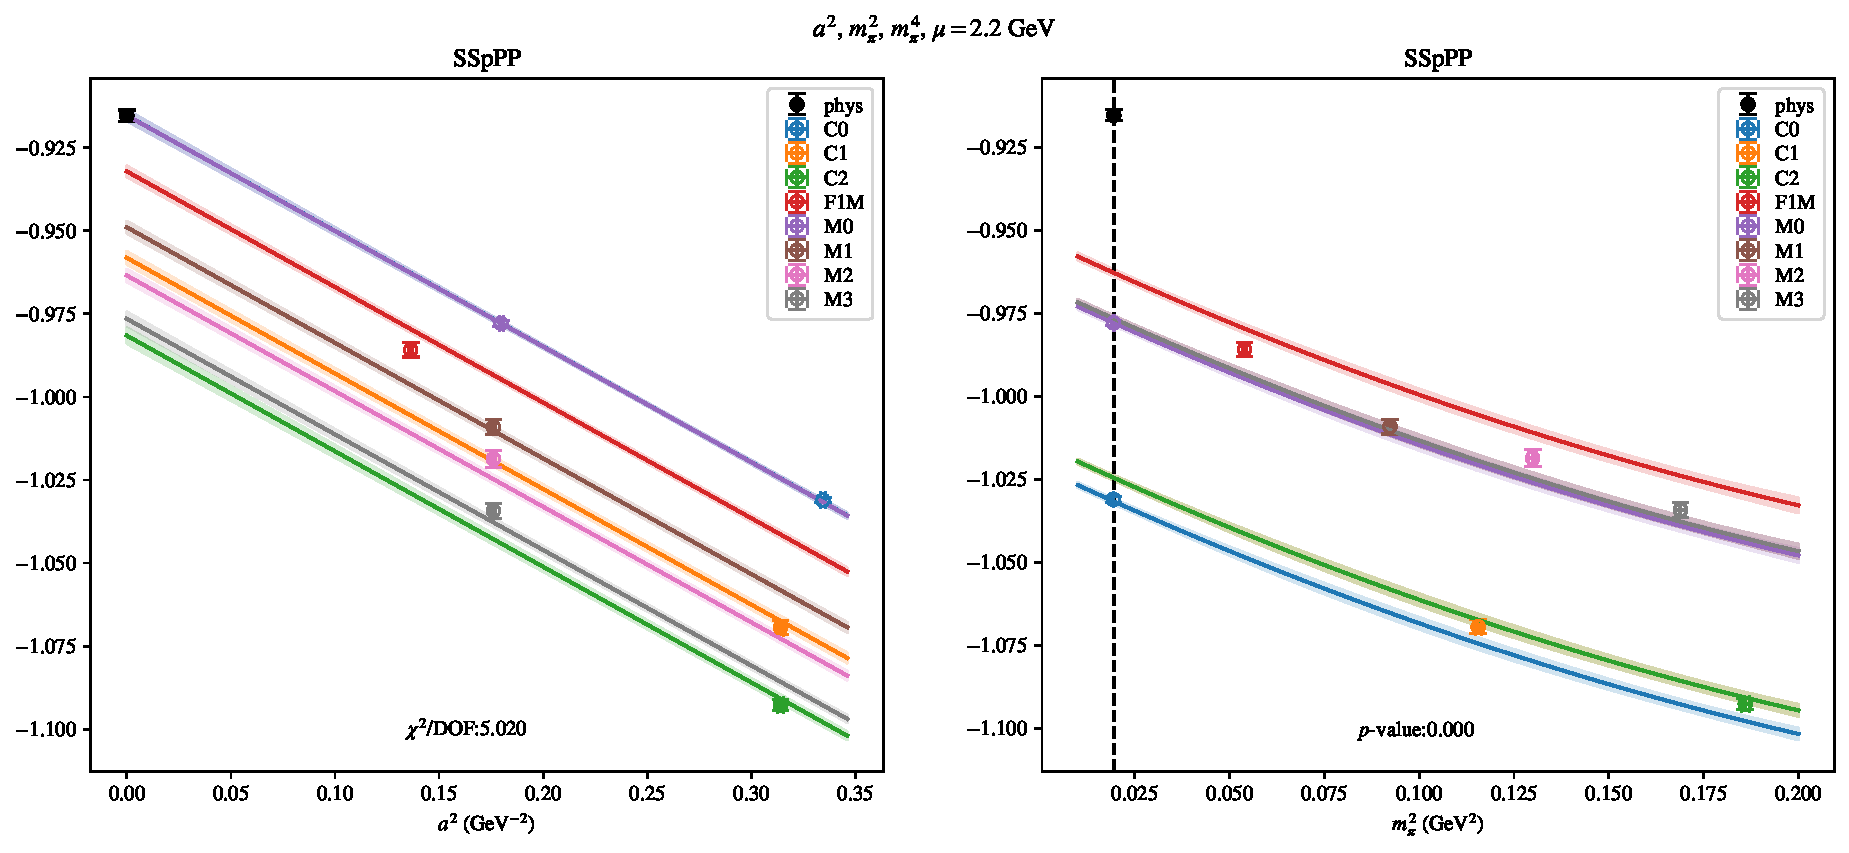
\includepdf[link, pages=-]{VVmAA/SUSY/a2m2m4_22.pdf}
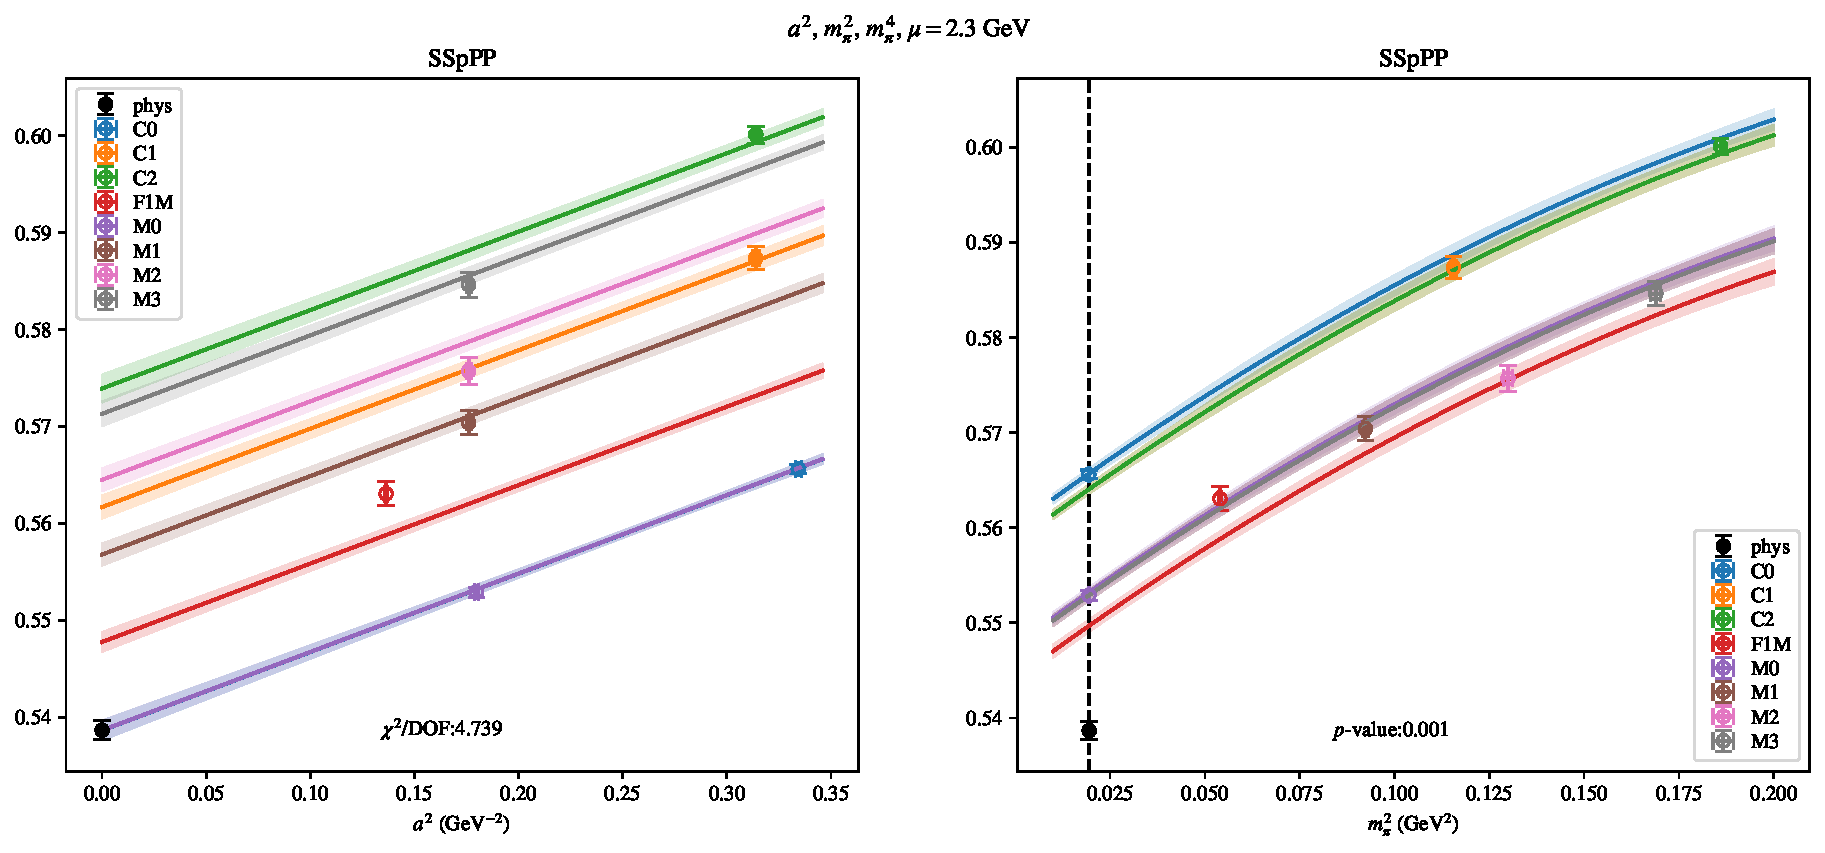
\includepdf[link, pages=-]{VVmAA/SUSY/a2m2m4_23.pdf}
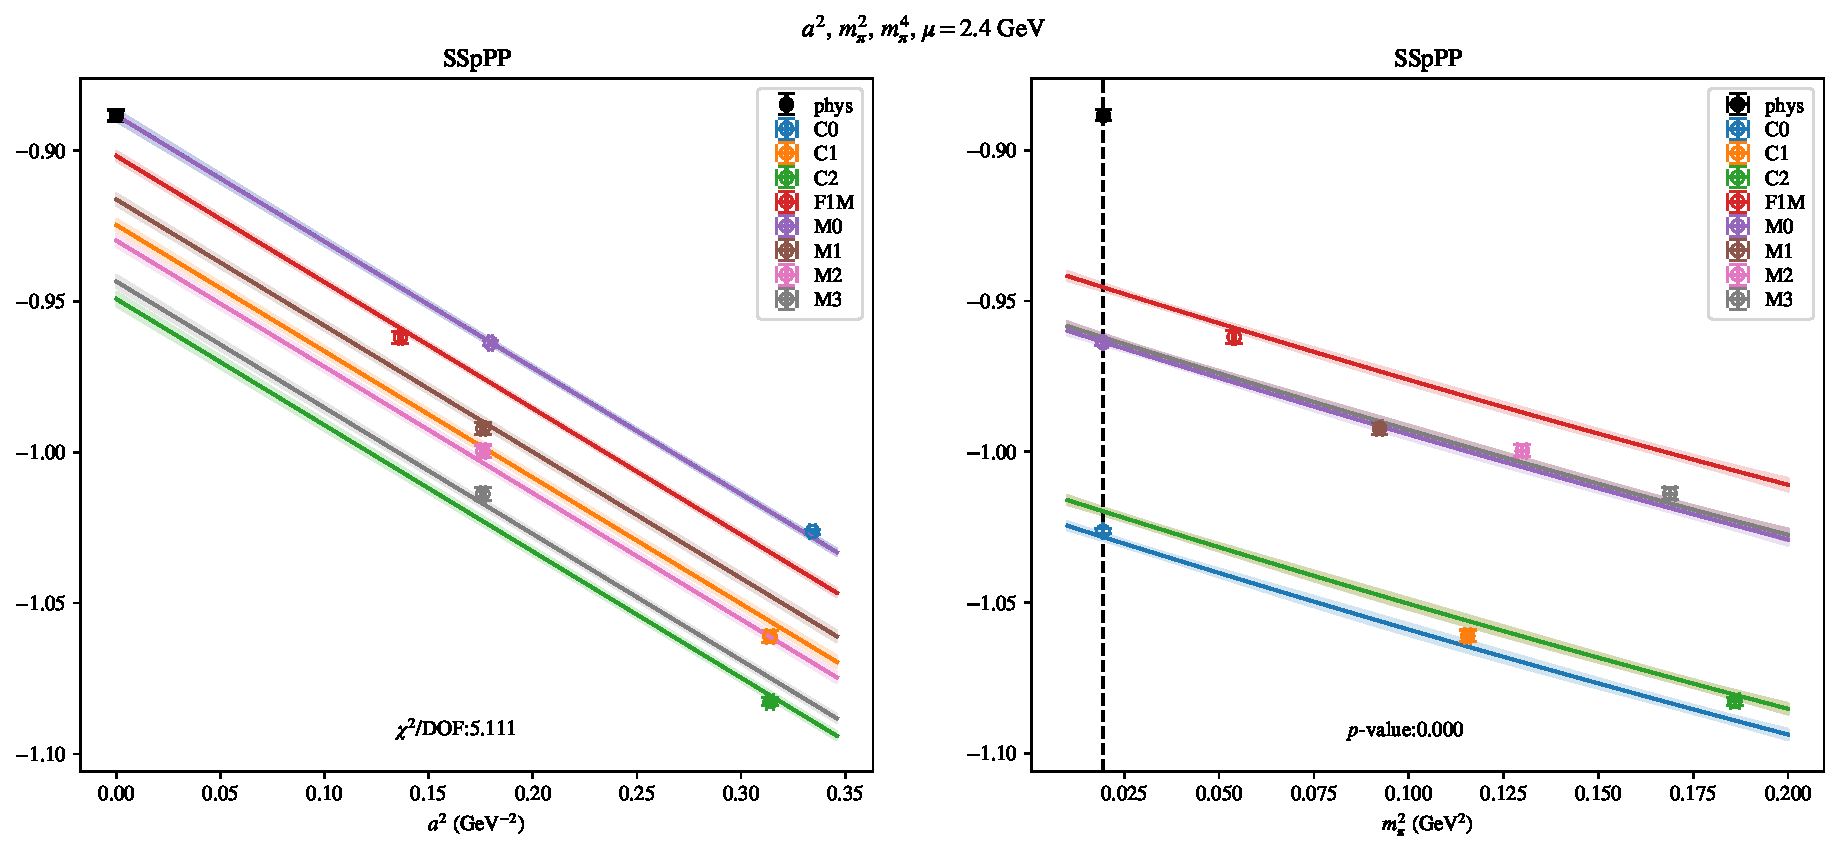
\includepdf[link, pages=-]{VVmAA/SUSY/a2m2m4_24.pdf}
\clearpage
\section{$\mathcal{B}_3$}
\begin{table}[h!]
\begin{center}
\begin{tabular}{|c|c|c|c|c|c|}
\hline
$\mu$ (GeV) & $a^2$, $m_\pi^2$& $a^2$, $m_\pi^2$ (no C)& $a^2$, $a^4$, $m_\pi^2$& $a^2$, $m_\pi^2$ (no M3, C2)& $a^2$, $m_\pi^2$, $m_\pi^4$\\
\hline
2.0& \hyperlink{SSmPP/SUSY/a2m2_20.pdf.1}{\textbf{0.28795(50)}: 9.736 (0.0)} & \hyperlink{SSmPP/SUSY/a2m2noC_20.pdf.1}{\textbf{0.3021(28)}: 4.753 (0.009)} & \hyperlink{SSmPP/SUSY/a2a4m2_20.pdf.1}{\textbf{0.3032(47)}: 9.474 (0.0)} & \hyperlink{SSmPP/SUSY/a2m2mcut_20.pdf.1}{\textbf{0.28777(56)}: 10.884 (0.0)} & \hyperlink{SSmPP/SUSY/a2m2m4_20.pdf.1}{\textbf{0.28687(56)}: 7.09 (0.0)}\\
2.2& \hyperlink{SSmPP/SUSY/a2m2_22.pdf.1}{\textbf{0.27724(48)}: 9.485 (0.0)} & \hyperlink{SSmPP/SUSY/a2m2noC_22.pdf.1}{\textbf{0.2900(27)}: 4.218 (0.015)} & \hyperlink{SSmPP/SUSY/a2a4m2_22.pdf.1}{\textbf{0.2899(45)}: 9.806 (0.0)} & \hyperlink{SSmPP/SUSY/a2m2mcut_22.pdf.1}{\textbf{0.27720(54)}: 10.753 (0.0)} & \hyperlink{SSmPP/SUSY/a2m2m4_22.pdf.1}{\textbf{0.27630(54)}: 7.863 (0.0)}\\
2.3& \hyperlink{SSmPP/SUSY/a2m2_23.pdf.1}{\textbf{0.27251(48)}: 9.315 (0.0)} & \hyperlink{SSmPP/SUSY/a2m2noC_23.pdf.1}{\textbf{0.2855(27)}: 3.921 (0.02)} & \hyperlink{SSmPP/SUSY/a2a4m2_23.pdf.1}{\textbf{0.2857(45)}: 9.361 (0.0)} & \hyperlink{SSmPP/SUSY/a2m2mcut_23.pdf.1}{\textbf{0.27250(54)}: 10.821 (0.0)} & \hyperlink{SSmPP/SUSY/a2m2m4_23.pdf.1}{\textbf{0.27161(54)}: 7.938 (0.0)}\\
2.4& \hyperlink{SSmPP/SUSY/a2m2_24.pdf.1}{\textbf{0.26859(47)}: 9.572 (0.0)} & \hyperlink{SSmPP/SUSY/a2m2noC_24.pdf.1}{\textbf{0.2807(26)}: 3.471 (0.031)} & \hyperlink{SSmPP/SUSY/a2a4m2_24.pdf.1}{\textbf{0.2792(44)}: 10.454 (0.0)} & \hyperlink{SSmPP/SUSY/a2m2mcut_24.pdf.1}{\textbf{0.26872(53)}: 10.987 (0.0)} & \hyperlink{SSmPP/SUSY/a2m2m4_24.pdf.1}{\textbf{0.26781(54)}: 9.099 (0.0)}\\
\hline
\end{tabular}
\caption{Physical point value from chiral and continuum extrapolation at renormalisation scale $\mu$. Entries are \textbf{value(error)}: $\chi^2/\text{DOF}$ ($p$-value).}
\end{center}
\end{table}
\begin{table}[h!]
\begin{center}
\begin{tabular}{|c c|c|c|c|c|c|}
\hline
$\mu$ (GeV) &  & $a^2$, $m_\pi^2$& $a^2$, $m_\pi^2$ (no C)& $a^2$, $a^4$, $m_\pi^2$& $a^2$, $m_\pi^2$ (no M3, C2)& $a^2$, $m_\pi^2$, $m_\pi^4$\\
\hline
\multirow{2}{0.5in}{2.0} & $\alpha$ & 0.6457(77)& 0.349(57)& 0.16(14)& 0.6469(86)& 0.6603(86)\\
 & $\beta$ & 0.00803(15)& 0.00721(22)& 0.00778(16)& 0.00882(27)& 0.01176(79)\\
\hline
\multirow{2}{0.5in}{2.2} & $\alpha$ & 0.7492(80)& 0.466(59)& 0.32(14)& 0.7483(89)& 0.7627(89)\\
 & $\beta$ & 0.00813(15)& 0.00722(23)& 0.00791(16)& 0.00882(27)& 0.01146(80)\\
\hline
\multirow{2}{0.5in}{2.3} & $\alpha$ & 0.8050(82)& 0.511(60)& 0.35(14)& 0.8037(91)& 0.8183(91)\\
 & $\beta$ & 0.00812(15)& 0.00720(23)& 0.00789(17)& 0.00877(27)& 0.01135(81)\\
\hline
\multirow{2}{0.5in}{2.4} & $\alpha$ & 0.8550(83)& 0.575(61)& 0.48(15)& 0.8515(92)& 0.8670(93)\\
 & $\beta$ & 0.00820(16)& 0.00715(23)& 0.00801(17)& 0.00876(27)& 0.01105(81)\\
\hline
\end{tabular}
\caption{Fit values of coefficients in $Q = Q_{phys} + \mathbf{\alpha} a^2 + \mathbf{\beta}\left(\frac{m_\pi^2}{f_\pi^2}-\frac{m_{\pi,PDG}^2}{f_\pi^2}\right) + \ldots$.}
\end{center}
\end{table}
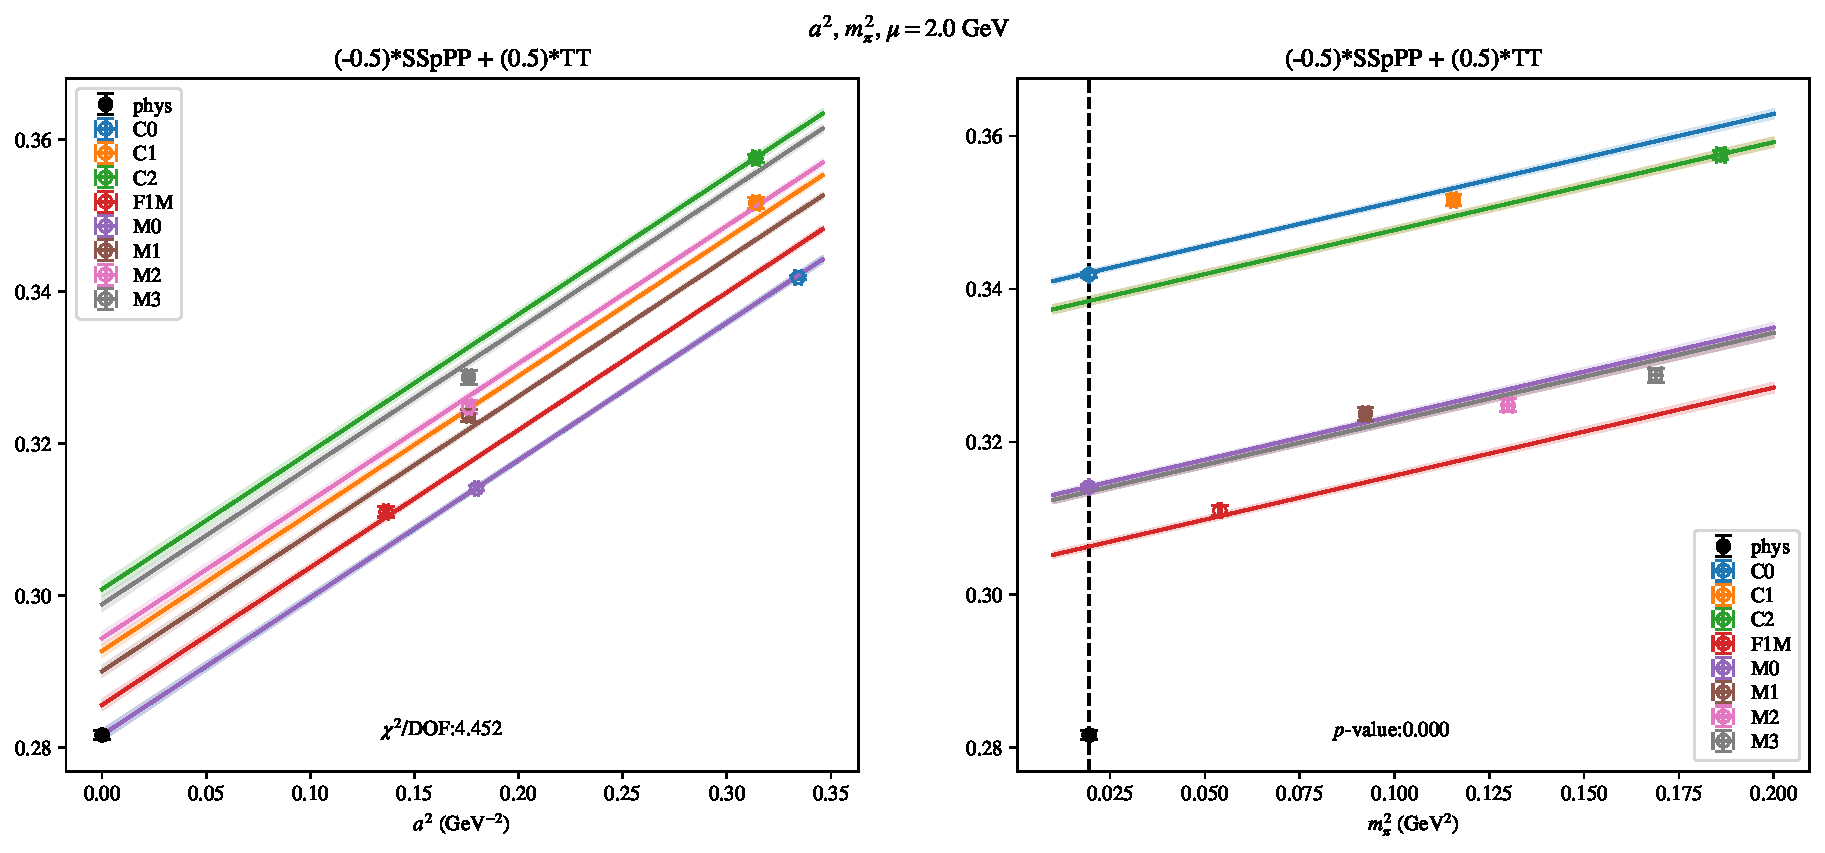
\includepdf[link, pages=-]{SSmPP/SUSY/a2m2_20.pdf}
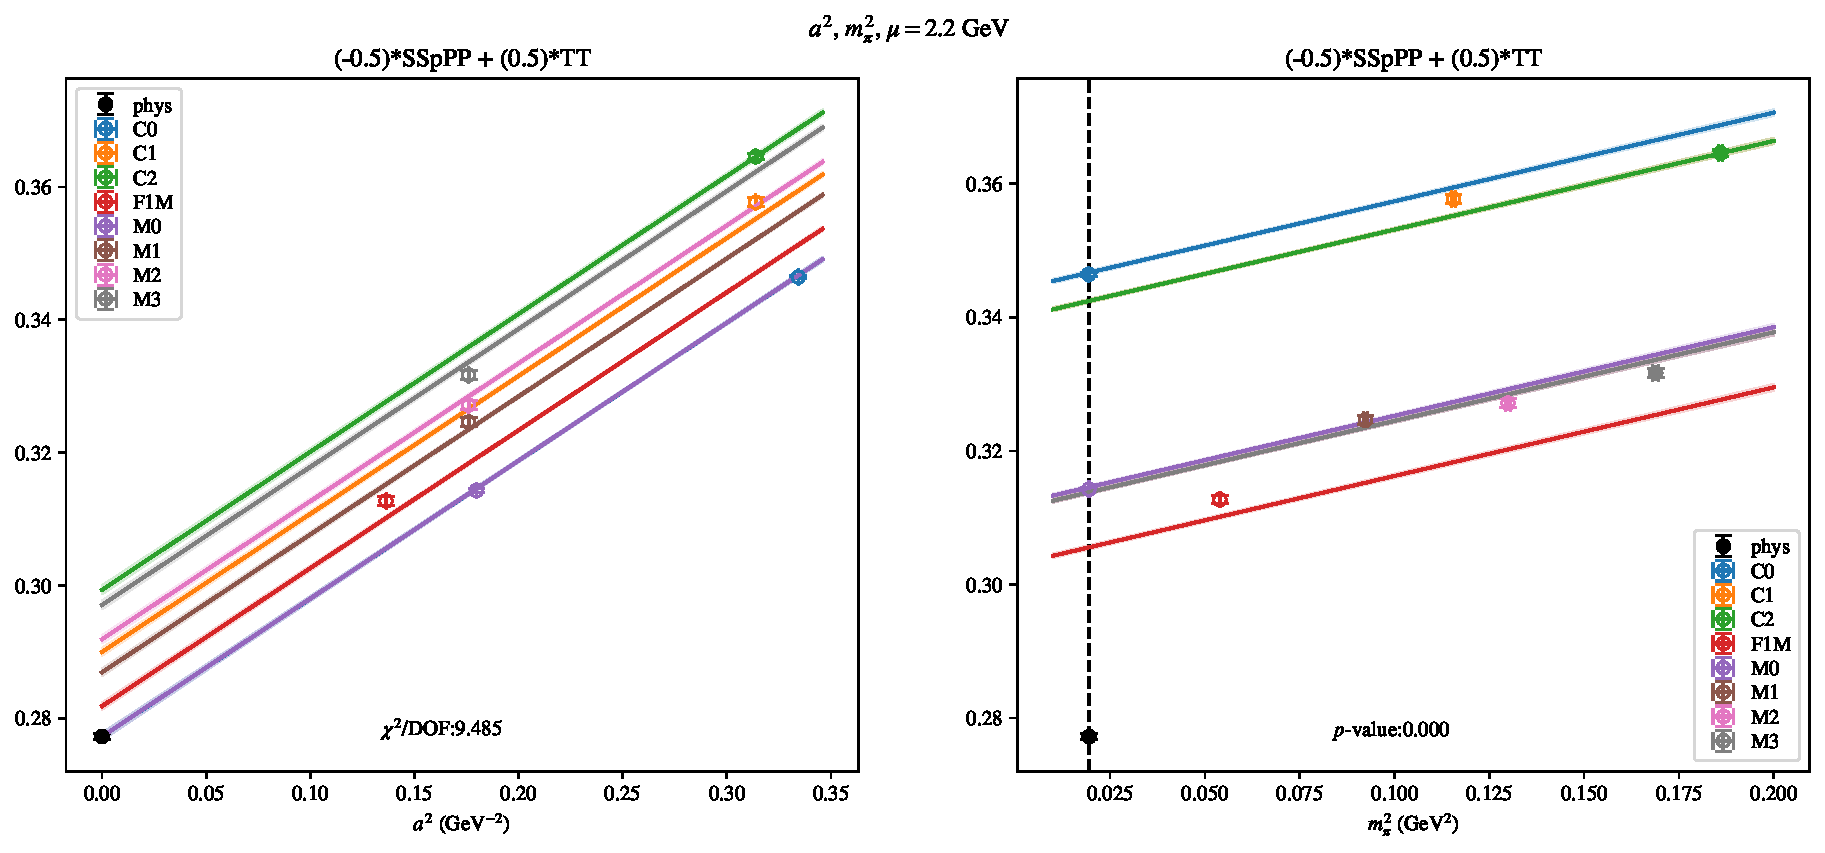
\includepdf[link, pages=-]{SSmPP/SUSY/a2m2_22.pdf}
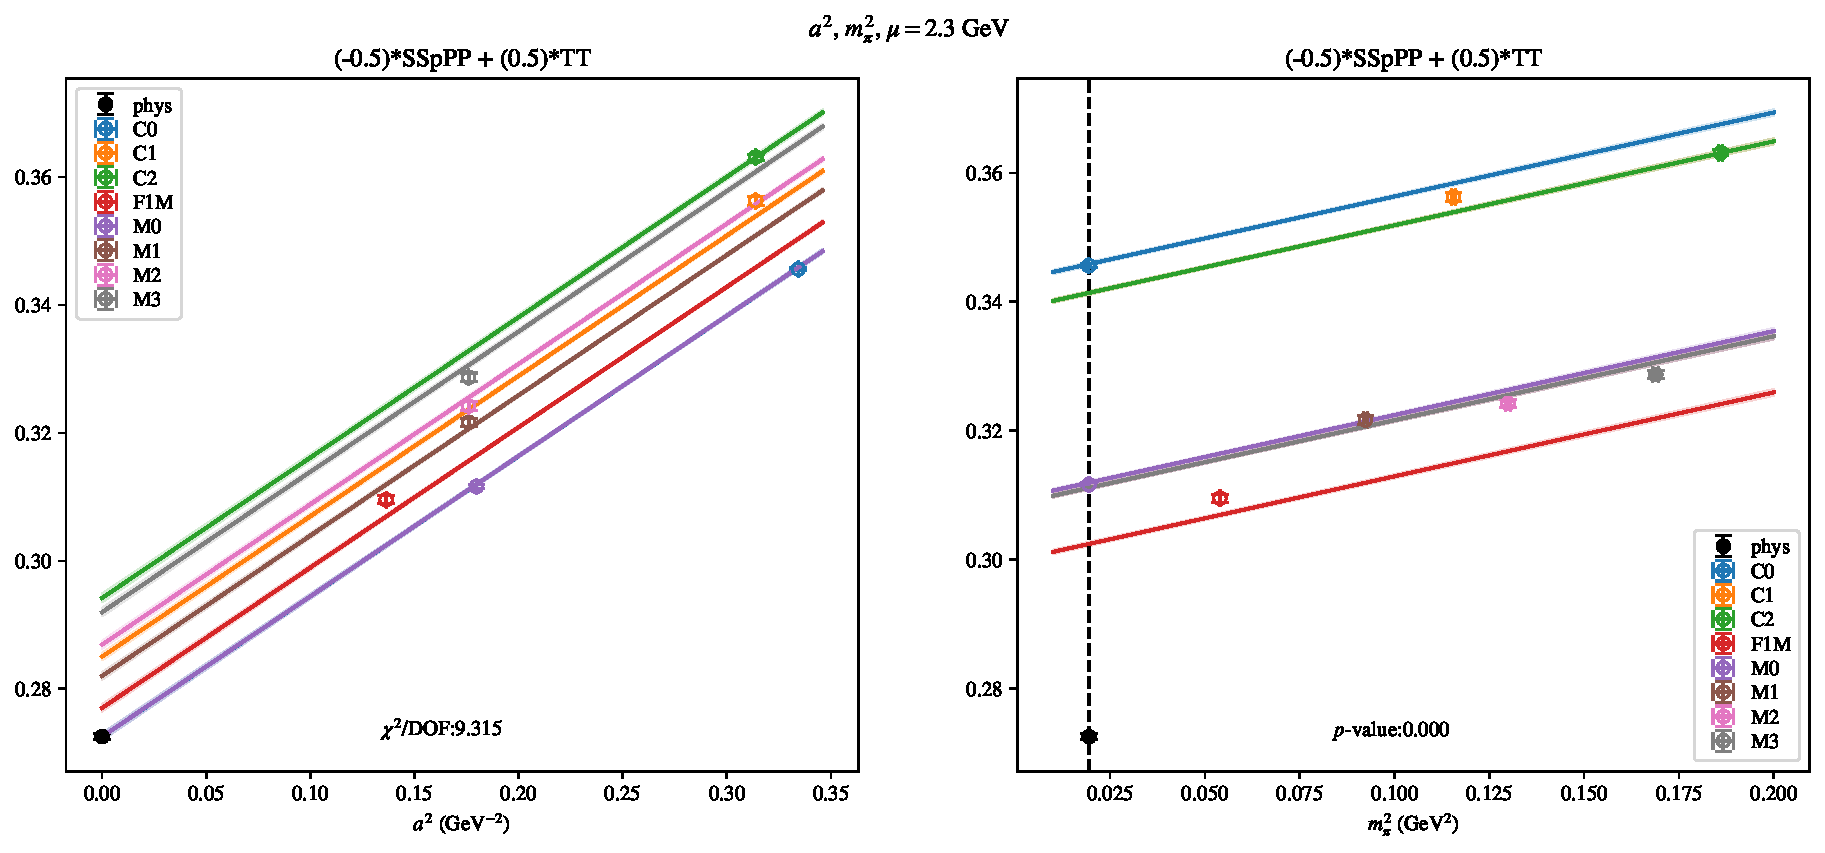
\includepdf[link, pages=-]{SSmPP/SUSY/a2m2_23.pdf}
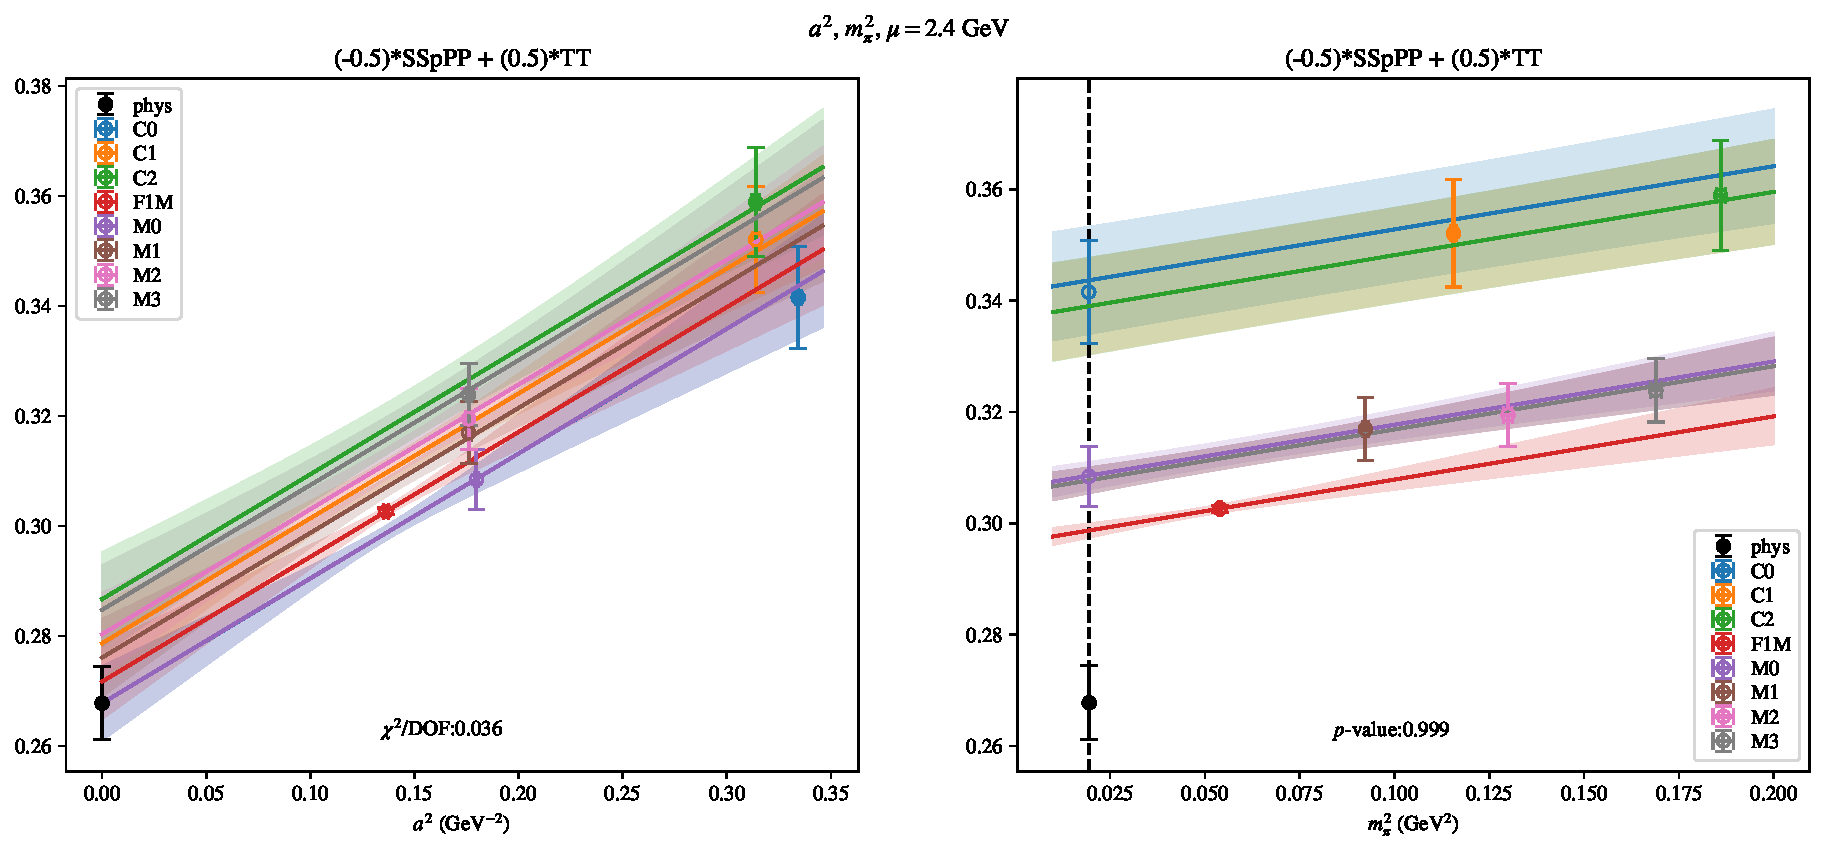
\includepdf[link, pages=-]{SSmPP/SUSY/a2m2_24.pdf}
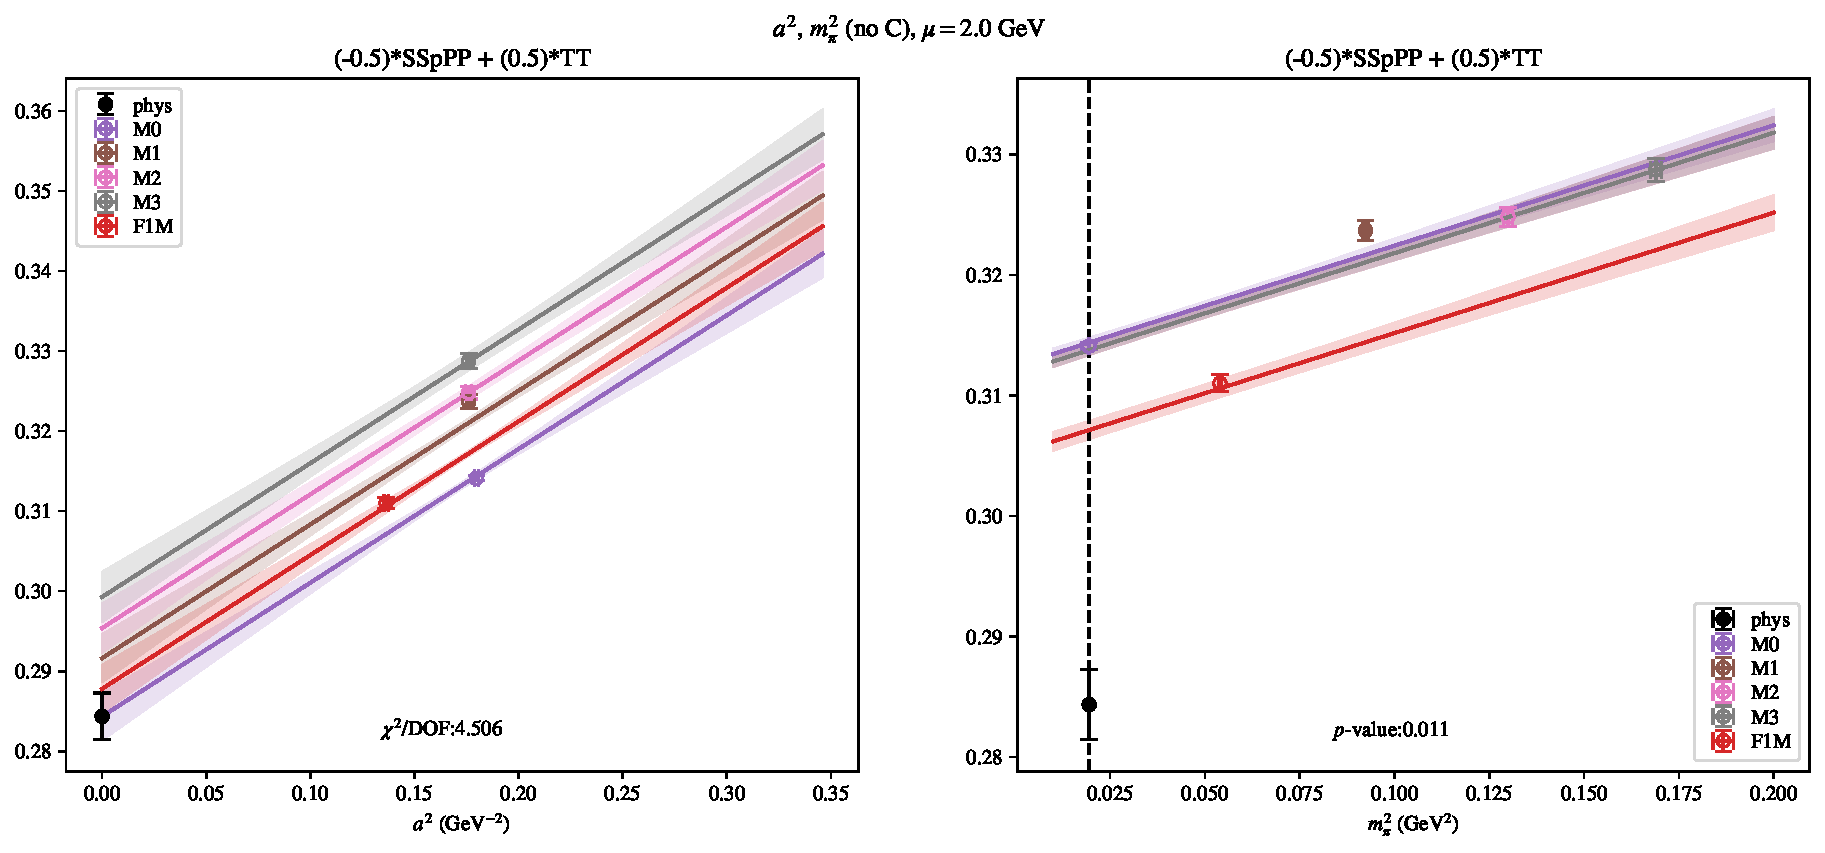
\includepdf[link, pages=-]{SSmPP/SUSY/a2m2noC_20.pdf}
\includepdf[link, pages=-]{SSmPP/SUSY/a2m2noC_22.pdf}
\includepdf[link, pages=-]{SSmPP/SUSY/a2m2noC_23.pdf}
\includepdf[link, pages=-]{SSmPP/SUSY/a2m2noC_24.pdf}
\includepdf[link, pages=-]{SSmPP/SUSY/a2a4m2_20.pdf}
\includepdf[link, pages=-]{SSmPP/SUSY/a2a4m2_22.pdf}
\includepdf[link, pages=-]{SSmPP/SUSY/a2a4m2_23.pdf}
\includepdf[link, pages=-]{SSmPP/SUSY/a2a4m2_24.pdf}
\includepdf[link, pages=-]{SSmPP/SUSY/a2m2mcut_20.pdf}
\includepdf[link, pages=-]{SSmPP/SUSY/a2m2mcut_22.pdf}
\includepdf[link, pages=-]{SSmPP/SUSY/a2m2mcut_23.pdf}
\includepdf[link, pages=-]{SSmPP/SUSY/a2m2mcut_24.pdf}
\includepdf[link, pages=-]{SSmPP/SUSY/a2m2m4_20.pdf}
\includepdf[link, pages=-]{SSmPP/SUSY/a2m2m4_22.pdf}
\includepdf[link, pages=-]{SSmPP/SUSY/a2m2m4_23.pdf}
\includepdf[link, pages=-]{SSmPP/SUSY/a2m2m4_24.pdf}
\clearpage
\section{$\mathcal{B}_4$}
\begin{table}[h!]
\begin{center}
\begin{tabular}{|c|c|c|c|c|c|}
\hline
$\mu$ (GeV) & $a^2$, $m_\pi^2$& $a^2$, $m_\pi^2$ (no C)& $a^2$, $a^4$, $m_\pi^2$& $a^2$, $m_\pi^2$ (no M3, C2)& $a^2$, $m_\pi^2$, $m_\pi^4$\\
\hline
2.0& \hyperlink{SSpPP/SUSY/a2m2_20.pdf.1}{\textbf{1.8415(28)}: 3.883 (0.002)} & \hyperlink{SSpPP/SUSY/a2m2noC_20.pdf.1}{\textbf{1.789(12)}: 1.32 (0.267)} & \hyperlink{SSpPP/SUSY/a2a4m2_20.pdf.1}{\textbf{1.751(20)}: 0.69 (0.598)} & \hyperlink{SSpPP/SUSY/a2m2mcut_20.pdf.1}{\textbf{1.8422(29)}: 6.027 (0.0)} & \hyperlink{SSpPP/SUSY/a2m2m4_20.pdf.1}{\textbf{1.8442(30)}: 3.778 (0.004)}\\
2.2& \hyperlink{SSpPP/SUSY/a2m2_22.pdf.1}{\textbf{1.8330(26)}: 5.107 (0.0)} & \hyperlink{SSpPP/SUSY/a2m2noC_22.pdf.1}{\textbf{1.774(12)}: 1.584 (0.205)} & \hyperlink{SSpPP/SUSY/a2a4m2_22.pdf.1}{\textbf{1.735(20)}: 0.971 (0.422)} & \hyperlink{SSpPP/SUSY/a2m2mcut_22.pdf.1}{\textbf{1.8336(28)}: 7.804 (0.0)} & \hyperlink{SSpPP/SUSY/a2m2m4_22.pdf.1}{\textbf{1.8362(29)}: 4.913 (0.001)}\\
2.3& \hyperlink{SSpPP/SUSY/a2m2_23.pdf.1}{\textbf{1.8299(26)}: 5.463 (0.0)} & \hyperlink{SSpPP/SUSY/a2m2noC_23.pdf.1}{\textbf{1.769(12)}: 1.725 (0.178)} & \hyperlink{SSpPP/SUSY/a2a4m2_23.pdf.1}{\textbf{1.730(20)}: 1.148 (0.332)} & \hyperlink{SSpPP/SUSY/a2m2mcut_23.pdf.1}{\textbf{1.8305(28)}: 8.246 (0.0)} & \hyperlink{SSpPP/SUSY/a2m2m4_23.pdf.1}{\textbf{1.8333(28)}: 5.181 (0.0)}\\
2.4& \hyperlink{SSpPP/SUSY/a2m2_24.pdf.1}{\textbf{1.8276(26)}: 6.108 (0.0)} & \hyperlink{SSpPP/SUSY/a2m2noC_24.pdf.1}{\textbf{1.764(12)}: 1.916 (0.147)} & \hyperlink{SSpPP/SUSY/a2a4m2_24.pdf.1}{\textbf{1.722(20)}: 1.219 (0.3)} & \hyperlink{SSpPP/SUSY/a2m2mcut_24.pdf.1}{\textbf{1.8284(28)}: 9.184 (0.0)} & \hyperlink{SSpPP/SUSY/a2m2m4_24.pdf.1}{\textbf{1.8313(28)}: 5.648 (0.0)}\\
\hline
\end{tabular}
\caption{Physical point value from chiral and continuum extrapolation at renormalisation scale $\mu$. Entries are \textbf{value(error)}: $\chi^2/\text{DOF}$ ($p$-value).}
\end{center}
\end{table}
\begin{table}[h!]
\begin{center}
\begin{tabular}{|c c|c|c|c|c|c|}
\hline
$\mu$ (GeV) &  & $a^2$, $m_\pi^2$& $a^2$, $m_\pi^2$ (no C)& $a^2$, $a^4$, $m_\pi^2$& $a^2$, $m_\pi^2$ (no M3, C2)& $a^2$, $m_\pi^2$, $m_\pi^4$\\
\hline
\multirow{2}{0.5in}{2.0} & $\alpha$ & 0.0712(55)& 0.242(42)& 0.53(11)& 0.0701(59)& 0.0663(59)\\
 & $\beta$ & -0.0001(11)& -0.0002(20)& -0.0003(12)& -0.0003(21)& -0.0014(62)\\
\hline
\multirow{2}{0.5in}{2.2} & $\alpha$ & 0.0723(53)& 0.268(42)& 0.58(11)& 0.0715(58)& 0.0664(58)\\
 & $\beta$ & -0.0002(11)& -0.0003(19)& -0.0004(12)& -0.0004(20)& -0.0017(61)\\
\hline
\multirow{2}{0.5in}{2.3} & $\alpha$ & 0.0735(53)& 0.276(42)& 0.59(11)& 0.0727(58)& 0.0673(58)\\
 & $\beta$ & -0.0003(11)& -0.0003(19)& -0.0005(12)& -0.0005(20)& -0.0019(61)\\
\hline
\multirow{2}{0.5in}{2.4} & $\alpha$ & 0.0744(53)& 0.287(43)& 0.63(11)& 0.0732(58)& 0.0677(58)\\
 & $\beta$ & -0.0003(11)& -0.0004(19)& -0.0005(12)& -0.0006(20)& -0.0021(61)\\
\hline
\end{tabular}
\caption{Fit values of coefficients in $Q = Q_{phys} + \mathbf{\alpha} a^2 + \mathbf{\beta}\left(\frac{m_\pi^2}{f_\pi^2}-\frac{m_{\pi,PDG}^2}{f_\pi^2}\right) + \ldots$.}
\end{center}
\end{table}
\includepdf[link, pages=-]{SSpPP/SUSY/a2m2_20.pdf}
\includepdf[link, pages=-]{SSpPP/SUSY/a2m2_22.pdf}
\includepdf[link, pages=-]{SSpPP/SUSY/a2m2_23.pdf}
\includepdf[link, pages=-]{SSpPP/SUSY/a2m2_24.pdf}
\includepdf[link, pages=-]{SSpPP/SUSY/a2m2noC_20.pdf}
\includepdf[link, pages=-]{SSpPP/SUSY/a2m2noC_22.pdf}
\includepdf[link, pages=-]{SSpPP/SUSY/a2m2noC_23.pdf}
\includepdf[link, pages=-]{SSpPP/SUSY/a2m2noC_24.pdf}
\includepdf[link, pages=-]{SSpPP/SUSY/a2a4m2_20.pdf}
\includepdf[link, pages=-]{SSpPP/SUSY/a2a4m2_22.pdf}
\includepdf[link, pages=-]{SSpPP/SUSY/a2a4m2_23.pdf}
\includepdf[link, pages=-]{SSpPP/SUSY/a2a4m2_24.pdf}
\includepdf[link, pages=-]{SSpPP/SUSY/a2m2mcut_20.pdf}
\includepdf[link, pages=-]{SSpPP/SUSY/a2m2mcut_22.pdf}
\includepdf[link, pages=-]{SSpPP/SUSY/a2m2mcut_23.pdf}
\includepdf[link, pages=-]{SSpPP/SUSY/a2m2mcut_24.pdf}
\includepdf[link, pages=-]{SSpPP/SUSY/a2m2m4_20.pdf}
\includepdf[link, pages=-]{SSpPP/SUSY/a2m2m4_22.pdf}
\includepdf[link, pages=-]{SSpPP/SUSY/a2m2m4_23.pdf}
\includepdf[link, pages=-]{SSpPP/SUSY/a2m2m4_24.pdf}
\clearpage
\section{$\mathcal{B}_5$}
\begin{table}[h!]
\begin{center}
\begin{tabular}{|c|c|c|c|c|c|}
\hline
$\mu$ (GeV) & $a^2$, $m_\pi^2$& $a^2$, $m_\pi^2$ (no C)& $a^2$, $a^4$, $m_\pi^2$& $a^2$, $m_\pi^2$ (no M3, C2)& $a^2$, $m_\pi^2$, $m_\pi^4$\\
\hline
2.0& \hyperlink{TT/SUSY/a2m2_20.pdf.1}{\textbf{0.50643(75)}: 3.824 (0.002)} & \hyperlink{TT/SUSY/a2m2noC_20.pdf.1}{\textbf{0.4925(44)}: 3.308 (0.037)} & \hyperlink{TT/SUSY/a2a4m2_20.pdf.1}{\textbf{0.4817(68)}: 1.778 (0.13)} & \hyperlink{TT/SUSY/a2m2mcut_20.pdf.1}{\textbf{0.50679(77)}: 4.93 (0.002)} & \hyperlink{TT/SUSY/a2m2m4_20.pdf.1}{\textbf{0.50722(77)}: 2.881 (0.021)}\\
2.2& \hyperlink{TT/SUSY/a2m2_22.pdf.1}{\textbf{0.50981(70)}: 4.471 (0.0)} & \hyperlink{TT/SUSY/a2m2noC_22.pdf.1}{\textbf{0.4941(43)}: 3.669 (0.026)} & \hyperlink{TT/SUSY/a2a4m2_22.pdf.1}{\textbf{0.4845(65)}: 2.104 (0.077)} & \hyperlink{TT/SUSY/a2m2mcut_22.pdf.1}{\textbf{0.51014(74)}: 5.603 (0.001)} & \hyperlink{TT/SUSY/a2m2m4_22.pdf.1}{\textbf{0.51070(73)}: 3.281 (0.011)}\\
2.3& \hyperlink{TT/SUSY/a2m2_23.pdf.1}{\textbf{0.51153(69)}: 4.842 (0.0)} & \hyperlink{TT/SUSY/a2m2noC_23.pdf.1}{\textbf{0.4948(43)}: 3.67 (0.025)} & \hyperlink{TT/SUSY/a2a4m2_23.pdf.1}{\textbf{0.4853(64)}: 2.223 (0.064)} & \hyperlink{TT/SUSY/a2m2mcut_23.pdf.1}{\textbf{0.51184(73)}: 6.094 (0.0)} & \hyperlink{TT/SUSY/a2m2m4_23.pdf.1}{\textbf{0.51244(72)}: 3.607 (0.006)}\\
2.4& \hyperlink{TT/SUSY/a2m2_24.pdf.1}{\textbf{0.51299(69)}: 5.105 (0.0)} & \hyperlink{TT/SUSY/a2m2noC_24.pdf.1}{\textbf{0.4958(42)}: 3.783 (0.023)} & \hyperlink{TT/SUSY/a2a4m2_24.pdf.1}{\textbf{0.4865(64)}: 2.397 (0.048)} & \hyperlink{TT/SUSY/a2m2mcut_24.pdf.1}{\textbf{0.51330(72)}: 6.353 (0.0)} & \hyperlink{TT/SUSY/a2m2m4_24.pdf.1}{\textbf{0.51392(72)}: 3.755 (0.005)}\\
\hline
\end{tabular}
\caption{Physical point value from chiral and continuum extrapolation at renormalisation scale $\mu$. Entries are \textbf{value(error)}: $\chi^2/\text{DOF}$ ($p$-value).}
\end{center}
\end{table}
\begin{table}[h!]
\begin{center}
\begin{tabular}{|c c|c|c|c|c|c|}
\hline
$\mu$ (GeV) &  & $a^2$, $m_\pi^2$& $a^2$, $m_\pi^2$ (no C)& $a^2$, $a^4$, $m_\pi^2$& $a^2$, $m_\pi^2$ (no M3, C2)& $a^2$, $m_\pi^2$, $m_\pi^4$\\
\hline
\multirow{2}{0.5in}{2.0} & $\alpha$ & -0.177(50)& -0.01(51)& 0.26(12)& -0.179(51)& -0.182(51)\\
 & $\beta$ & 0.00193(11)& 0.00179(20)& 0.00186(12)& 0.00156(21)& 0.00021(64)\\
\hline
\multirow{2}{0.5in}{2.2} & $\alpha$ & -0.222(47)& -0.04(49)& 0.22(12)& -0.224(49)& -0.228(49)\\
 & $\beta$ & 0.00165(11)& 0.00160(19)& 0.00156(12)& 0.00127(20)& -0.0001(62)\\
\hline
\multirow{2}{0.5in}{2.3} & $\alpha$ & -0.245(46)& -0.05(48)& 0.21(12)& -0.247(48)& -0.251(48)\\
 & $\beta$ & 0.00155(11)& 0.00152(19)& 0.00145(12)& 0.00116(20)& -0.0003(61)\\
\hline
\multirow{2}{0.5in}{2.4} & $\alpha$ & -0.266(45)& -0.07(48)& 0.20(12)& -0.268(47)& -0.272(47)\\
 & $\beta$ & 0.00144(11)& 0.00143(19)& 0.00134(11)& 0.00104(20)& -0.0004(61)\\
\hline
\end{tabular}
\caption{Fit values of coefficients in $Q = Q_{phys} + \mathbf{\alpha} a^2 + \mathbf{\beta}\left(\frac{m_\pi^2}{f_\pi^2}-\frac{m_{\pi,PDG}^2}{f_\pi^2}\right) + \ldots$.}
\end{center}
\end{table}
\includepdf[link, pages=-]{TT/SUSY/a2m2_20.pdf}
\includepdf[link, pages=-]{TT/SUSY/a2m2_22.pdf}
\includepdf[link, pages=-]{TT/SUSY/a2m2_23.pdf}
\includepdf[link, pages=-]{TT/SUSY/a2m2_24.pdf}
\includepdf[link, pages=-]{TT/SUSY/a2m2noC_20.pdf}
\includepdf[link, pages=-]{TT/SUSY/a2m2noC_22.pdf}
\includepdf[link, pages=-]{TT/SUSY/a2m2noC_23.pdf}
\includepdf[link, pages=-]{TT/SUSY/a2m2noC_24.pdf}
\includepdf[link, pages=-]{TT/SUSY/a2a4m2_20.pdf}
\includepdf[link, pages=-]{TT/SUSY/a2a4m2_22.pdf}
\includepdf[link, pages=-]{TT/SUSY/a2a4m2_23.pdf}
\includepdf[link, pages=-]{TT/SUSY/a2a4m2_24.pdf}
\includepdf[link, pages=-]{TT/SUSY/a2m2mcut_20.pdf}
\includepdf[link, pages=-]{TT/SUSY/a2m2mcut_22.pdf}
\includepdf[link, pages=-]{TT/SUSY/a2m2mcut_23.pdf}
\includepdf[link, pages=-]{TT/SUSY/a2m2mcut_24.pdf}
\includepdf[link, pages=-]{TT/SUSY/a2m2m4_20.pdf}
\includepdf[link, pages=-]{TT/SUSY/a2m2m4_22.pdf}
\includepdf[link, pages=-]{TT/SUSY/a2m2m4_23.pdf}
\includepdf[link, pages=-]{TT/SUSY/a2m2m4_24.pdf}
\clearpage
\end{document}